%----------
%   IMPORTANTE
%----------

% Si nunca has utilizado LaTeX es conveniente que aprendas una serie de conceptos básicos antes de utilizar esta plantilla. Te aconsejamos que leas previamente algún tutorial (puedes encontar muchos en Internet).

% Esta plantilla está basada en las recomendaciones de la guía "Trabajo fin de Máster: Escribir el TFM", que encontrarás en http://uc3m.libguides.com/TFM/escribir
% contiene recomendaciones de la Biblioteca basadas principalmente en estilos APA e IEEE, pero debes seguir siempre las orientaciones de tu Tutor de TFM y la normativa de TFM para tu titulación.

% Encontrarás un ejemplo de TFM realizado con esta misma plantilla en la carpeta "_ejemplo_TFM_2019". Consúltalo porque contiene ejemplos útiles para incorporar tablas, figuras, listados de código, bibliografía, etc.


%----------
%	CONFIGURACIÓN DEL DOCUMENTO
%----------

% Definimos las características del documento y añadimos una serie de paquetes (\usepackage{package}) que agregan funcionalidades a LaTeX.

\documentclass[12pt]{report} %fuente a 12pt

% MÁRGENES: 2,5 cm sup. e inf.; 3 cm izdo. y dcho.
\usepackage[
a4paper,
vmargin=2.5cm,
hmargin=2.7cm
]{geometry}

% INTERLINEADO: Estrecho (6 ptos./interlineado 1,15) o Moderado (6 ptos./interlineado 1,5)
\renewcommand{\baselinestretch}{1.15}
\parskip=6pt

% DEFINICIÓN DE COLORES para portada y listados de código
\usepackage[table]{xcolor}
\definecolor{azulUC3M}{RGB}{0,0,102}
\definecolor{gray97}{gray}{.97}
\definecolor{gray75}{gray}{.75}
\definecolor{gray45}{gray}{.45}

\usepackage{subcaption}

% Soporte para GENERAR PDF/A --es importante de cara a su inclusión en e-Archivo porque es el formato óptimo de preservación y a la generación de metadatos, tal y como se describe en http://uc3m.libguides.com/ld.php?content_id=31389625. En la carpeta incluímos el archivo plantilla_tfg_2017.xmpdata en el que puedes incluir los metadatos que se incorporarán al archivo PDF cuando lo compiles. Ese archivo debe llamarse igual que tu archivo .tex. Puedes ver un ejemplo en esta misma carpeta.
\usepackage[a-1b]{pdfx}

% ENLACES
\usepackage{hyperref}
\hypersetup{colorlinks=true,
	linkcolor=black, % enlaces a partes del documento (p.e. índice) en color negro
	urlcolor=blue} % enlaces a recursos fuera del documento en azul

% EXPRESIONES MATEMATICAS
\usepackage{amsmath,amssymb,amsfonts,amsthm}

\usepackage{txfonts} 
\usepackage[T1]{fontenc}
\usepackage[utf8]{inputenc}

\usepackage[english]{babel} 
\usepackage[babel, english=american]{csquotes}
\AtBeginEnvironment{quote}{\small}

% diseño de PIE DE PÁGINA
\usepackage{fancyhdr}
\pagestyle{fancy}
\fancyhf{}
\renewcommand{\headrulewidth}{0pt}
\rfoot{\thepage}
\fancypagestyle{plain}{\pagestyle{fancy}}

% DISEÑO DE LOS TÍTULOS de las partes del trabajo (capítulos y epígrafes o subcapítulos)
\usepackage{titlesec}
\usepackage{titletoc}
\titleformat{\chapter}[block]
{\large\bfseries\filcenter}
{\thechapter.}
{5pt}
{\MakeUppercase}
{}
\titlespacing{\chapter}{0pt}{0pt}{*3}
\titlecontents{chapter}
[0pt]                                               
{}
{\contentsmargin{0pt}\thecontentslabel.\enspace\uppercase}
{\contentsmargin{0pt}\uppercase}                        
{\titlerule*[.7pc]{.}\contentspage}                 

\titleformat{\section}
{\bfseries}
{\thesection.}
{5pt}
{}
\titlecontents{section}
[5pt]                                               
{}
{\contentsmargin{0pt}\thecontentslabel.\enspace}
{\contentsmargin{0pt}}
{\titlerule*[.7pc]{.}\contentspage}

\titleformat{\subsection}
{\normalsize\bfseries}
{\thesubsection.}
{5pt}
{}
\titlecontents{subsection}
[10pt]                                               
{}
{\contentsmargin{0pt}                          
	\thecontentslabel.\enspace}
{\contentsmargin{0pt}}                        
{\titlerule*[.7pc]{.}\contentspage}  


% DISEÑO DE TABLAS. Puedes elegir entre el estilo para ingeniería o para ciencias sociales y humanidades. Por defecto, está activado el estilo de ingeniería. Si deseas utilizar el otro, comenta las líneas del diseño de ingeniería y descomenta las del diseño de ciencias sociales y humanidades
\usepackage{multirow} %permite combinar celdas 
\usepackage{caption} %para personalizar el título de tablas y figuras
\usepackage{floatrow} %utilizamos este paquete y sus macros \ttabbox y \ffigbox para alinear los nombres de tablas y figuras de acuerdo con el estilo definido. Para su uso ver archivo de ejemplo 
\usepackage{array} % con este paquete podemos definir en la siguiente línea un nuevo tipo de columna para tablas: ancho personalizado y contenido centrado
\newcolumntype{P}[1]{>{\centering\arraybackslash}p{#1}}
\DeclareCaptionFormat{upper}{#1#2\uppercase{#3}\par}
\usepackage{booktabs}

% Diseño de tabla para ingeniería
\captionsetup[table]{
	format=upper,
	justification=centering,
	labelsep=period,
	width=.75\linewidth,
	labelfont=small,
	font=small,
}

%Diseño de tabla para ciencias sociales y humanidades
%\captionsetup[table]{
%	justification=raggedright,
%	labelsep=period,
%	labelfont=small,
%	singlelinecheck=false,
%	font={small,bf}
%}


% DISEÑO DE FIGURAS. Puedes elegir entre el estilo para ingeniería o para ciencias sociales y humanidades. Por defecto, está activado el estilo de ingeniería. Si deseas utilizar el otro, comenta las líneas del diseño de ingeniería y descomenta las del diseño de ciencias sociales y humanidades
\usepackage{graphicx}
\graphicspath{{images/}} %ruta a la carpeta de imágenes

% Diseño de figuras para ingeniería
\captionsetup[figure]{
	format=hang,
	name=Fig.,
	justification=centering,
	singlelinecheck=off,
	labelsep=colon,
	labelfont=small,
	font=small		
}

% Diseño de figuras para ciencias sociales y humanidades
%\captionsetup[figure]{
%	format=hang,
%	name=Figure,
%	singlelinecheck=off,
%	labelsep=period,
%	labelfont=small,
%	font=small		
%}


% NOTAS A PIE DE PÁGINA
\usepackage{chngcntr} %para numeración contínua de las notas al pie
\counterwithout{footnote}{chapter}

% LISTADOS DE CÓDIGO
% soporte y estilo para listados de código. Más información en https://es.wikibooks.org/wiki/Manual_de_LaTeX/Listados_de_código/Listados_con_listings
\usepackage{listings}

% definimos un estilo de listings
\lstdefinestyle{estilo}{ frame=Ltb,
	framerule=0pt,
	aboveskip=0.5cm,
	framextopmargin=3pt,
	framexbottommargin=3pt,
	framexleftmargin=0.4cm,
	framesep=0pt,
	rulesep=.4pt,
	backgroundcolor=\color{gray97},
	rulesepcolor=\color{black},
	%
	basicstyle=\ttfamily\footnotesize,
	keywordstyle=\bfseries,
	stringstyle=\ttfamily,
	showstringspaces = false,
	commentstyle=\color{gray45},     
	%
	numbers=left,
	numbersep=15pt,
	numberstyle=\tiny,
	numberfirstline = false,
	breaklines=true,
	xleftmargin=\parindent
}

\captionsetup[lstlisting]{font=small, labelsep=period}
% fijamos el estilo a utilizar 
\lstset{style=estilo}
\renewcommand{\lstlistingname}{\uppercase{Código}}


%BIBLIOGRAFÍA - PUEDES ELEGIR ENTRE ESTILO IEEE O APA. POR DEFECTO ESTÁ CONFIGURADO IEEE. SI DESEAS USAR APA, COMENTA LAS LÍNEA DE IEEE Y DESCOMENTA LAS DE APA. Si haces cambios en la configuración de la bibliografía y no obtienes los resultados esperados, es recomendable limpiar los archivos auxiliares y volver a compilar en este orden: COMPILAR-BIBLIOGRAFIA-COMPILAR
% Tienes más información sobre cómo generar bibliografía en http://tex.stackexchange.com/questions/154751/biblatex-with-biber-configuring-my-editor-to-avoid-undefined-citations , https://es.sharelatex.com/learn/Bibliography_management_in_LaTeX y en http://www.ctan.org/tex-archive/macros/latex/exptl/biblatex-contrib
% También te recomendamos consultar la guía temática de la Biblioteca sobre citas bibliográficas: http://uc3m.libguides.com/guias_tematicas/citas_bibliograficas/inicio

% CONFIGURACIÓN PARA LA BIBLIOGRAFÍA IEEE
\usepackage[backend=biber, style=ieee, isbn=false,sortcites, maxbibnames=5, minbibnames=1]{biblatex} % Configuración para el estilo de citas de IEEE, recomendado para el área de ingeniería. "maxbibnames" indica que a partir de 5 autores trunque la lista el primero (minbibnames) y añada "et al." tal y como se utiliza en el estilo IEEE.

%CONFIGURACIÓN PARA LA BIBLIOGRAFÍA APA
%\usepackage[style=apa, backend=biber, natbib=true, hyperref=true, uniquelist=false, sortcites]{biblatex}
%\DeclareLanguageMapping{spanish}{spanish-apa}

\addbibresource{citations/websites.bib} % llama al archivo bibliografia.bib que utilizamos de ejemplo


%-------------
%	DOCUMENTO
%-------------

\begin{document}
\pagenumbering{roman} % Se utilizan cifras romanas en la numeración de las páginas previas al cuerpo del trabajo
	
%----------
%	PORTADA
%----------	
\begin{titlepage}
	\begin{sffamily}
	\color{azulUC3M}
	\begin{center}
		\begin{figure}[H] %incluimos el logotipo de la Universidad
			\makebox[\textwidth][c]{
\includegraphics[width=16cm]{Portada_Logo.png}}
		\end{figure}
		\vspace{1cm}
		\begin{Large}
			Master in Big Data Analytics\\			
			Academic Year 2022-2023\\
			\vspace{1cm}		
			\textsl{Master Thesis}
			\bigskip
			
		\end{Large}
		 	{\Huge ``Time-series models to explain the evolution of the electricity prices in the short and the long term''}\\
		 	\vspace*{0.5cm}
	 		\rule{10.5cm}{0.1mm}\\
			\vspace*{0.9cm}
			{\LARGE Pedro Bedmar López}\\
			\vspace*{1cm}
		\begin{Large}
			Supervisor: Francisco Javier Nogales Martín\\
			Madrid, the 10th of September 2023\\
		\end{Large}
	\end{center}
	
	\vfill
	\color{black}
	\begin{footnotesize}
	\noindent\fbox{
	\begin{minipage}{\textwidth}
		\textbf{AVOID PLAGIARISM}\\
		The University uses the \textbf{Turnitin Feedback Studio} program within the Aula Global for the delivery of student work. This program compares the originality of the work delivered by each student with millions of electronic resources and detects those parts of the text that are copied and pasted. Plagiarizing in a TFM is considered a \textbf{Serious Misconduct}, and may result in permanent expulsion from the University.
	\end{minipage}	
	}
	\vspace*{.5cm}\\	
	\noindent
\includegraphics[width=4.2cm]{images/creativecommons.png}\\
	\emph{[Include this code in case you want your Master Thesis published in Open Access University Repository]}\\
	This work is licensed under Creative Commons \textbf{Attribution – Non Commercial – Non Derivatives}

	\end{footnotesize}
	\end{sffamily}
\end{titlepage}

\newpage %página en blanco o de cortesía
\thispagestyle{empty}
\mbox{}

%----------
%	RESUMEN Y PALABRAS CLAVE
%----------	
\renewcommand\abstractname{\large\uppercase{Summary}}
\begin{abstract}
\thispagestyle{plain}
\setcounter{page}{3}
	
	The goal of this Master Thesis is to develop time-series models to capture the main factors affecting electricity prices.
	The relationships between the factors and electricity prices depend on the data frequency (hourly, daily, monthly) but also on main drivers like: the consumption, the available renewable power (mainly wind and solar), gas and other commodity prices (and also CO2).
	These models can not only be used to forecast prices, but also to understand how these drivers are influencing them.
	
	\textbf{Keywords:}
	energy market, electricity prices, time series, forecasting, model explainability
	
	\vfill
\end{abstract}
	\newpage %página en blanco o de cortesía
	\thispagestyle{empty}
	\mbox{}


%%----------
%%	DEDICATORIA
%%----------
%\chapter*{Dedication}
%
%\setcounter{page}{5}
%
%	% ESCRIBIR LA DEDICATORIA AQUÍ
%
%	\vfill
%
%	\newpage %página en blanco o de cortesía
%	\thispagestyle{empty}
%	\mbox{}
	

%----------
%	ÍNDICES
%----------	

%--
%Índice general
%-
\tableofcontents
\thispagestyle{fancy}

\newpage %página en blanco o de cortesía
\thispagestyle{empty}
\mbox{}

%--
%Índice de figuras. Si no se incluyen, comenta las líneas siguientes
%-
\listoffigures
\thispagestyle{fancy}

\newpage %página en blanco o de cortesía
\thispagestyle{empty}
\mbox{}

%%--
%%Índice de tablas. Si no se incluyen, comenta las líneas siguientes
%%-
%\listoftables
%\thispagestyle{fancy}
%
%\newpage %página en blanco o de cortesía
%\thispagestyle{empty}
%\mbox{}



% \input{chapters/02_Planificacion.tex}

% \input{chapters/03_Estado_del_arte.tex}

% \input{chapters/04_Diseno_e_implementacion.tex}

% \input{chapters/05_Experimentacion.tex}

% \input{chapters/06_Conclusiones.tex}


%----------
%	TRABAJO
%----------	
\clearpage
\pagenumbering{arabic} % numeración con múmeros arábigos para el resto de la publicación	

\chapter{Introduction}
%Electricity price forecasting attempts to deduce in advance what the price of electricity will be.
%This is a difficult task, as many factors interfere with it: raw materials (as natural gas, coal or uranium) prices, weather conditions or energy demand.
%Apart, the local and global economic situation or tax policies and regulations approved by the government affect, among others.
%
%In this Master's Thesis we want to perform forecasts of the energy price in the short, medium and long term, studying which variables affect the price in the Spanish market.
%Concretely, we want to study hourly, daily, monthly and yearly aggregations.
%Today, after the covid crisis of previous years and the war in Ukraine, prices have been greatly altered, reaching values that have never been seen before.
%In this situation, the completion of this Thesis makes a lot of sense, as we may discover how the market has changed after these two events.
%
%To achieve this goal the author will first select the variables needed to perform the study, download historical data related with them and apply time series analytics tools, both statistical and machine learning based, to understand the data and make forecasts.
In the current situation of transition to clean energy technologies while immersed in the Ukraine war consequences, electricity price forecasting has become a relevant topic. Energy price affects the entire society, from domestic consumers to big industrial clients; and all the sectors like transport, agriculture or services. But for the agents involved in this market, predicting the future price is as important as knowing which variables are affecting it and how: raw materials (as natural gas, coal or uranium) prices or energy demand are some of them. Apart, the local and global economic situation or tax policies and regulations approved by the governments could affect, among others.

That's why in this Master Thesis the author will perform forecasts and study the variables affecting prices. The analysis will be done in an hourly, daily, monthly and yearly fashion, as the series have different properties on different aggregations. Also, the predictors influence will vary on each. Apart, for the hourly and daily cases, the differences between pre-covid and post-war markets will be analyzed.


\section{Project motivation}
The main motivation is to create a product that can can be used by the different market agents to forecast the future electricity prices and to understand what is affecting them and how.

Apart, for the project author will be useful to understand the particularities of working with time series data and to analyze the state of the art in this field.

\section{Objectives}
The project has the following goals:
\begin{itemize}
    \item \textbf{[OBJ1]} Forecast electricity price in the short, medium and long term.
    \item \textbf{[OBJ2]} Understand which variables affect the electricity price in the short, medium and long term.
\end{itemize}
\chapter{Project planning}
Project planning is very necessary on the IT and Data Science world. Decades ago many projects failed due to the lack of organization, so it's important to use some framework to divide the project in different task and set deadlines.

An appropriate planning ensures that goals are met in due time, assigning the adequate resources and minimizing risks. As Data Science operates in the intersection between Computer Science, Maths and subject expertise, we will apply a Software Engineering development methodology.
They can be classified in two big groups \cite{traditional-vs-agile}:
\begin{itemize}
    \item Traditional: Based on pre-organized phases in which the flow of development is unidirectional. They are adequate for projects with very clear requisites, like the ones in construction, where the client exactly knows what he wants so there won't be major changes in the future.
    \item Agile: They can share the same phases as the traditional ones, but they are applied in an incremental and cyclic fashion. At the end of each cycle, a prototype is delivered to the client so he can review it and propose changes: these kind of methodologies are great for fast-paced industries where requirements change and the final product specifications are not completely clear. This is the case of current software development market.
\end{itemize}
By the nature of this project the author has decided to apply an agile methodology, handing in different deliverables to the project supervisor during its development. Concretely, he will use the SCRUM methodology.

\section{SCRUM methodology}
On this type of agile methodology, three phases are found, as can be seen in Figure \ref{fig:scrum-phases} \cite{schwaber1997scrum}.
\begin{enumerate}
    \item Planning phase: Well-defined process where inputs and outputs are clear. On it, the project is defined indicating some initial requisites.
    \item Sprints: Each one of the cycles we talked about in the beginning of this chapter. On it, the project is developed and integrated with previous sprints. Nevertheless, they are non-linear and flexible and there could be differences in their structure between them. Sprints normally take between 2 and 5 weeks and at their end a deliverable can be handed in to the client: when he is satisfied with the result, the final product has been reached.
    \item Closure: Again, a well-defined process in which the final product is prepared to be delivered to the client.
\end{enumerate}
An important person in SCRUM management is the SCRUM Master, who interacts frequently with the development team and the product owner to ensure that the project fulfills the client needs.

\begin{figure}[H]
\centering
    \caption{SCRUM development methodology phases \cite{schwaber1997scrum}.}
    \label{fig:scrum-phases}
    \fbox{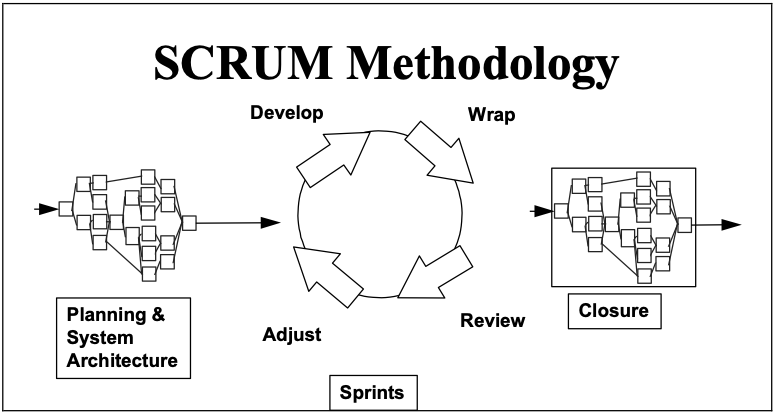
\includegraphics[scale=0.4]{images/planning/scrum_phases}}
\end{figure}

\section{Tasks and scheduling}
To accomplish the project objectives the following tasks are proposed:
\begin{itemize}
    \item \textbf{[T1]} Study of the state of the art of the problem.
    \begin{itemize}
        \item \textbf{[T1.1]} Study of the Spanish electrical market, understanding the agents, processes and variables that conform it.
        \item \textbf{[T1.2]} Review of the literature about time series analysis and forecasting, understanding the different techniques and tools that can be useful to meet our objectives.
    \end{itemize}
    \item \textbf{[T2]} Find the necessary data to perform the study.
    \begin{itemize}
        \item \textbf{[T2.1]} Download the data from the internet, either manually or automatically through an API.
        \item \textbf{[T2.2]} Preprocess and study the downloaded data.
    \end{itemize}
    \item \textbf{[T3]} Perform the analysis over the data.
    \begin{itemize}
        \item \textbf{[T3.1]} Forecast prices in the short, medium and long terms.
        \item \textbf{[T3.2]} Study which variables are affecting the electricity price on the short, medium and long term.
    \end{itemize}
    \item \textbf{[T4]} Document the results in this report.
\end{itemize}

It is important to allocate a reasonable time frame for each task.
This project is framed in a 6 credit Master Thesis which means 150 hours of work, we will split this hours through 9 sprints, of two weeks each. That means 9 hours of work per week approximately. The initial scheduling is exposed in the Gantt diagram in Figure \ref{fig:planning-gantt}.

\begin{figure}[H]
\centering
    \caption{Gantt diagram with project task scheduling.}
    \label{fig:planning-gantt}
    \fbox{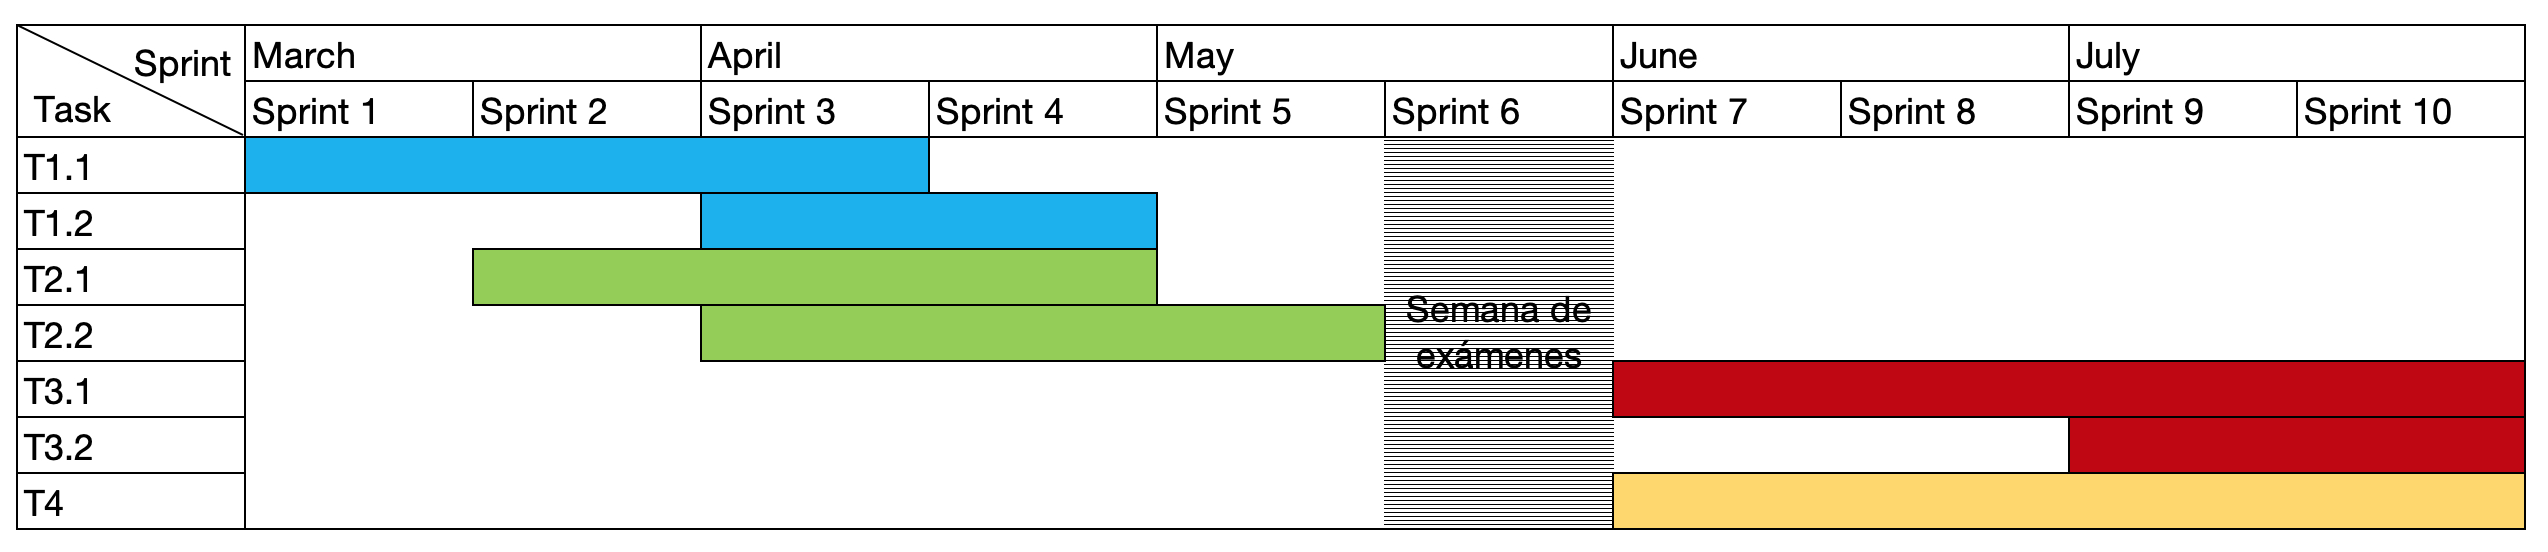
\includegraphics[scale=0.33]{images/planning/planning_gantt}}
\end{figure}
\chapter{State of the art}
\label{ch:state-of-the-art}
Time series are a type of data that indicate how things change over time. They are different from other types because time is a fundamental dimension on them, being data order as important as the data per se. That's why analyzing and forecasting time series is more challenging and extra considerations should be taken into account. \cite{lazzeri2020machine}

\section{Time series components}
The three components that conform them are:
\begin{itemize}
    \item Trend component ($T_t$): Defined as the long term movement in a time series. It can be constant, increasing or decreasing in time.
    \item Seasonal component ($S_t$): Periodic fluctuations in the series that normally happen in a period of less than a year. Weather seasons or social conventions are examples of what produces this seasonality.
    \item Cyclic component ($C_t$): Recurrent fluctuations that appear in the series but don't have a fixed length. An example of this is a business cycle, whose duration is not known a priori.
    \item Remainder component ($R_t$): Unpredictable variations that can not be explained by the other three.
\end{itemize}

They can be combined in an additive way ($y_t = S_t + C_t + T_t + R_t$), a multiplicative one ($y_t = S_t \times C_t \times T_t \times R_t$) or a combination of both ($y_t = S_t \times C_t + T_t + R_t$, $y_t = S_t + C_t + T_t \times R_t$\ldots). The additive decomposition is more adequate when the degree of variation in the components doesn't seem to change with the level of the time series. Otherwise, is more recommended to apply a multiplicative one.  \cite{hyndman2018forecasting,lazzeri2020machine}

\subsubsection{Stationarity}
A very important concept in time series is stationarity.
A stationary time series is one whose properties does not change with time, with the moment in which the series is observed. If some trend or seasonality is present, it doesn't hold.

Usually, an stationary time series will have no predictable patterns in the long term. Nevertheless, a cyclic behaviour with no trend nor seasonality is stationary.

One way of detecting stationarity is by generating ACF plots, like the one in Figure \ref{fig:solar-acf}. They also are useful to detect cycles in the series.


\section{Forecasting}
In \cite{hyndman2018forecasting}, the author explains that "forecasting is about predicting the future as accurately as possible, given all the information available, including historical data and knowledge of any future events that might impact the forecasts".
Selecting an adequate forecasting method will depend on the characteristics of the time series, using simpler or more advanced methods.

\subsection{Simple methods}
In some situations they can be really effective. Some of these methods are: \cite{hyndman2018forecasting}
\begin{itemize}
    \item \textbf{Average method:} Forecast with the mean of the historical data. A very popular variation of this technique is the Moving Average (MA) method, in which the mean is computed not over the complete historical series but over the K more recent points.
    \item \textbf{Naïve method:} Forecast with the last observation of the historical data.
    \item \textbf{Drift method:} A modification of the previous technique where forecasts increase or decrease over time.
\end{itemize}

\subsection{Classical methods}
These methods were developed some decades ago and are based in statistics. They have been the de facto standard to forecast time series until the creation of more advanced methods. Some of them are: \cite{lazzeri2020machine, hyndman2018forecasting}
\begin{itemize}
    \item \textbf{Exponential smoothing (ETS):} Uses the MA method, assigning higher weights to more recent values and lower weights to those which are more distant in time. Combines Error, Trend and Seasonality components to model the series.
    \item \textbf{Auto Regressive Integrated Moving Average (ARIMA):} Combines an autoregressive model, in which a linear model is trained using as predictors the lagged values of the variable, with a moving average and integration. In the moving average, instead of forecasting using lags of the actual variable, past forecasting errors are used as predictors. The integration step is in charge of making the time series stationary.
\end{itemize}

\subsection{Advanced methods}
The development in Machine Learning (ML) also arrived to time series. We can use our favourite models as Random Forest, k-Nearest Neighbours or even LSTM to forecast the future. But data has to be structured in a particular way, using lags so these models can capture autocorrelation.

\section{Predictor's influence}
%When forecasting (and predicting in general) it is important to build a model that adequately captures the underlying patterns of data. This will lead to accurate and strong predictions.
%
%But in many cases it is also important to understand how data is affecting the model. Which variables are more important in the prediction? How and why? This is an issue that model interpretability attempts to solve.
TODO




sktime \cite{DBLP:journals/corr/abs-1909-07872}
pmdarima \cite{pmdarima}
scikit-learn \cite{scikit-learn}
SHAP package \cite{shap-package}

\chapter{The Spanish electricity market}
In this section we briefly describe how the wholesale electricity market works in Spain.
In 1998, the current regulation came into operation, replacing the previous system in which Red Eléctrica de España (REE) and the Ministry of Industry and Energy entirely planned their transactions.

It allowed the private sector to freely plan the construction of generation plants and the possibility of bidding energy prices, and created the figure of energy supplier (being the consumer able to choose one).
Distribution of energy remained regulated by the government, who assigns this task to a unique company per region. \cite{mercado-electrico-mincotur}

The wholesale electricity market differs from the retail market. In the former generators sell energy to suppliers, while in the latter suppliers sell energy to consumers. Different agents participate in both, and they are regulated by different rules, being more flexible in the retail market.

\section{Main agents}
Different agents conform this complex system. Each one is in charge of a specific task:\cite{mercado-electrico-endesa, organismos-reguladores-holaluz}

\begin{itemize}
    \item \textbf{Generators} produce energy and should build, operate and maintain the power plants.
    \item \textbf{Transporters} take the energy from the power plants to the distribution network, building and maintaining the transport network. This network operates in high voltage, making transmission through long distances more efficient.
    \item \textbf{Distributors} extract the energy from the transport network and supply it to the final consumers. They are in charge of building and maintaining the distribution network.
    \item \textbf{Suppliers} buy the energy to generators and sell it to final consumers.
    \item \textbf{Regulators} are in charge of legislating (government administration) and ensuring effective competition (Comisión Nacional de los Mercados y la Competencia, CNMC) in the energy market.
    \item There exist two \textbf{operators}, the market operator and the system operator. The former (Operador de Mercado Ibérico de Energía, OMIE) manages the day-ahead and intraday electricity markets. The latter (Red Eléctrica de España, REE) ensures the system stability, checking that generation and consumption are balanced every time as energy can't be stored in large scale, preventing lack of supply or overload on the power grid. Both operators should work closely, so they can face adequately to problems in the system.
\end{itemize}

\section{The electricity price}
The main goal of this Thesis is to study electricity market prices.
These are the prices which supplying companies pay for the energy, and not the final price each consumer pays when using, for example, the Precio Voluntario Pequeño Consumidor (PVPC) tariff, which also includes regulated costs and taxes. \cite{mercado-electrico-xataka}

The prices for next day are fixed in the electricity market or pool, which happens every day at 12 pm.
On it, suppliers make their purchase bids, which are ordered from lower to higher in the supply curve (green curve in Figure \ref{fig:supply-demand-curves})
On the other hand, generators make their sell bids which are ordered from higher to lower in the demand curve (blue curve in Figure \ref{fig:supply-demand-curves}).

\begin{figure}[H]
\centering
    \caption{Energy supply and demand curves in the wholesale market. \cite{curva-oferta-demanda}}
    \label{fig:supply-demand-curves}
    \fbox{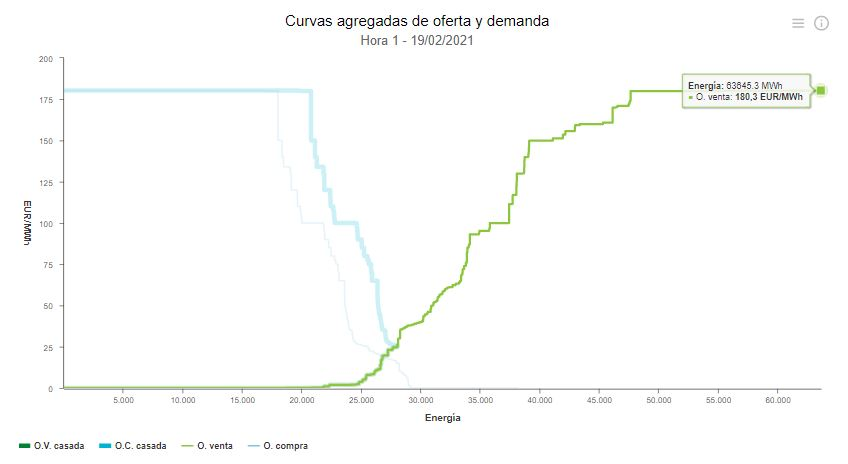
\includegraphics[scale=0.6]{images/supply-demand-curves.jpeg}}
\end{figure}

The point where the two curves intersect defines the price at which energy will be sold. On the left of this intersection appear the transactions that will take place, while those on the right will not be materialized, as the generators ask for more money than what suppliers are willing to pay.
All the sold electricity will be available at that intersection price, the generators will receive that price even if they bid for less.

These characteristics are what define a marginal pricing market.
This process will be repeated for each hour of the following day, having a total of 24 different prices.

This variable will be obtained both from ESIOS (short term) and OMIE (long term): both data sources contain the same information, as prices are built in a regulated basis as explained in the previous paragraphs. The data acquired goes from 01-1998 to 03-2023, in an hourly fashion.

Let's visually analyze the data in Figure \ref{fig:spot-price-series}. On an hourly scale, the author appreciates some cyclicity happening every 12 hours, something that can be confirmed in the ACF plot.
Concretely, peaks in price appear at the early morning and in the evening.
During the night and late morning the price goes down: this could be due to our daily routines, as we consume less energy while we sleep or while we are working.
Nevertheless, we will know more about this in the future sections, when we study the predictor's importance.
On a monthly scale the author doesn't find cyclicity. But it is interesting to mention the peak in prices between 2021 and 2023 due to the war in Ukraine, as Europe is very dependent of fossil fuels imported from Russia \cite{lopez2022geopolitica}.

\begin{figure}[H]
\centering
    \begin{subfigure}{.45\textwidth}
        \centering
        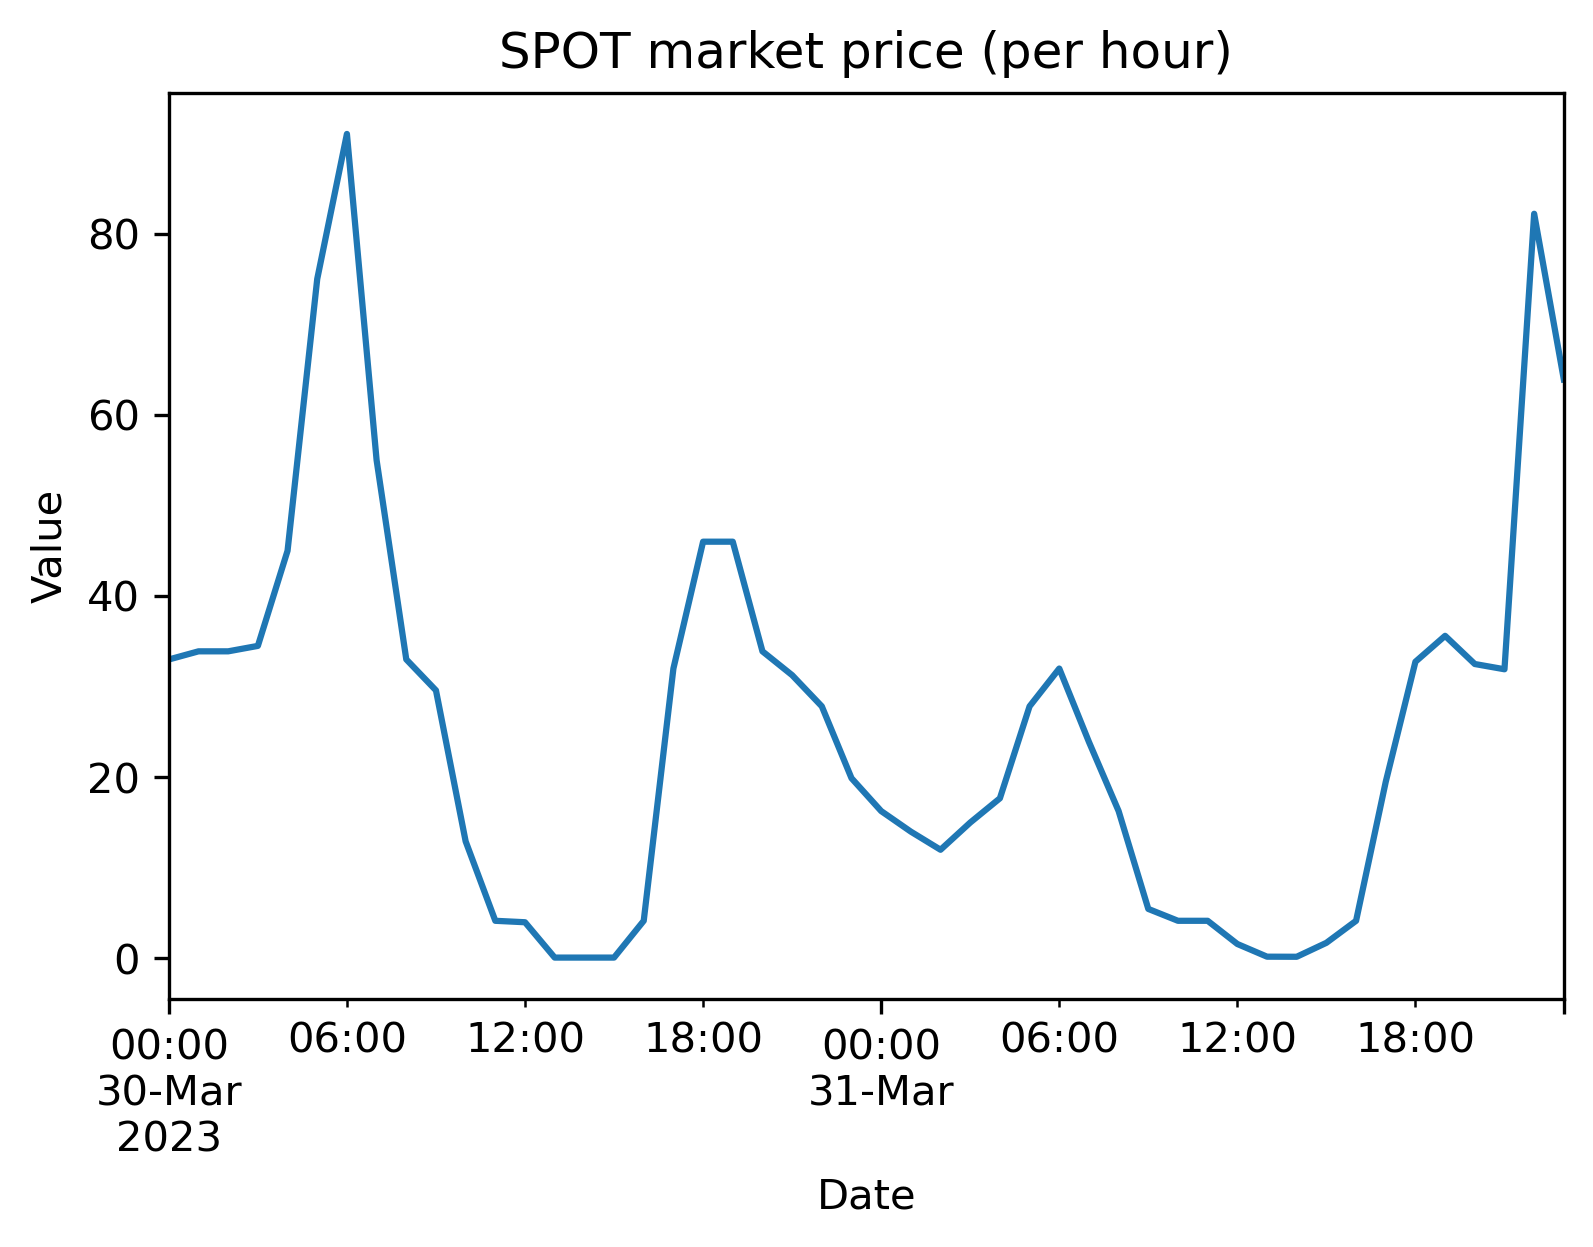
\includegraphics[width=1\linewidth]{images/variable_analysis/esios_spot_h_48}
        \caption{Per hour, 48 hours window.}
    \end{subfigure}
    \begin{subfigure}{.45\textwidth}
        \centering
        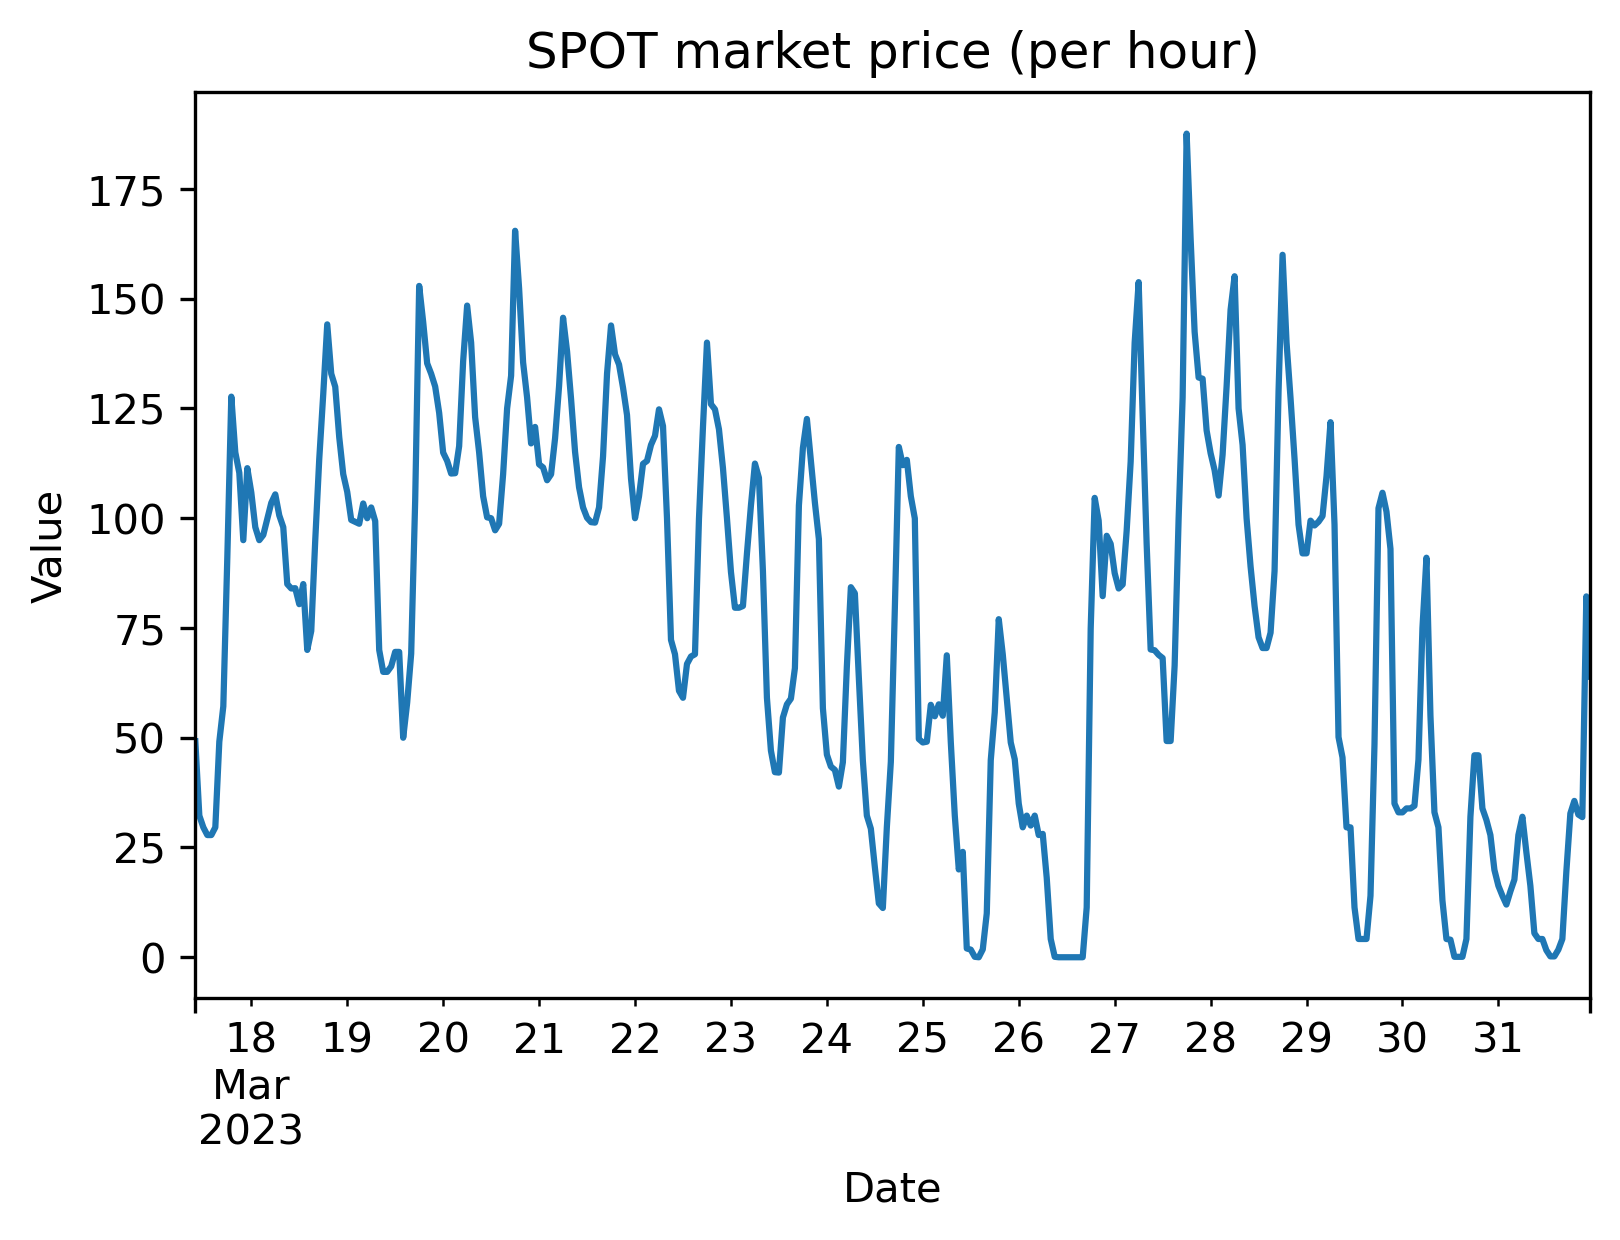
\includegraphics[width=1\linewidth]{images/variable_analysis/esios_spot_h_350}
        \caption{Per hour, 350 hours window.}
    \end{subfigure}
\end{figure}

\begin{figure}[H]\ContinuedFloat
    \begin{subfigure}{.45\textwidth}
        \centering
        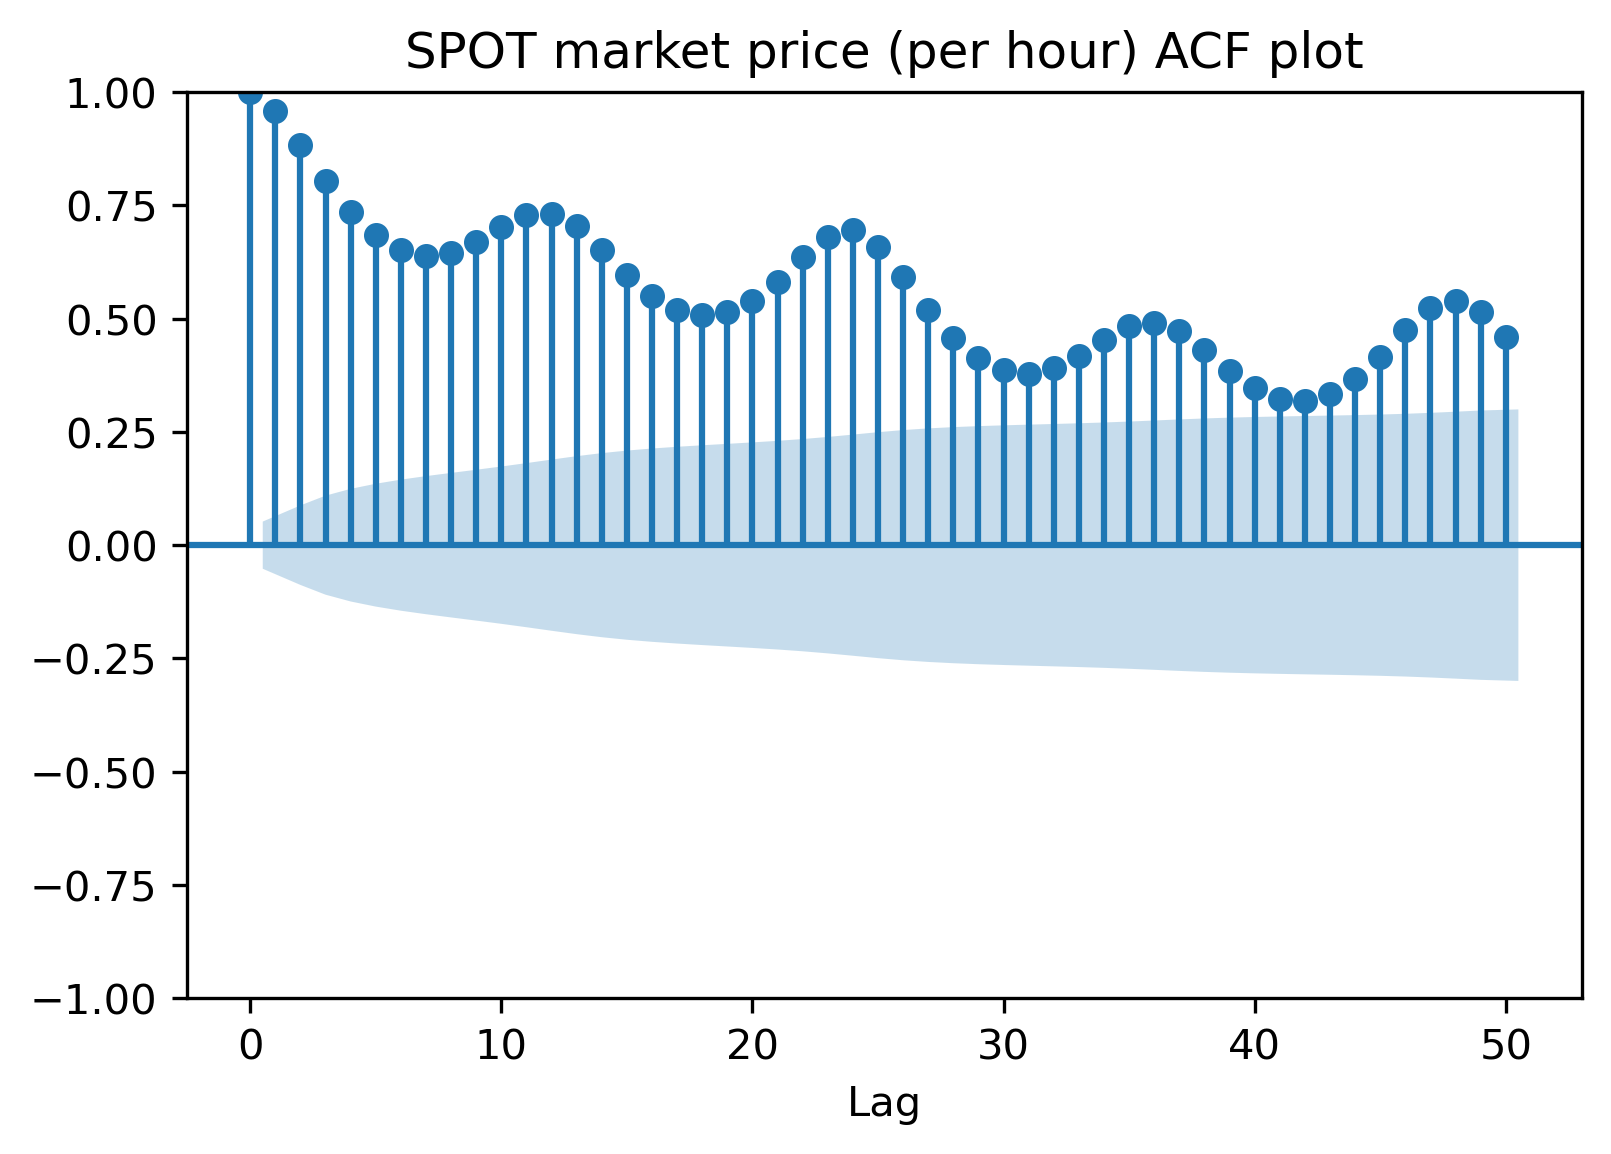
\includegraphics[width=1\linewidth]{images/variable_analysis/esios_spot_h_acf}
        \caption{ACF plot with 50 lags.}
    \end{subfigure}
    \begin{subfigure}{.45\textwidth}
        \centering
        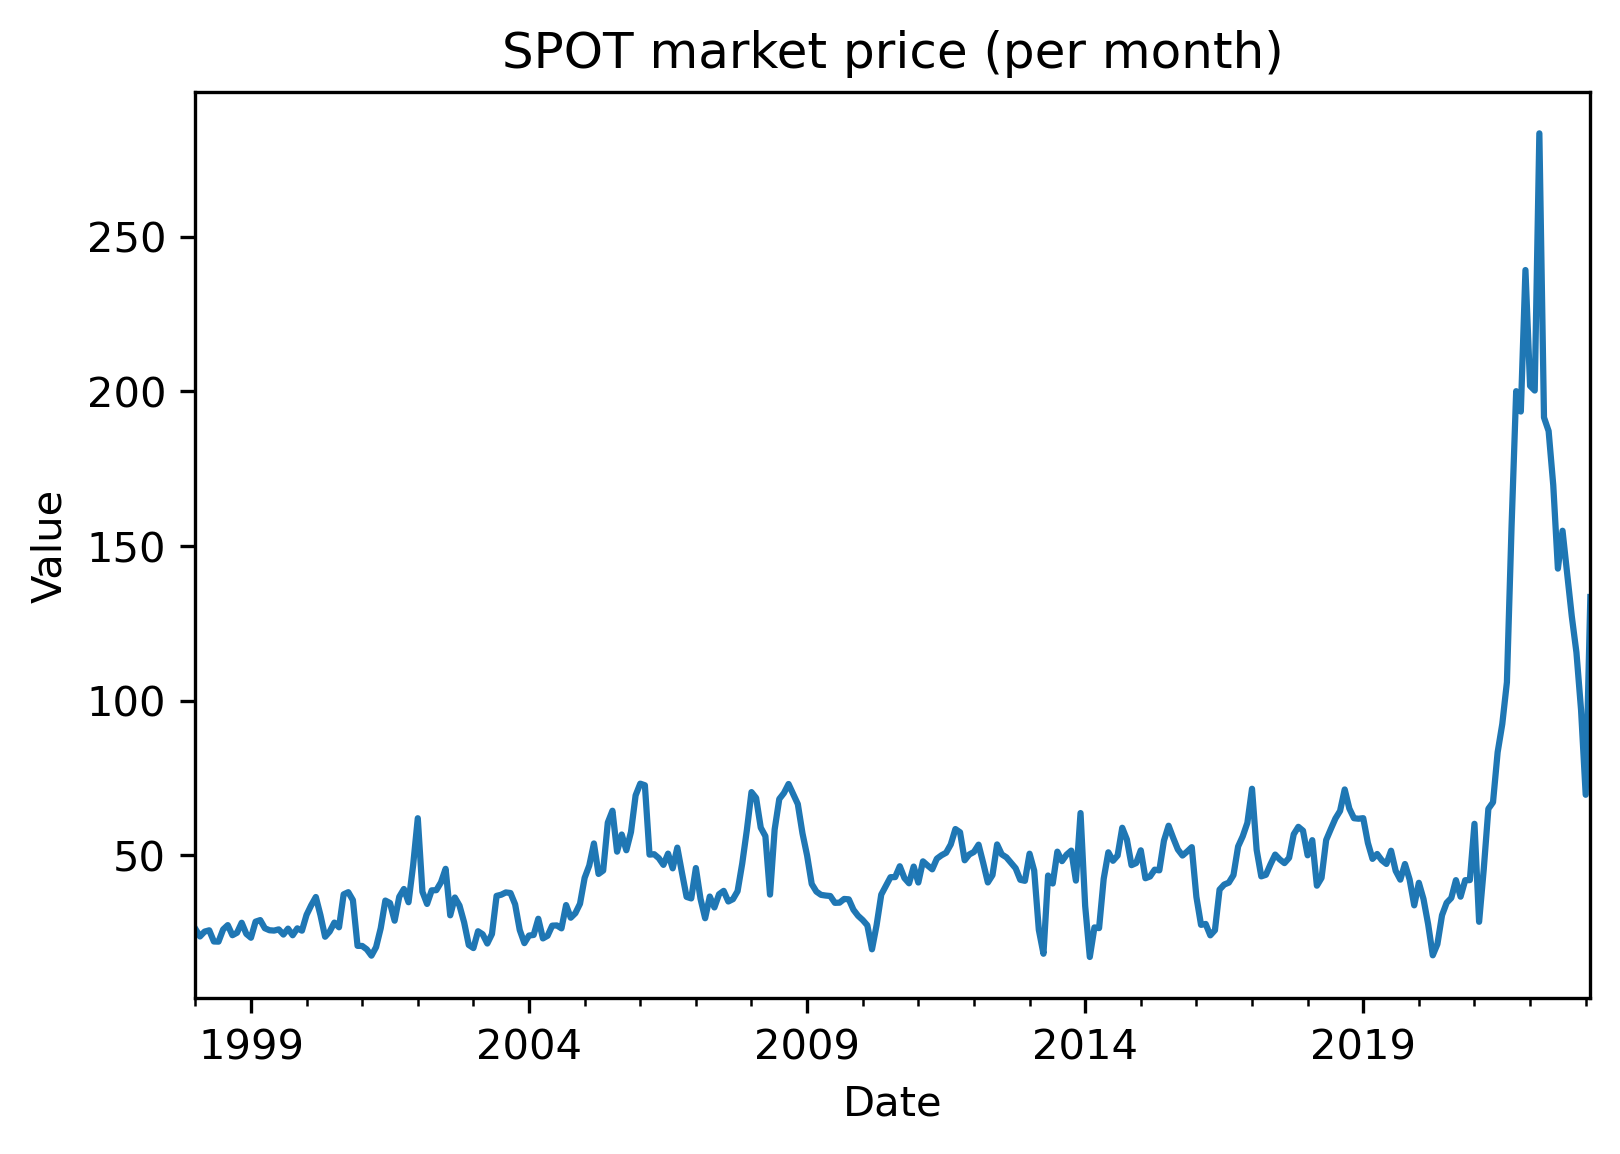
\includegraphics[width=1\linewidth]{images/variable_analysis/esios_spot_m_omie_all}
        \caption{Aggregated by month.}
    \end{subfigure}

    \caption{Electricity market SPOT price curves analysis.}
    \label{fig:spot-price-series}
\end{figure}

\section{Variables affecting the electricity price}
As the price is built in the free market, defining a priori the variables that influence it is difficult.
Many factors can affect its value, even companies strategic decisions that can't be predicted, but there are some variables that could fit in the equation that will be described in the following subsections. \cite{mercado-electrico-periodico-energia, mercado-electrico-cambio-energetico}

\subsection{Demand}
The energy consumption can affect the price, specially in a marginal pricing market.
As generation bids are ordered in the supply curve from cheaper to expensive, if the demand is high the intersection point will probably move to the right leading to a higher price.
The measured demand curves have been downloaded from ESIOS, obtaining data from 01-2014 to 03-2023. The granularity they originally have is of one reading every 10 minutes, but the author has aggregated this into hourly measurements.

If we study the plots in Figure \ref{fig:demand-series} we find how there is cyclicity at a daily level, there are repeating patterns each 24 hours, which makes sense due to people daily routines. There is also weekly cyclicity, existing higher consumption during the work days than during the weekends: this could be related with industry energy demand. It is also happening at yearly and half-yearly levels.

\begin{figure}[H]
\centering
    \begin{subfigure}{.435\textwidth}
        \centering
        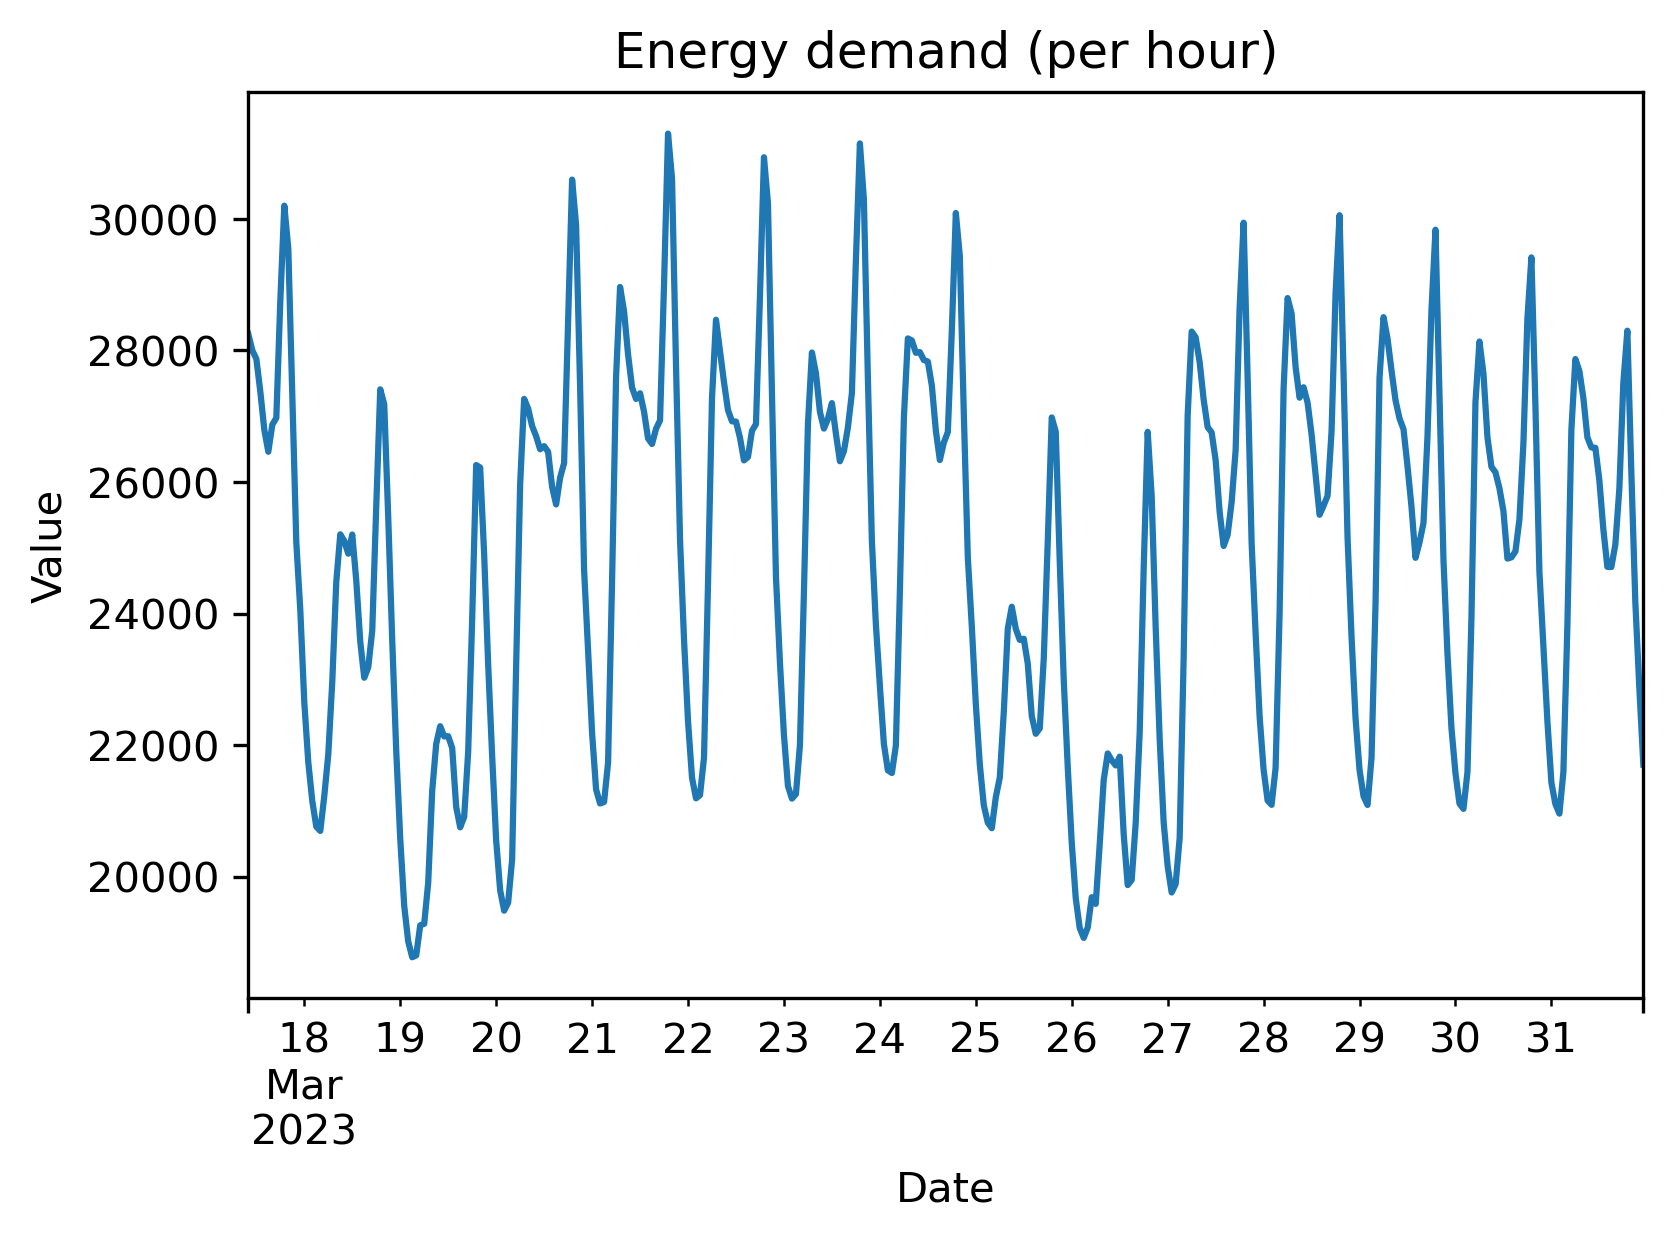
\includegraphics[width=1\linewidth]{images/variable_analysis/esios_demand_h_350}
        \caption{Per hour, 350 hours window.}
    \end{subfigure}
    \begin{subfigure}{.45\textwidth}
        \centering
        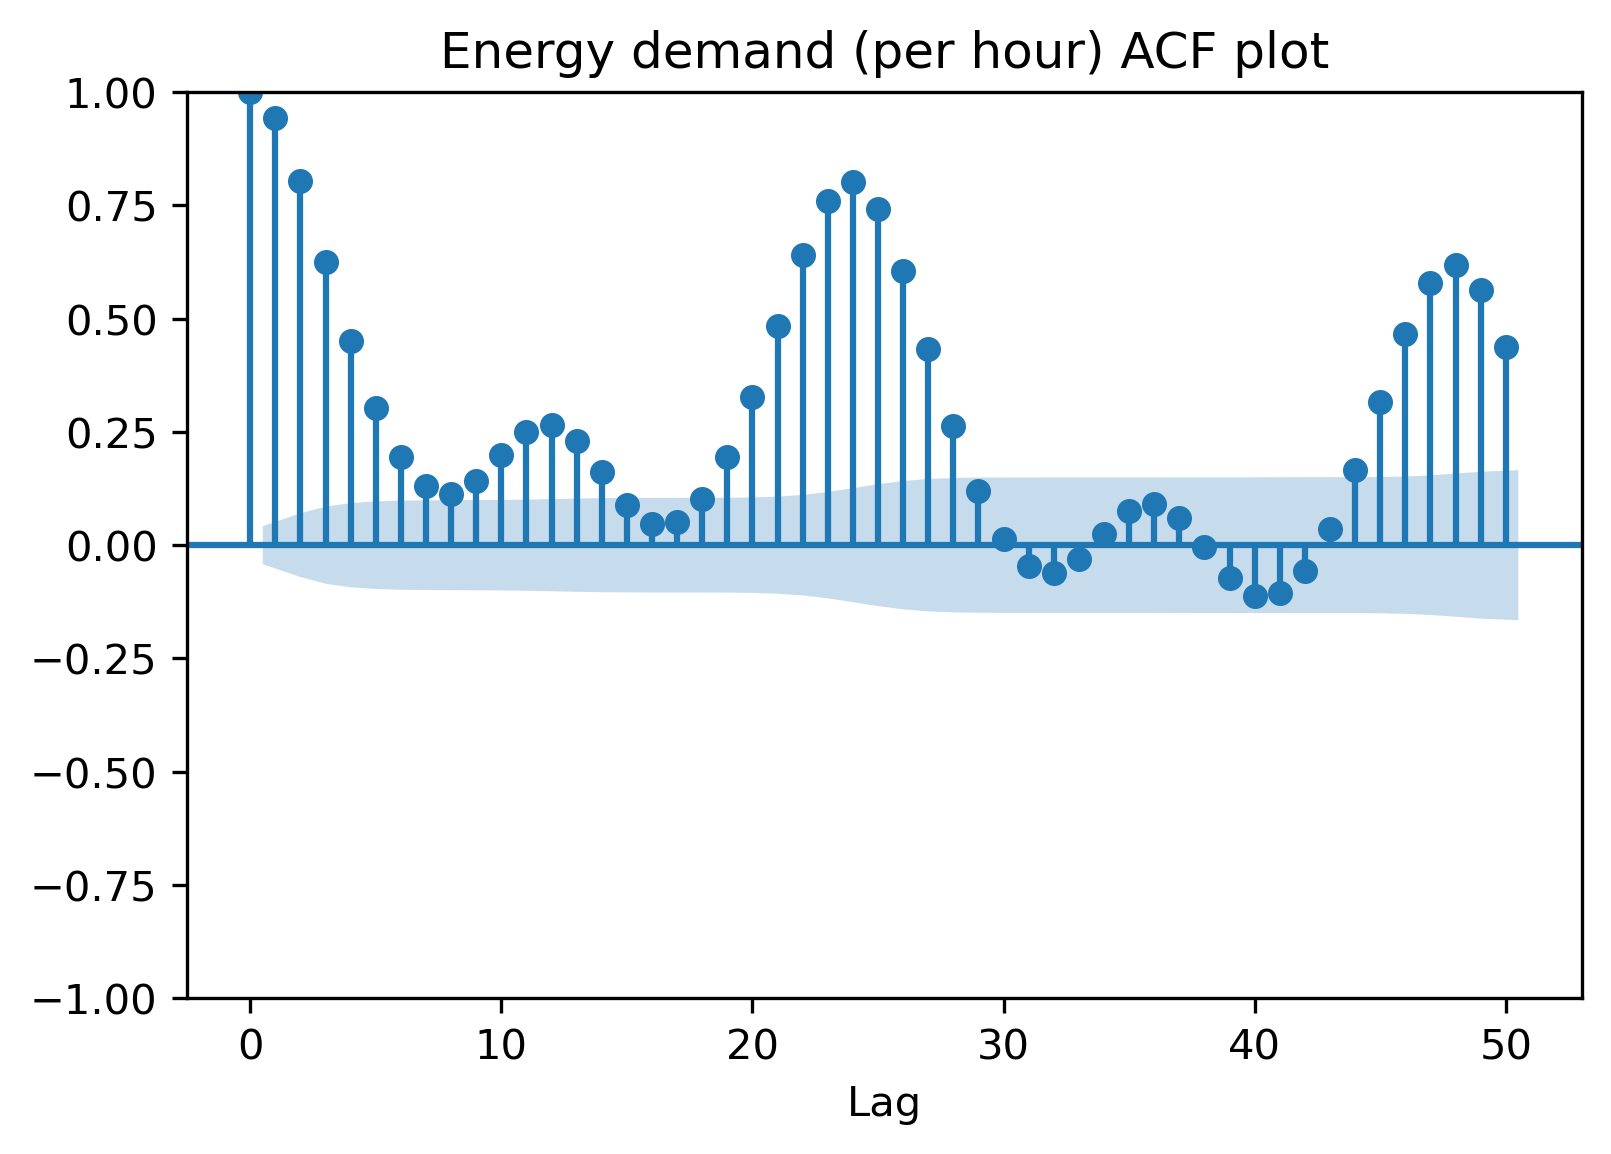
\includegraphics[width=1\linewidth]{images/variable_analysis/esios_demand_h_acf}
        \caption{Per hour, ACF plot.}
    \end{subfigure}
\end{figure}

\begin{figure}[H]\ContinuedFloat
    \begin{subfigure}{.44\textwidth}
        \centering
        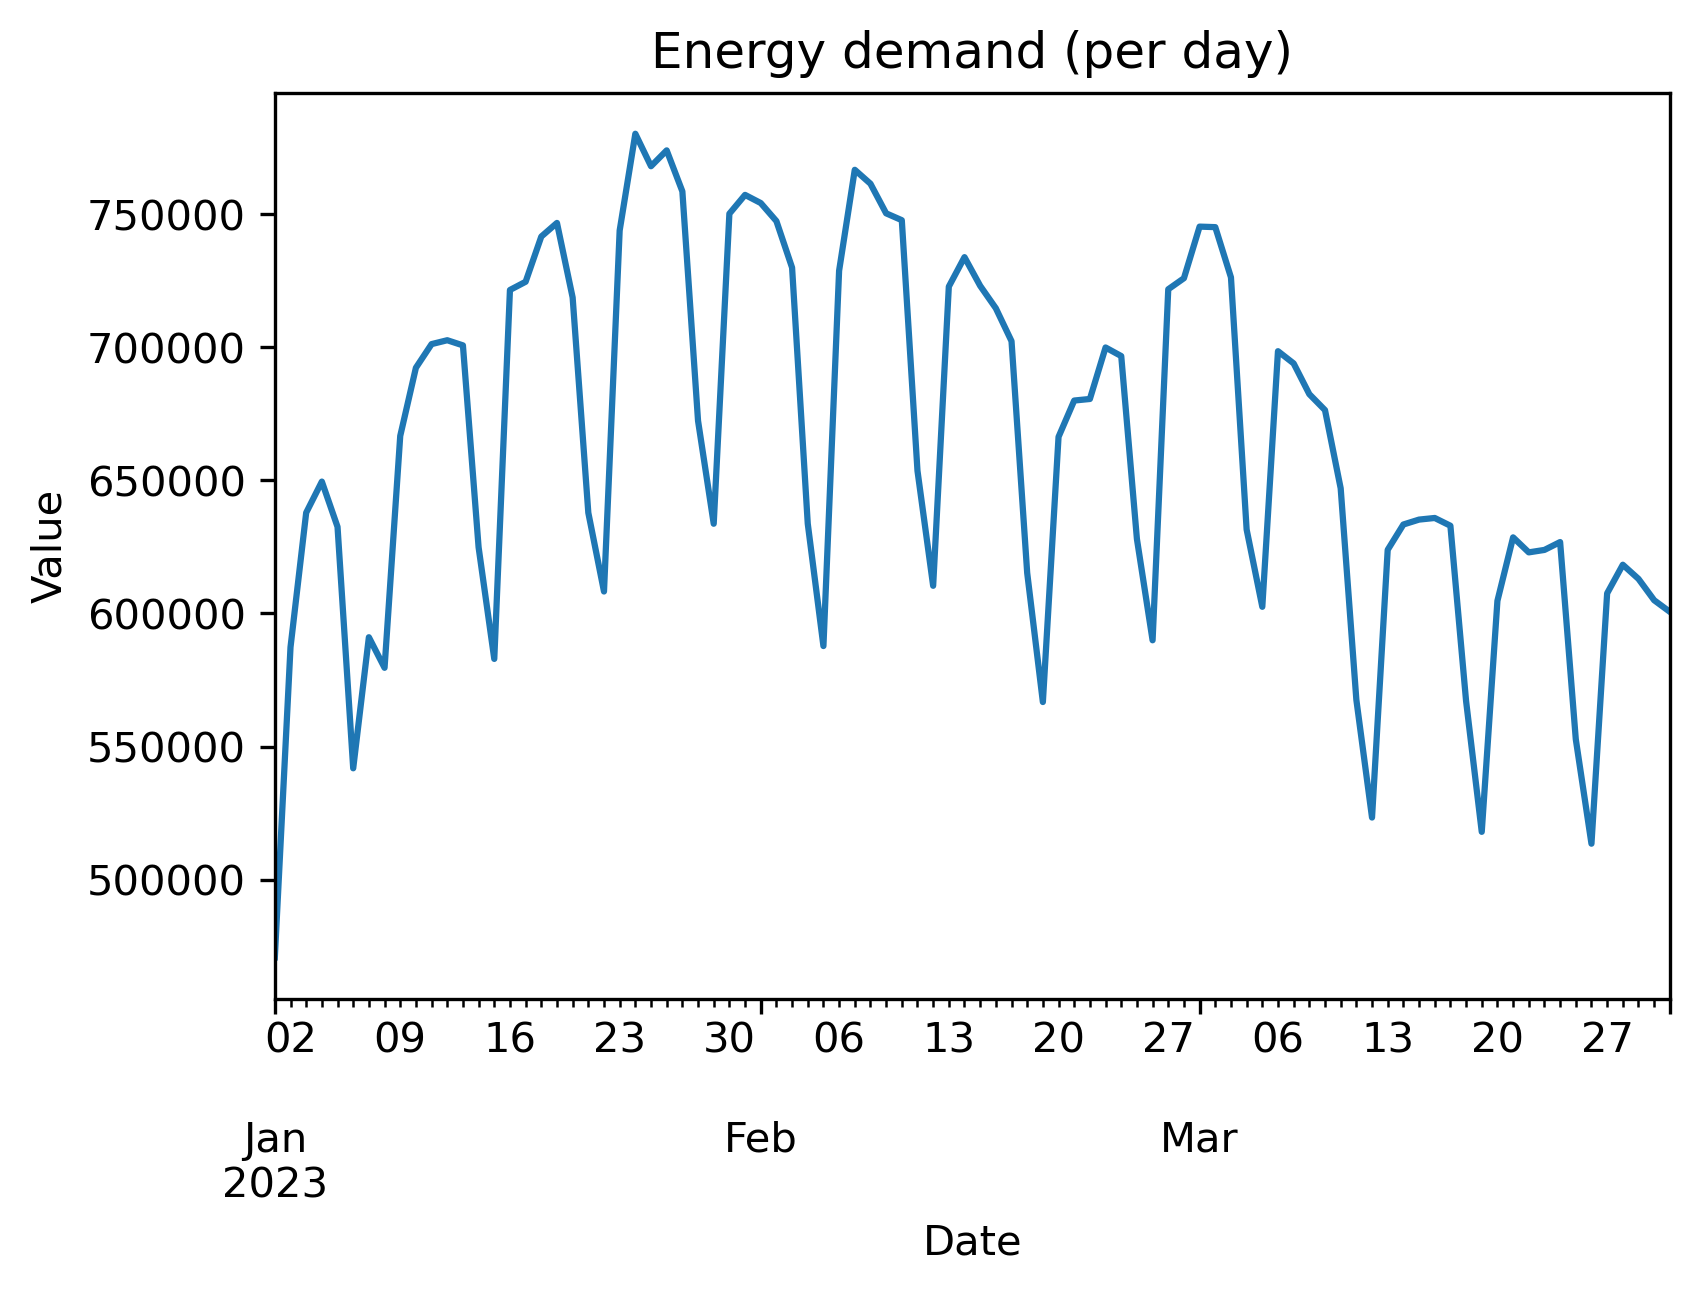
\includegraphics[width=1\linewidth]{images/variable_analysis/esios_demand_d_90}
        \caption{Aggregated by day, 90 days window.}
    \end{subfigure}
    \begin{subfigure}{.45\textwidth}
        \centering
        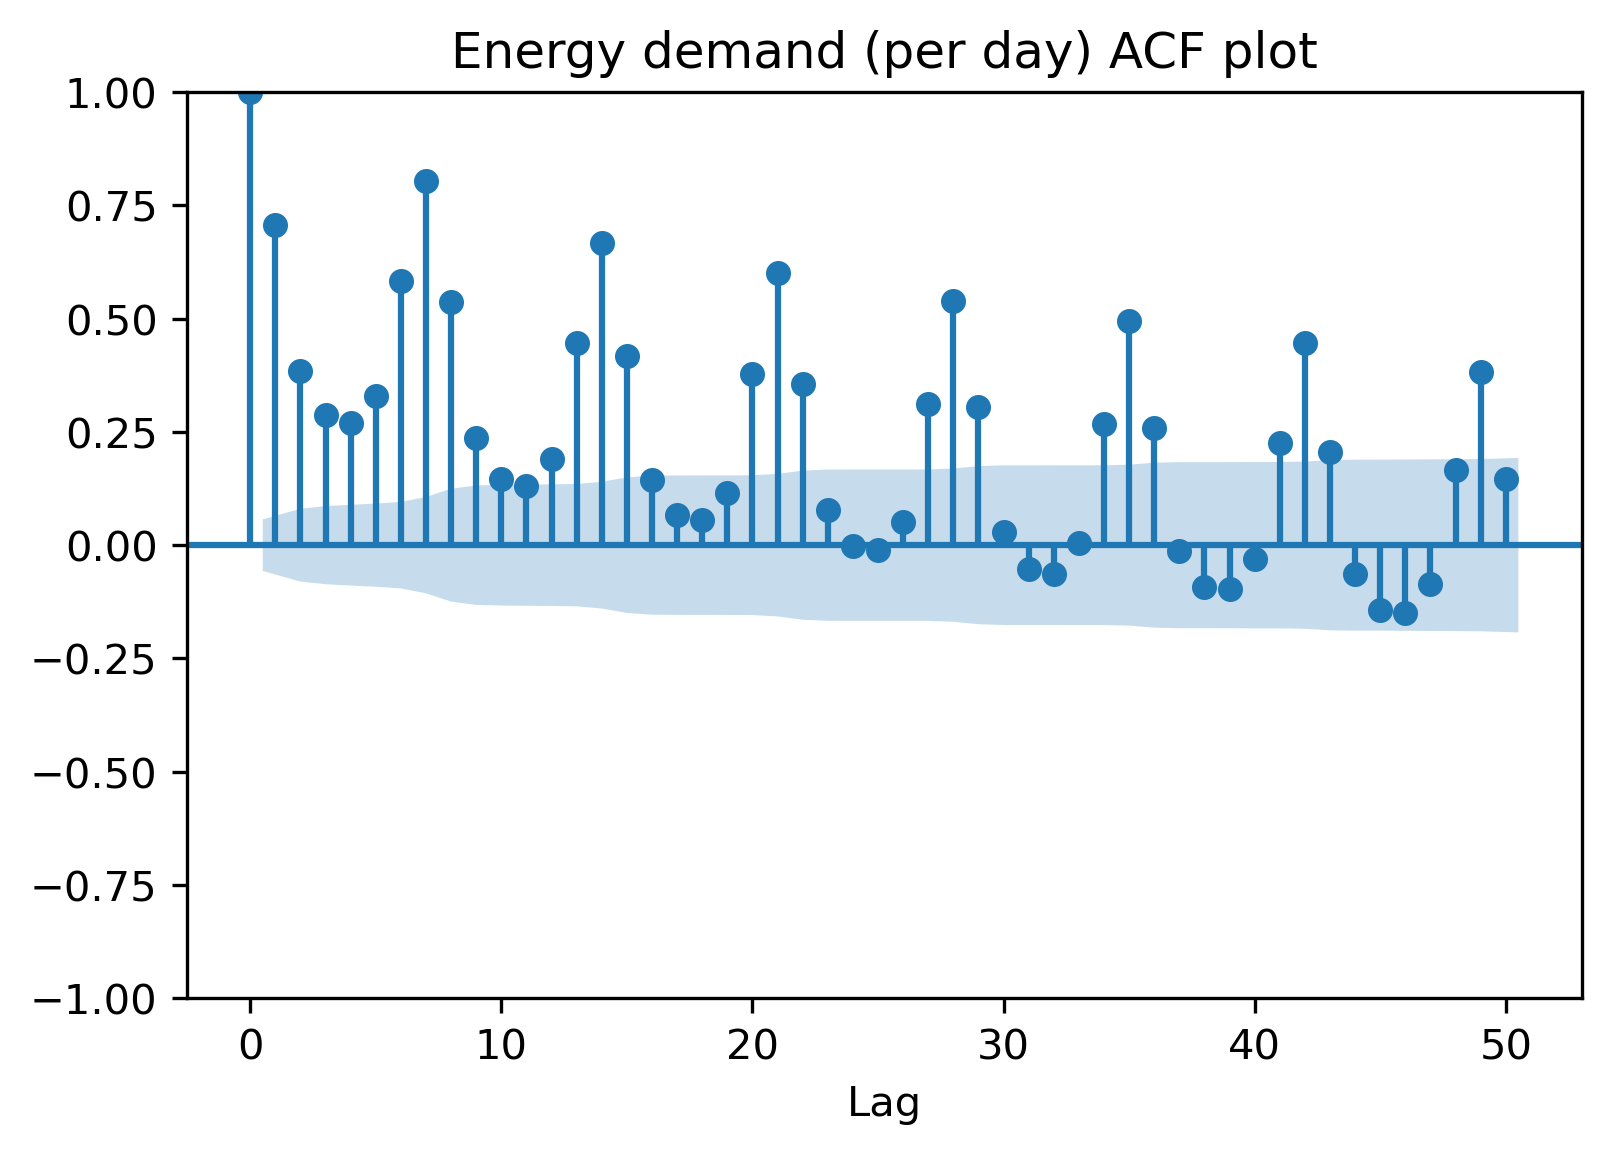
\includegraphics[width=1\linewidth]{images/variable_analysis/esios_demand_d_acf}
        \caption{Per day, ACF plot.}
    \end{subfigure}
\end{figure}

\begin{figure}[H]\ContinuedFloat
    \begin{subfigure}{.43\textwidth}
        \centering
        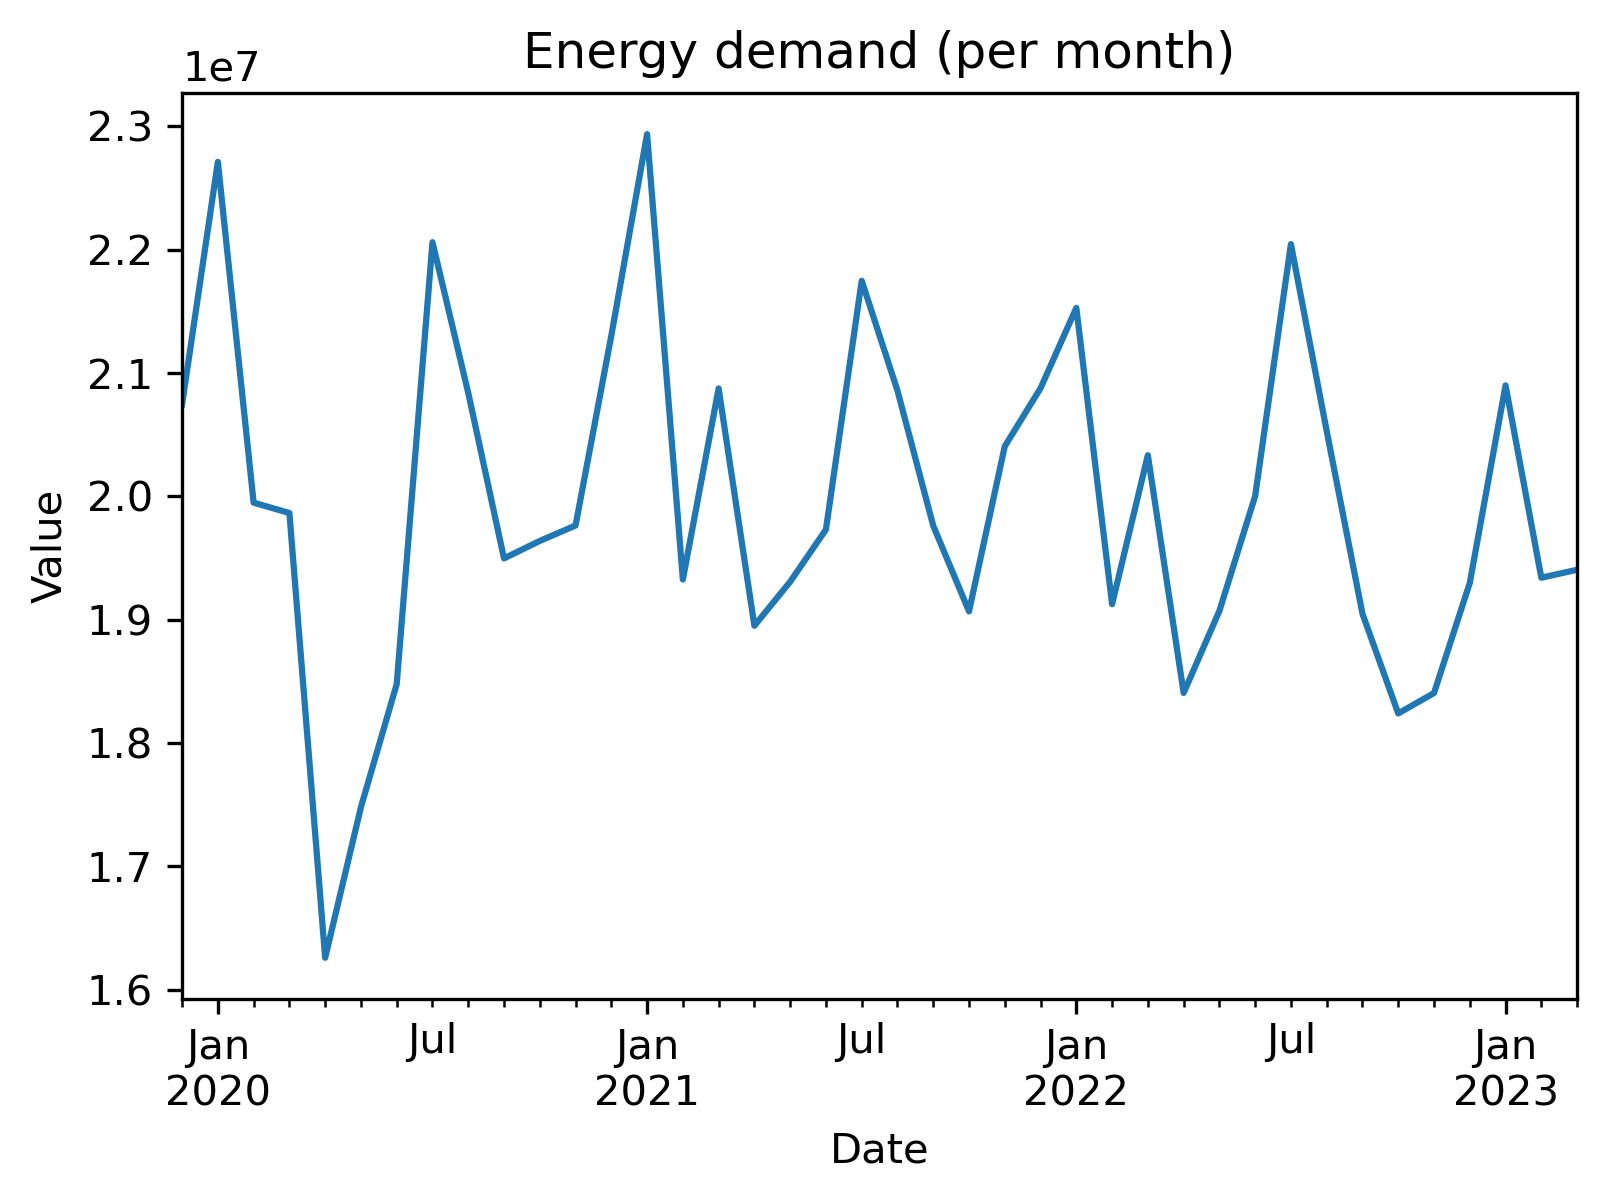
\includegraphics[width=1\linewidth]{images/variable_analysis/esios_demand_m_40}
        \caption{Aggregated by month, 40 months window.}
    \end{subfigure}
    \begin{subfigure}{.45\textwidth}
        \centering
        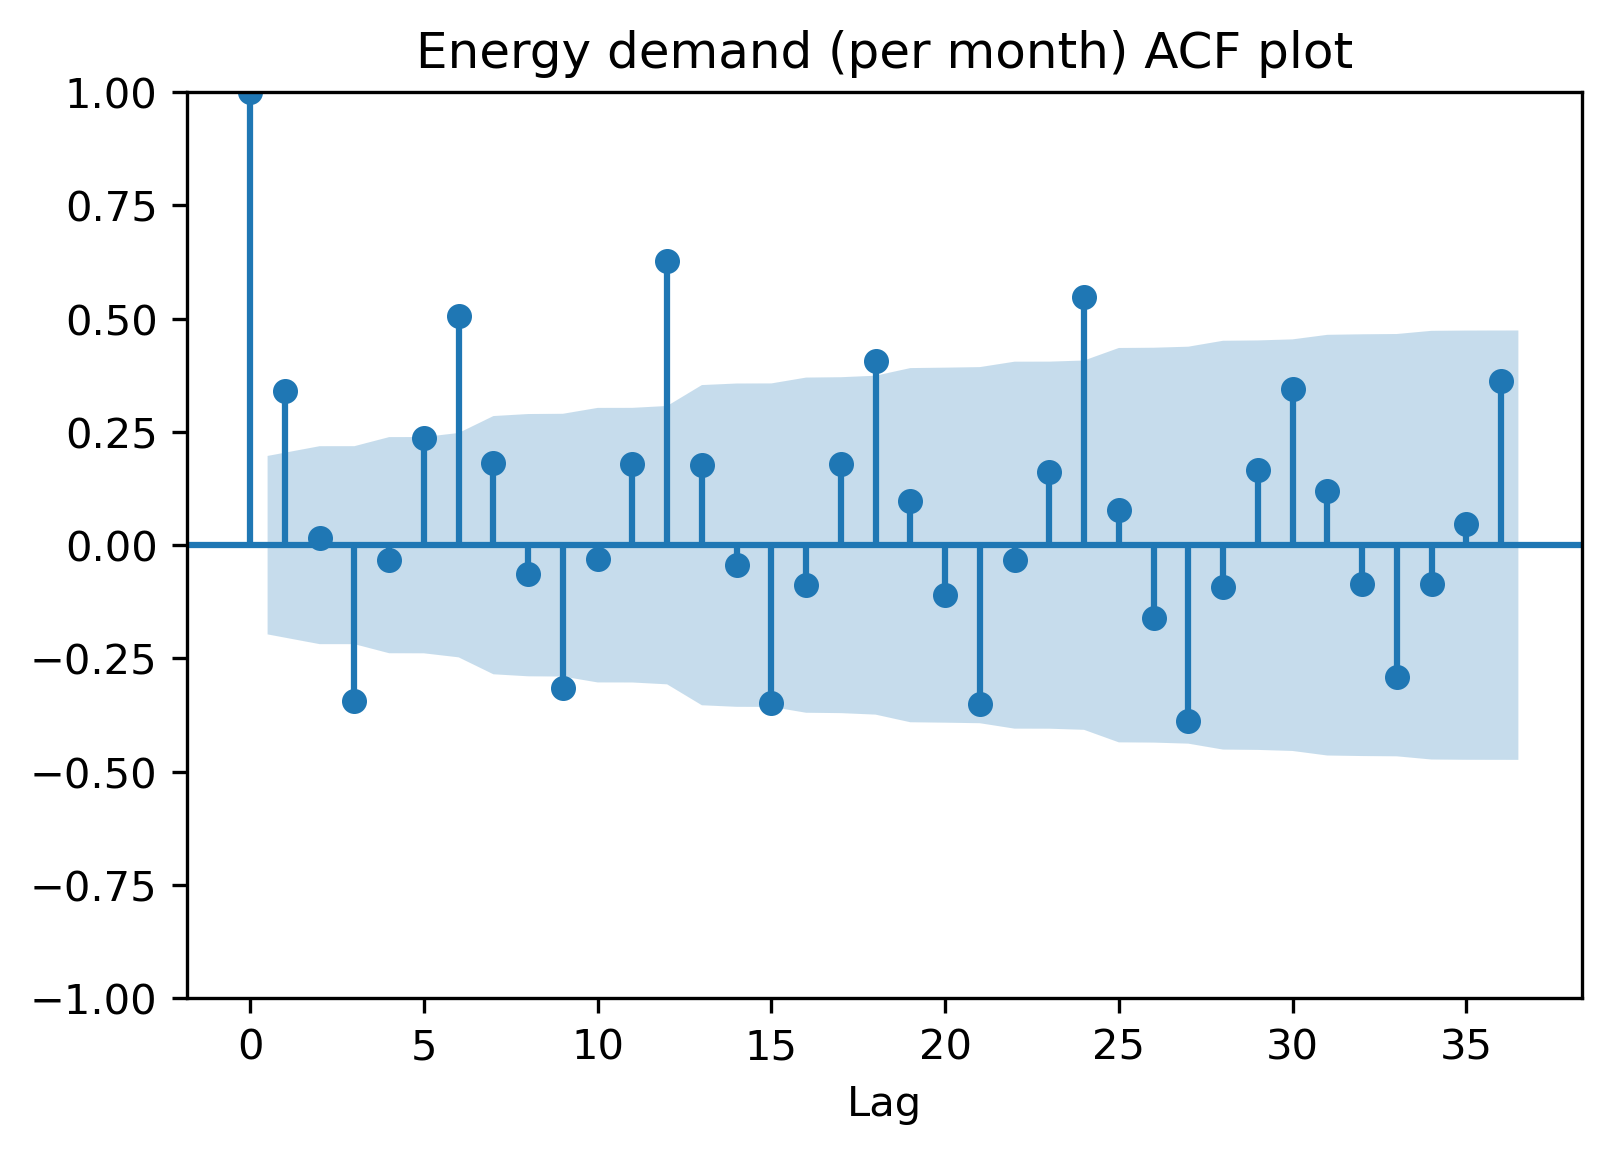
\includegraphics[width=1\linewidth]{images/variable_analysis/esios_demand_m_acf}
        \caption{Per month, ACF plot.}
    \end{subfigure}

    \caption{Electricity demand curves analysis.}
    \label{fig:demand-series}
\end{figure}

\subsection{Generation}
Energy generation involves the transformation of sources of primary energy into electricity.
The generation technologies differ in the way they produce the energy and in the primary energy they use for this task, each having different building and operation costs, technical characteristics and impact in the environment. \cite{subasta-electrica-totalenergies}

Demand and total generation are correlated, as the system operator is in charge of maintaining a balance between both.
There are generation technologies that always bid for a low price, even zero, as the nuclear: this is because a nuclear plant can't stop working, so it is always interested in selling the energy no matter the price.
Other as wind energy are also sold at a low price but not as low, because even though it is a cheap energy (the fuel is the own wind), the more you use a turbine the more maintenance it needs.
As it can be stopped, sometimes it is more adequate to do that than selling for zero.
Finally, technologies that tend to set the price of electricity are those using commodities, as combined cycles.

All the generation data has been downloaded from ESIOS in an hourly fashion.
We have downloaded generation data of the following technologies:
\begin{itemize}
    \item \textbf{Wind:} Existing yearly and half-yearly cyclicities have been found. This could make sense as wind may depend on temperature through the year. There is also a positive trend in the last years of wind energy generation.
    \item \textbf{Hydropower:} Strong daily cyclicity, with generation peaks in the hours with higher energy demand (Figures \ref{fig:hydro-series} and \ref{fig:hydro-acf}). There seems to be some weekly cyclicity but not very strong. The same happens in a yearly level.
    \item \textbf{Solar:} Really high daily cyclicity (Figure \ref{fig:solar-acf}). Cyclicity also in a yearly fashion, with a positive trend in the solar energy generation in the previous years (Figure \ref{fig:solar-series}).
    \item \textbf{Nuclear:} In the short term it is a very stable energy technology, with not many generation changes between nearby hours, see Figure \ref{fig:nuclear-series}. Maybe some cycles appear in a yearly and half-yearly fashion, but they are not very clear. There is no trend in the long term for the generation with this technology.
    \item \textbf{Combined cycles:} This technology, powered by gas, uses the combustion to move turbines. Apart, the residual heat is used to heat water and move other turbines, increasing generation efficiency. There exists some cyclicity in half-daily, daily and weekly horizons.
    \item \textbf{Coal:} This raw material has been a very popular fuel in thermal power plants, but in the previous years its use has decreased a lot due to how pollutant is. As can be seen in Figure \ref{fig:coal-series}, the use of coal as generation fuel has decreased a lot in the last years.
\end{itemize}

\begin{figure}[H]
\centering
    \begin{subfigure}{.43\textwidth}
        \centering
        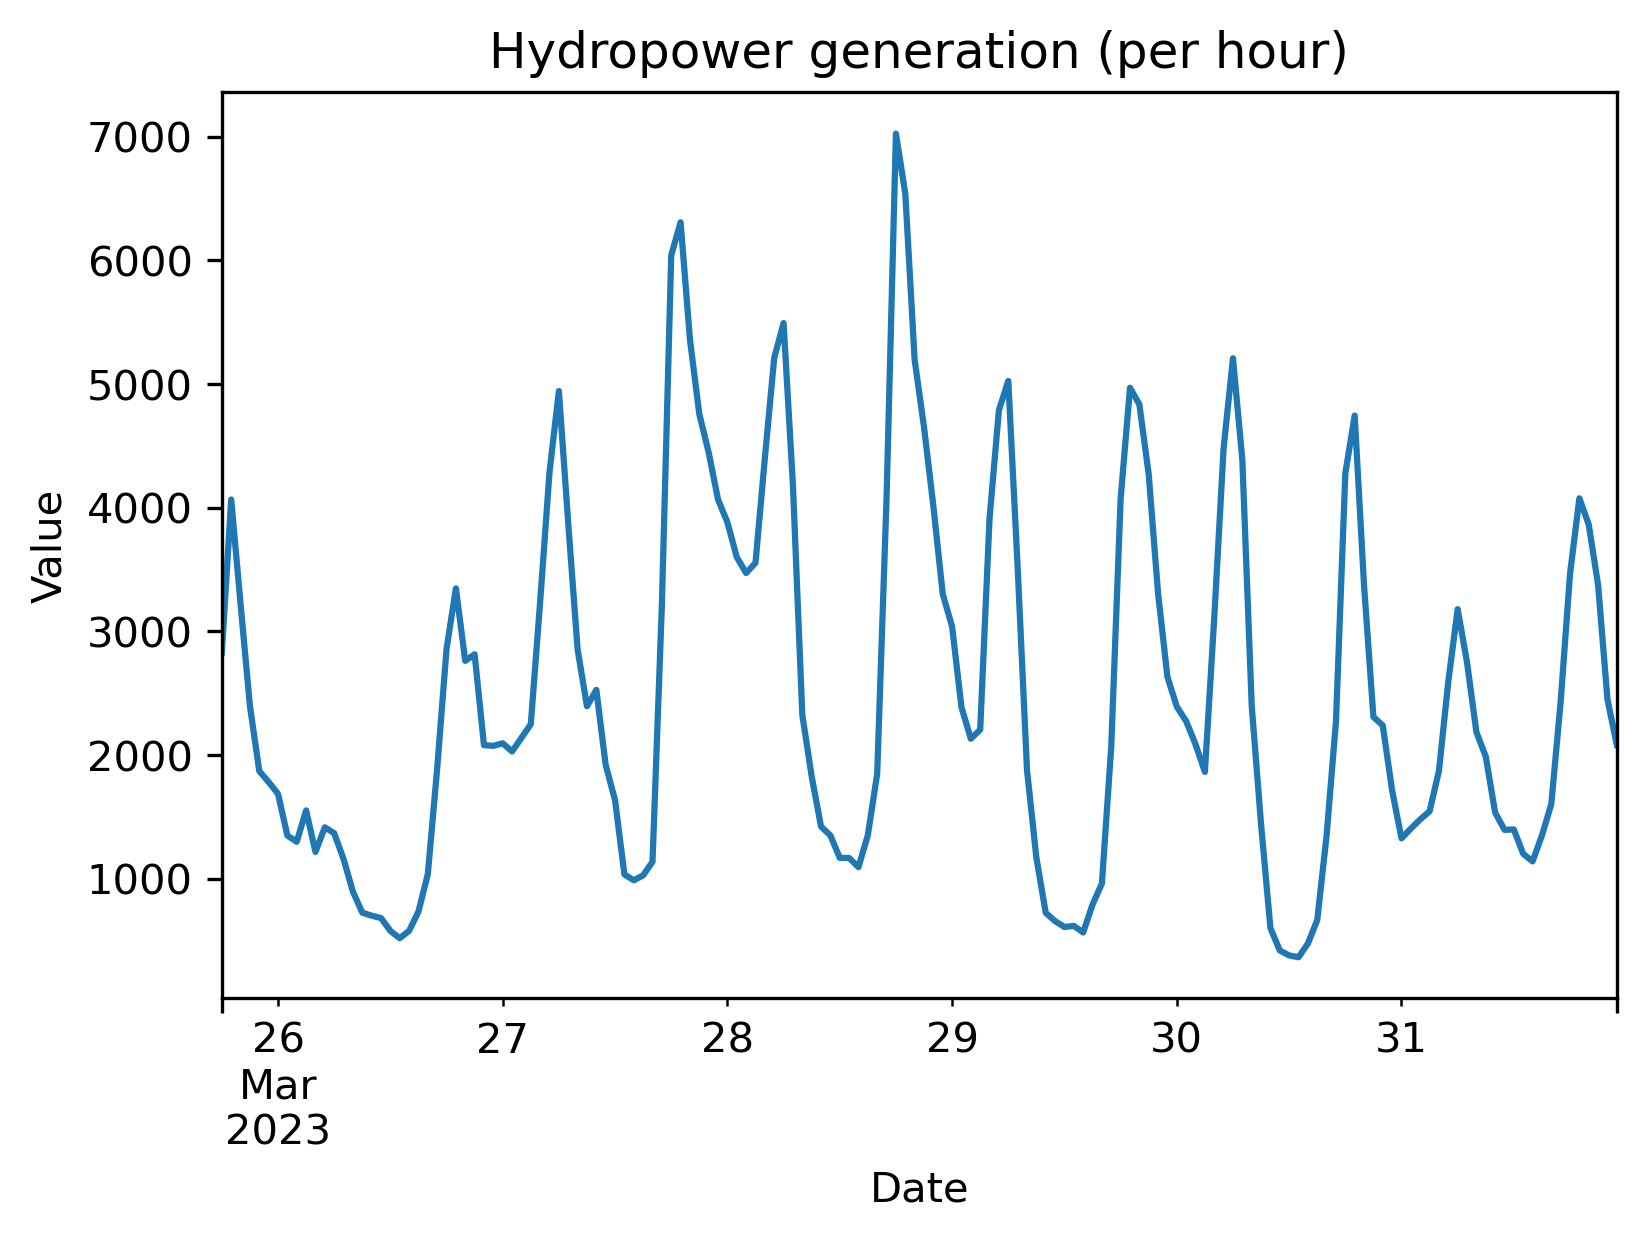
\includegraphics[width=1\linewidth]{images/variable_analysis/esios_generation_hydro_h_96}
        \caption{Hydropower per hour, 350 hours window.}
        \label{fig:hydro-series}
    \end{subfigure}
    \begin{subfigure}{.45\textwidth}
        \centering
        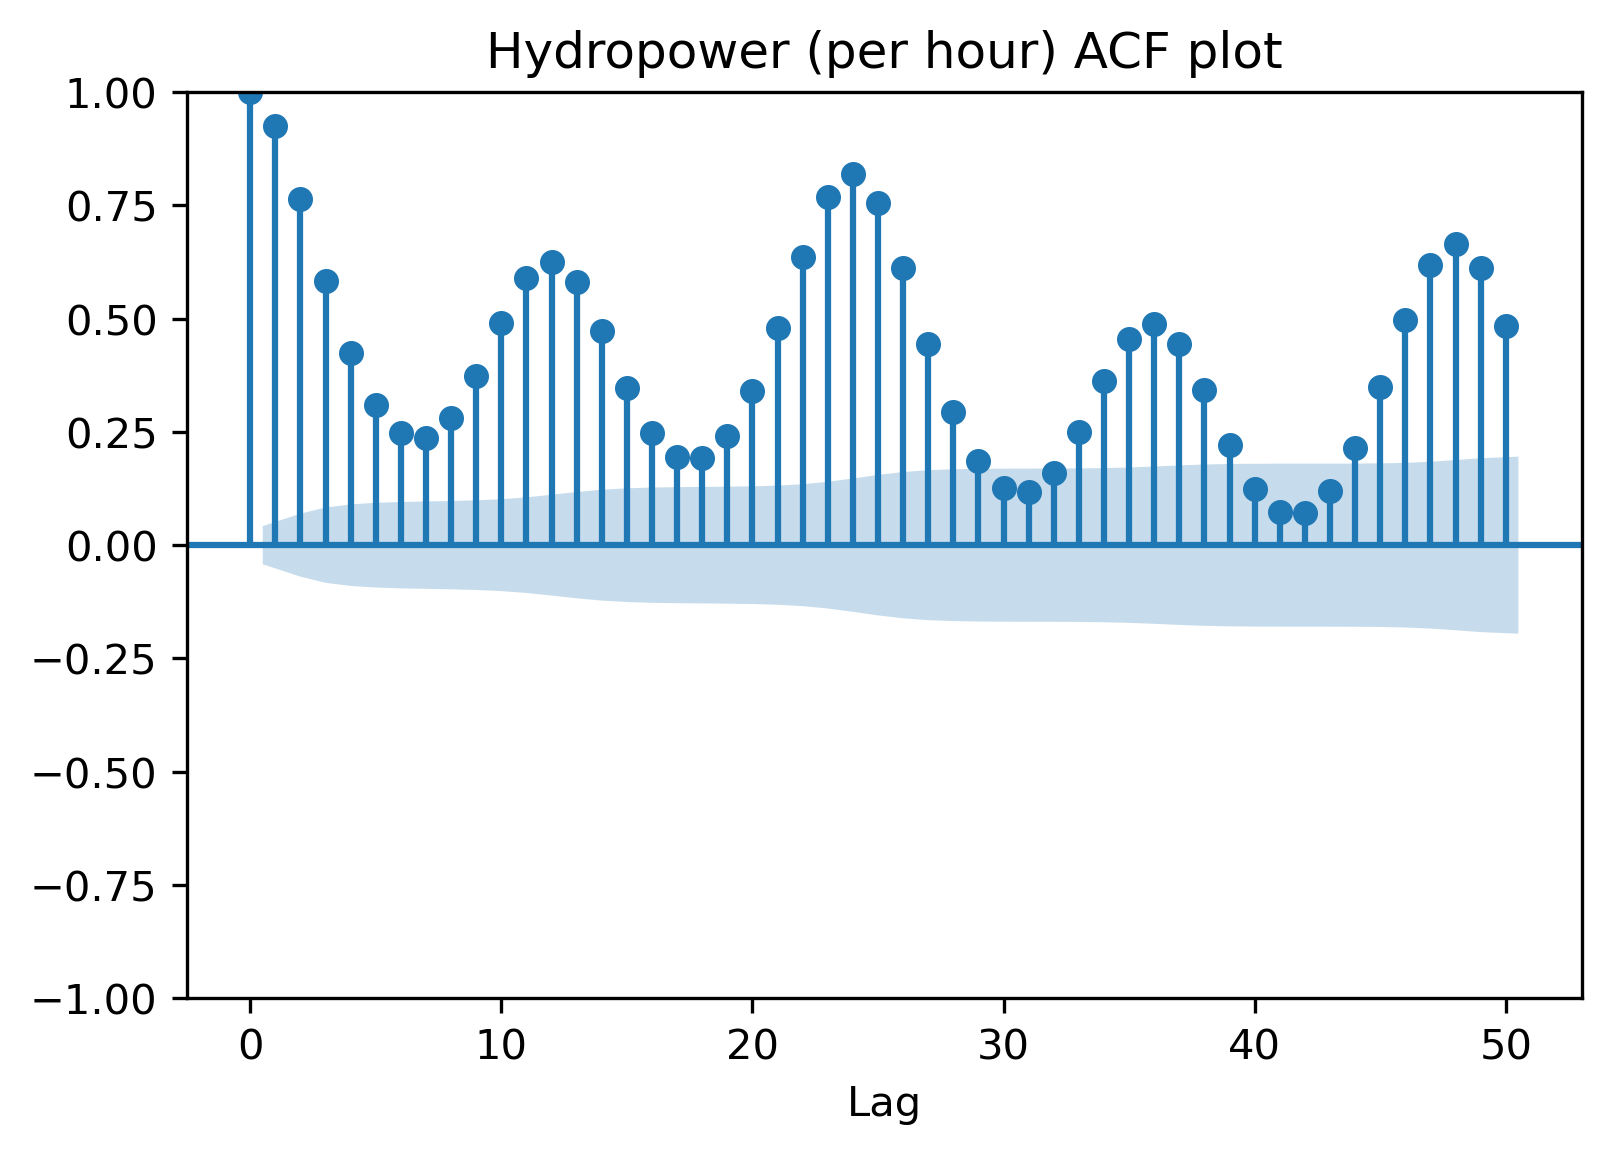
\includegraphics[width=1\linewidth]{images/variable_analysis/esios_generation_hydro_h_acf}
        \caption{Hydropower per hour, ACF plot.}
        \label{fig:hydro-acf}
    \end{subfigure}
\end{figure}

\begin{figure}[H]\ContinuedFloat
    \begin{subfigure}{.44\textwidth}
        \centering
        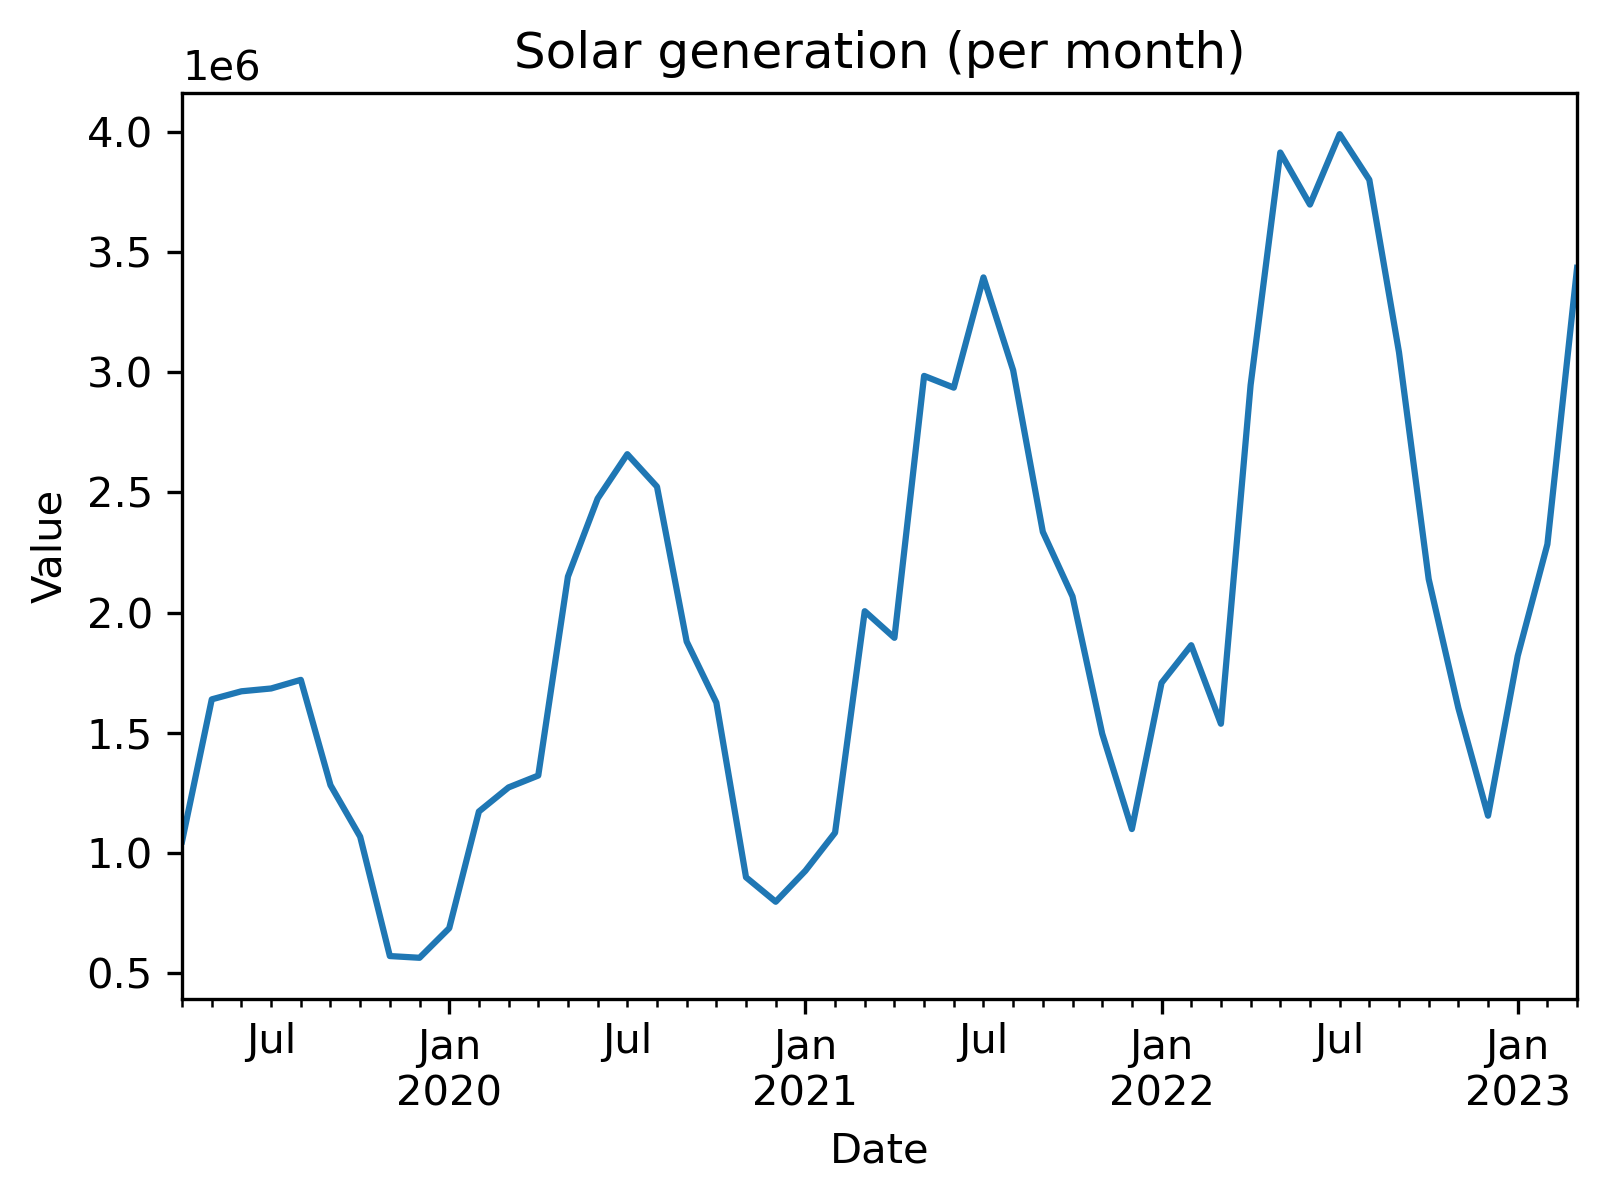
\includegraphics[width=1\linewidth]{images/variable_analysis/esios_generation_solar_m_48}
        \caption{Solar aggregated by day, 90 days window.}
        \label{fig:solar-series}
    \end{subfigure}
    \begin{subfigure}{.45\textwidth}
        \centering
        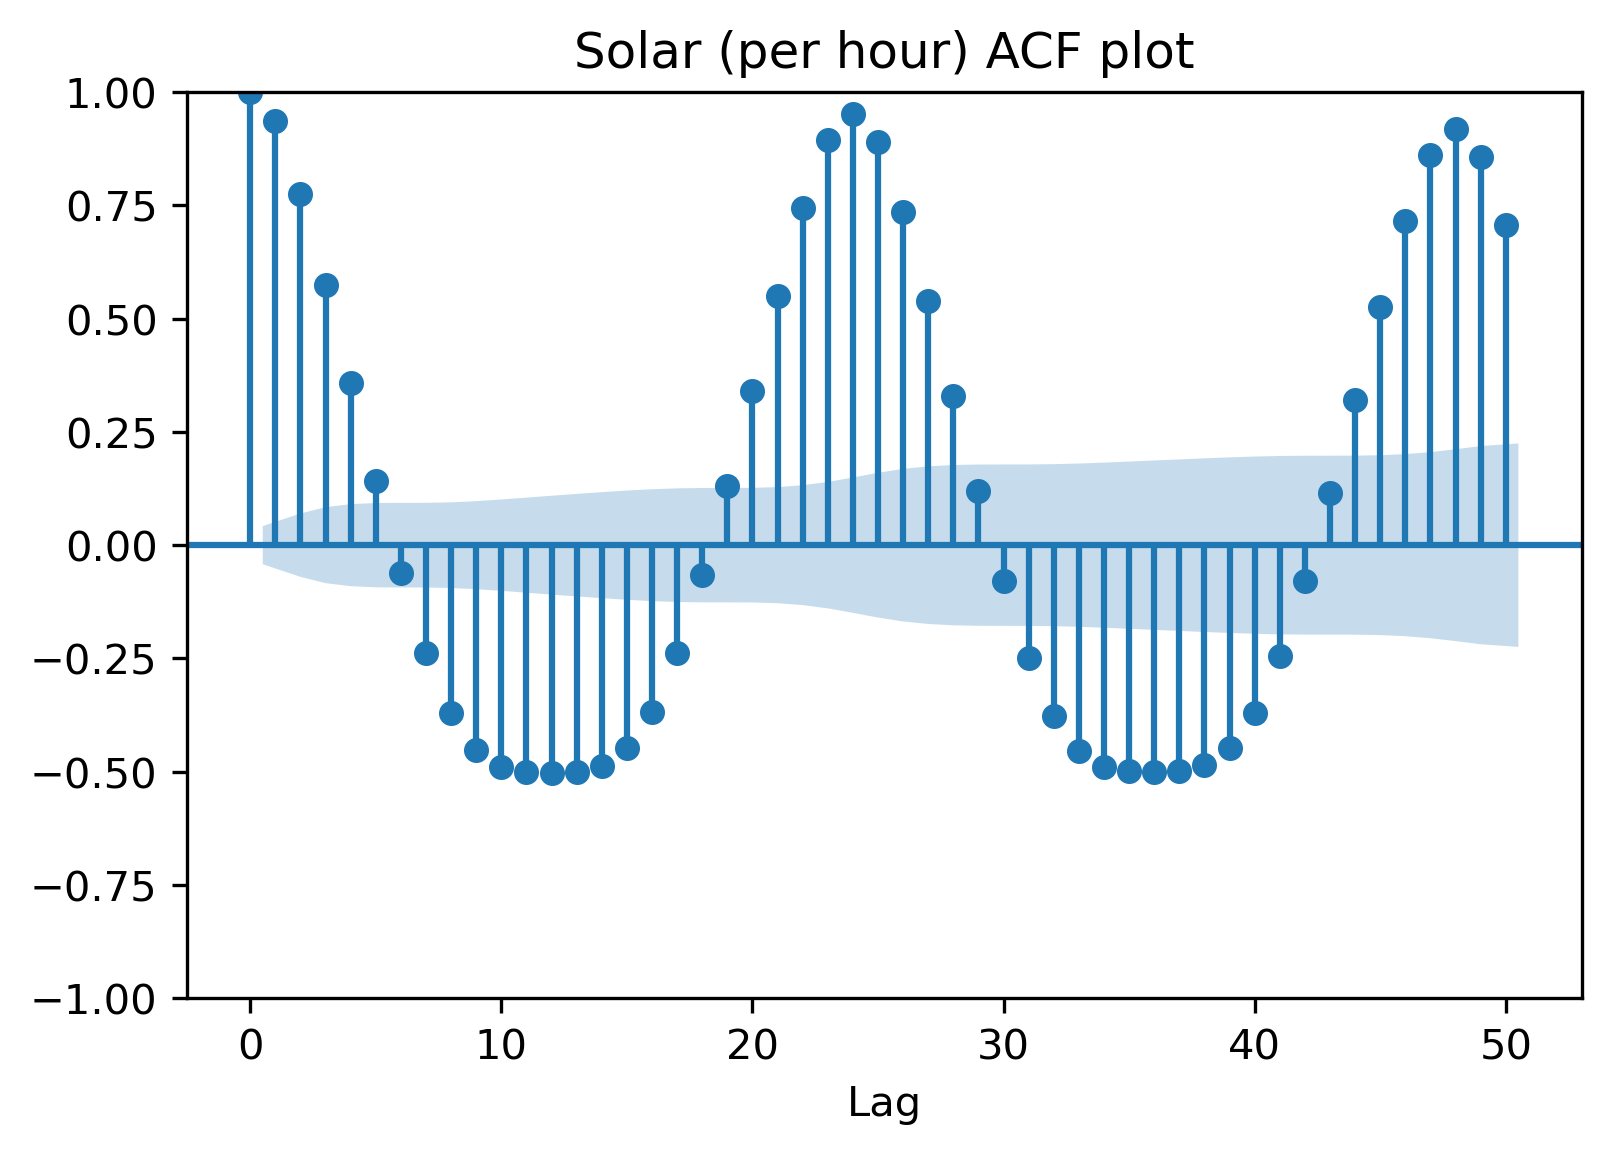
\includegraphics[width=1\linewidth]{images/variable_analysis/esios_generation_solar_h_acf}
        \caption{Solar per day, ACF plot.}
        \label{fig:solar-acf}
    \end{subfigure}
\end{figure}

\begin{figure}[H]\ContinuedFloat
    \begin{subfigure}{.43\textwidth}
        \centering
        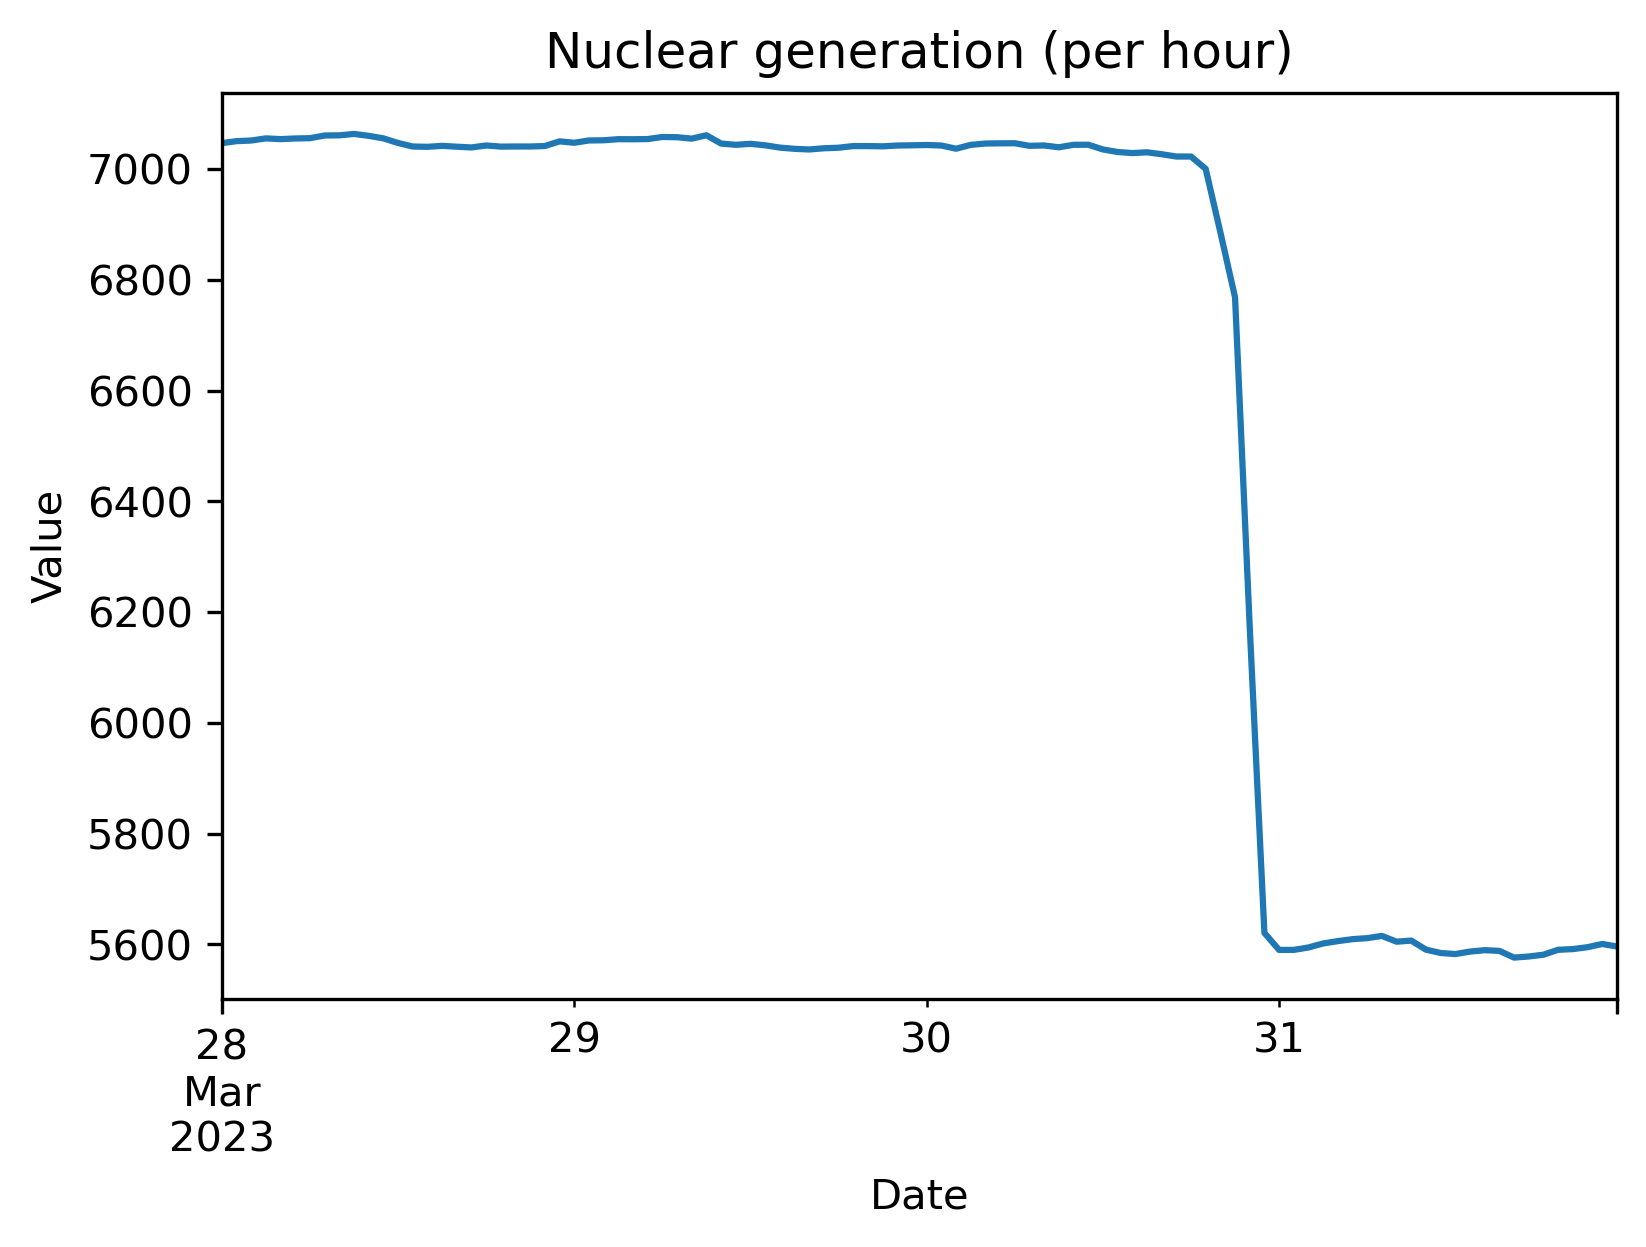
\includegraphics[width=1\linewidth]{images/variable_analysis/esios_generation_nuclear_h_96}
        \caption{Nuclear agg. by month, 40 months window.}
        \label{fig:nuclear-series}
    \end{subfigure}
    \begin{subfigure}{.47\textwidth}
        \centering
        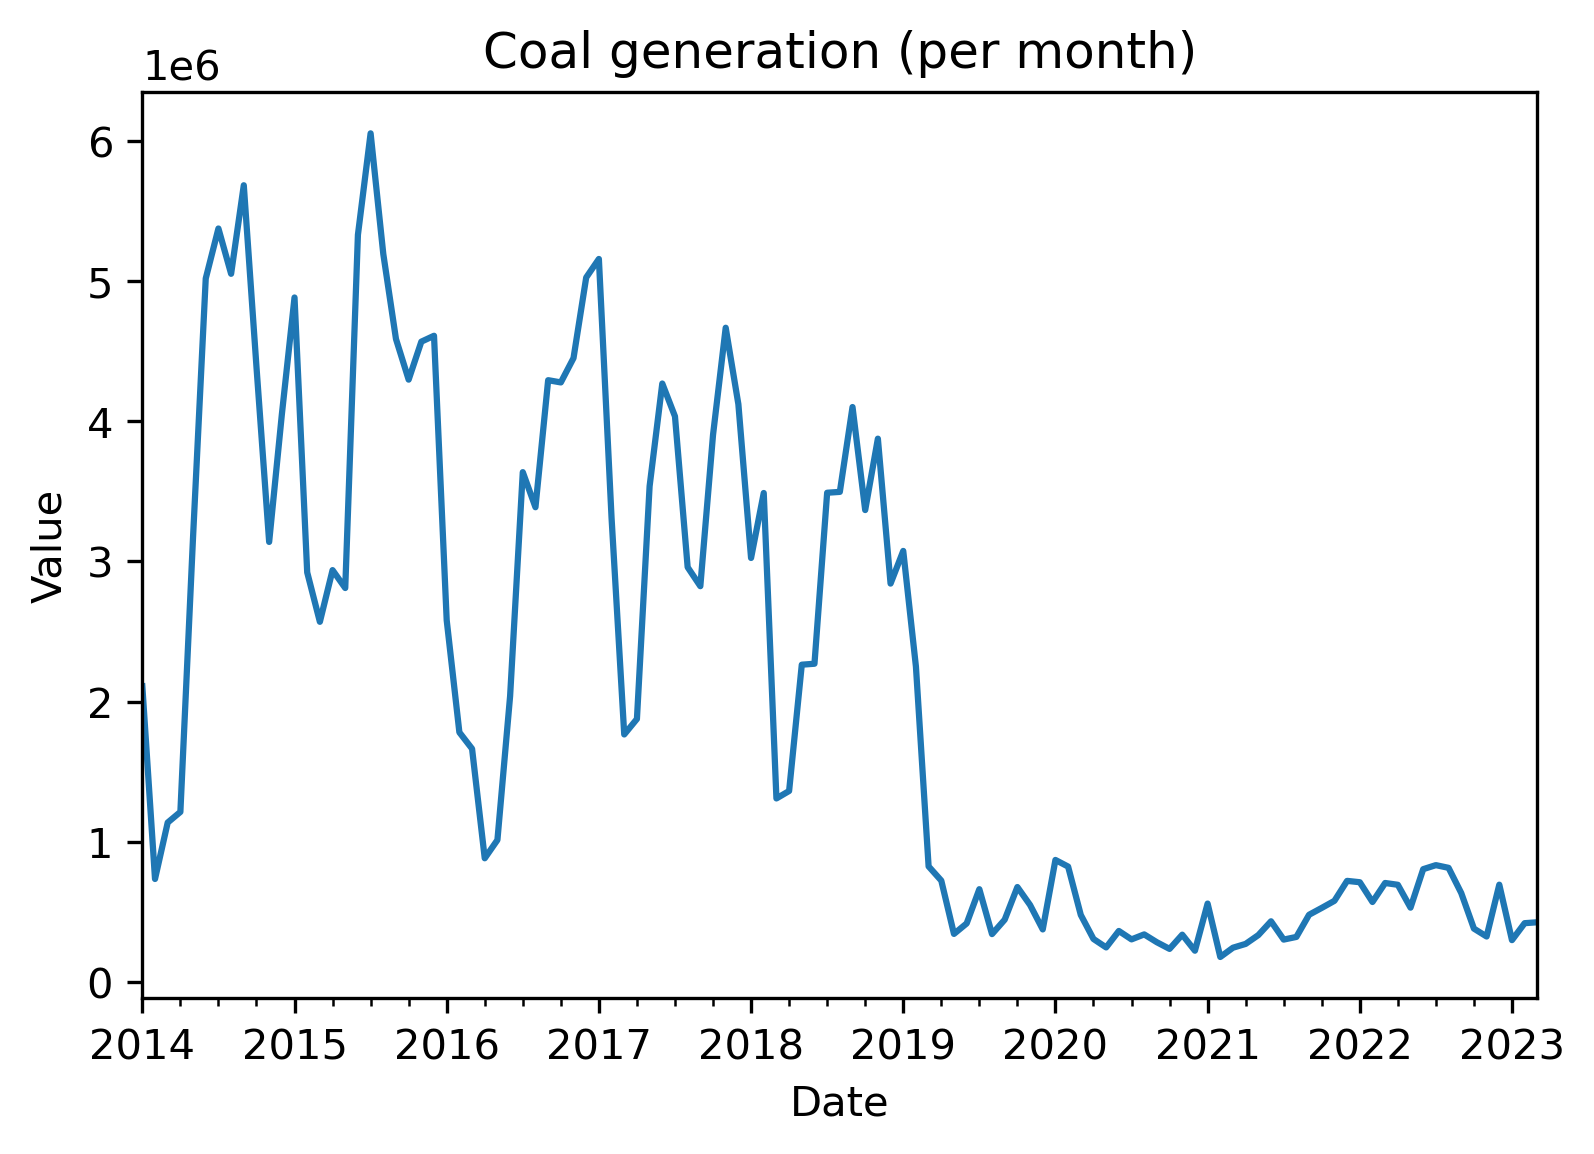
\includegraphics[width=1\linewidth]{images/variable_analysis/esios_generation_coal_m_all}
        \caption{Coal per month, complete series.}
        \label{fig:coal-series}
    \end{subfigure}

    \caption{Electricity demand curves analysis.}
    \label{fig:generation-series}
\end{figure}


\subsection{Price of commodities}
As the technologies using commodities to make energy usually set the market price, the price of these commodities could be also affecting it.
The author will study the influence of coal and gas.

Concretely, the gas prices in use will be the ones dictated by the TTF index, which have been downloaded from investing.com: from 10-2017 to 04-2023 in a daily fashion and from 04-2010 to 03-2023 in a yearly granularity. In the monthly case, the author works with the last observation in the month: that is because this is the only measure provided in the source, apart from minimum and maximum values in the period.

For the coal prices we will use the ARGUS/McCloskey index. Data has been downloaded from marketwatch.com, daily readings from 12-2010 to 03-2023.

As happened with electricity price, in Figure \ref{fig:commodities-series} we find a peak in prices in 2021 and 2022.

\begin{figure}[H]
\centering
    \begin{subfigure}{.45\textwidth}
        \centering
        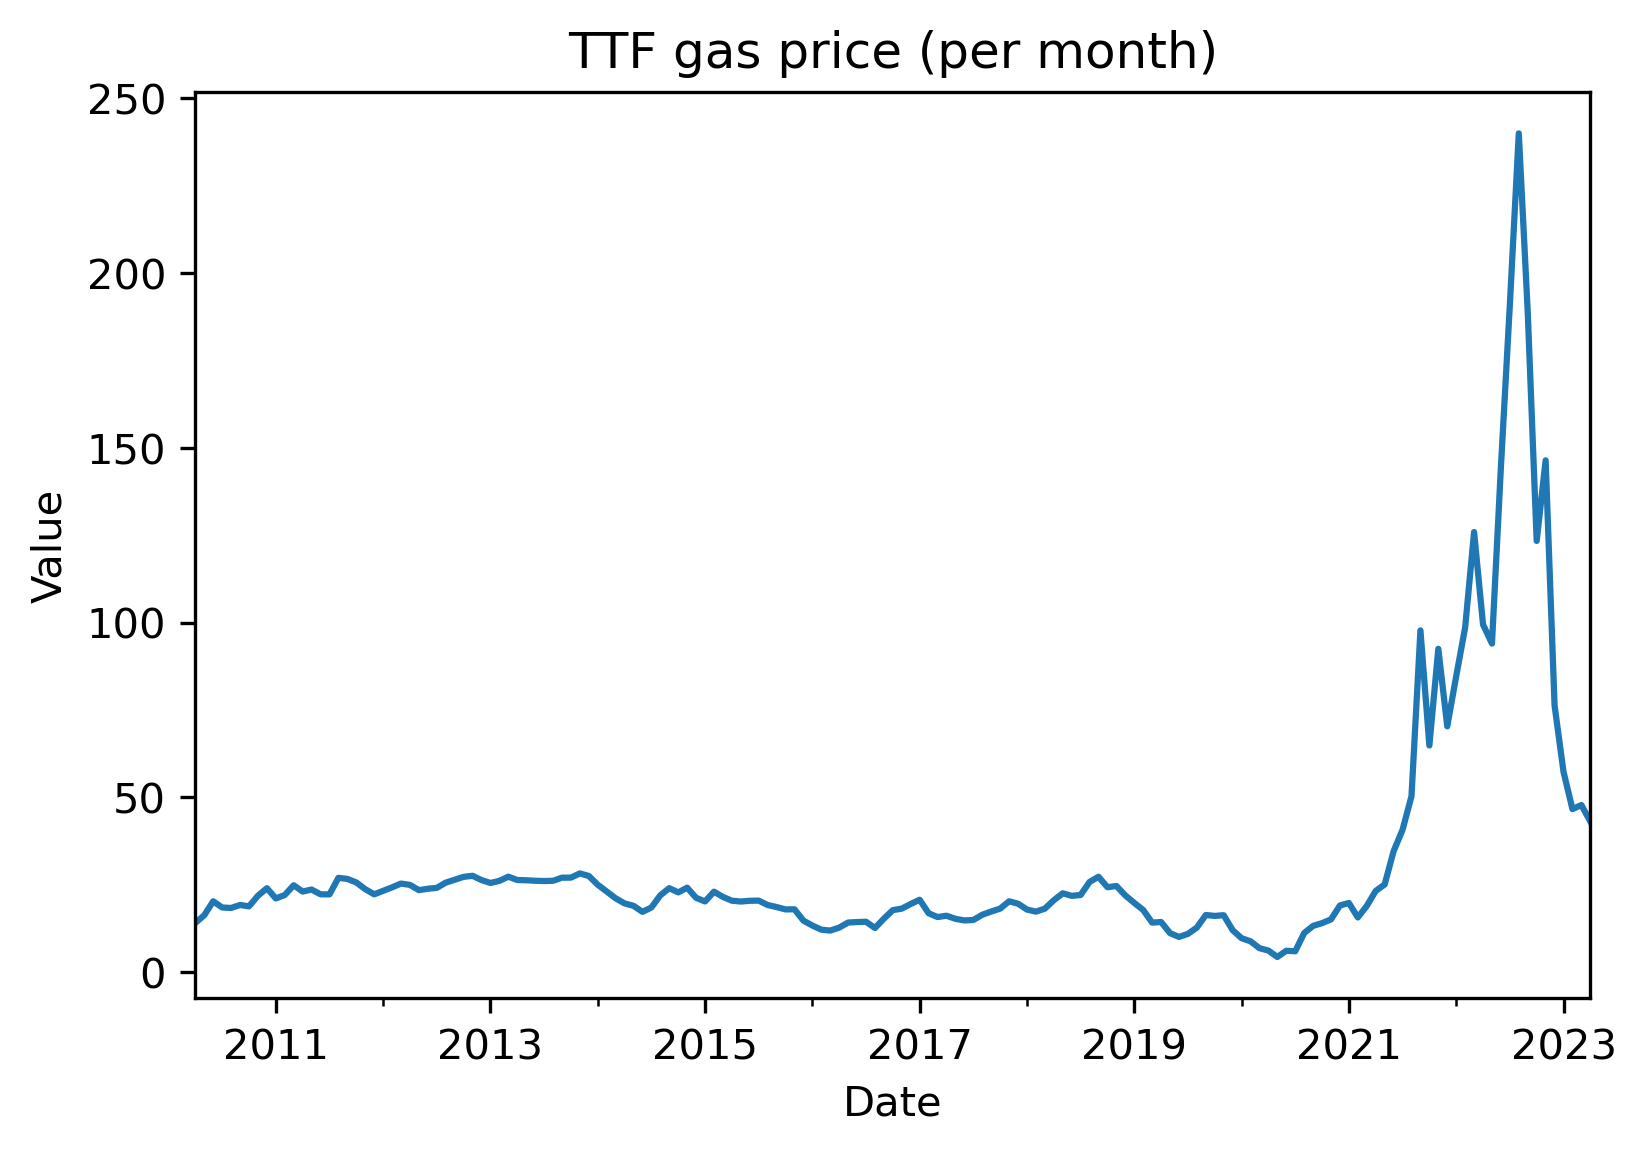
\includegraphics[width=1\linewidth]{images/variable_analysis/ttf_m_all}
        \caption{TTF gas price curve.}
    \end{subfigure}
    \begin{subfigure}{.45\textwidth}
        \centering
        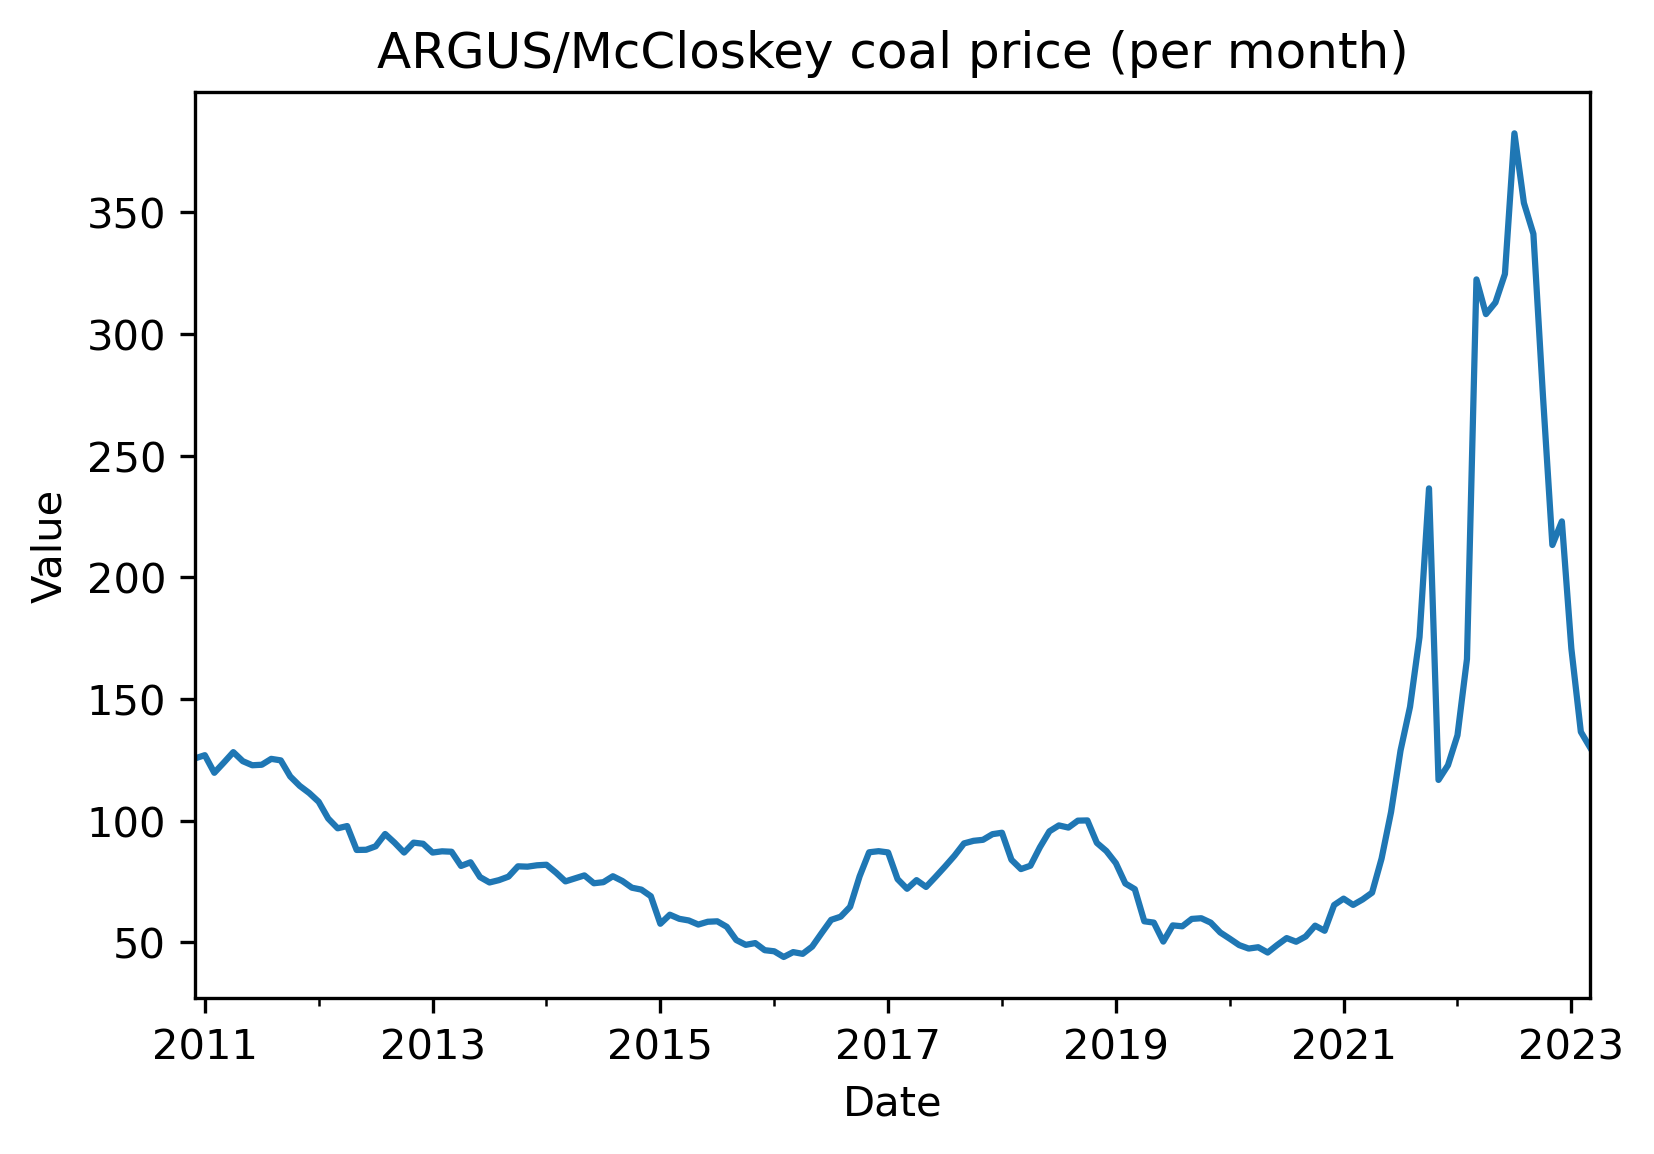
\includegraphics[width=1\linewidth]{images/variable_analysis/coal_m_all}
        \caption{ARGUS/McCloskey coal price curve.}
    \end{subfigure}

    \caption{Gas and coal price curves.}
    \label{fig:commodities-series}
\end{figure}

\subsection{EU Allowances (EUAs)}
The use of technologies producing carbon emissions requires to pay taxes to the European Union.
Companies buy allowances to be able to emmit $CO_2$ and they can trade with them, that's why allowances have market value which can influence the cost of energy.

The price of this allowance has been downloaded from International Carbon Action Partnership, having daily entries from 12-2010 to 03-2023. Monthly aggregated values are plotted in Figure \ref{fig:c02-euas-series}, we find an increase in its price in the previous years.

\subsection{Macroeconomic variables}
The economic situation affects prices in general, and therefore it can affect electricity cost.
GDP or inflation could be potential indicators to study. The author has chosen to study Spanish GDP downloading data from the World Bank, concretely from 1960 to 2021. We see an increasing trend for it in Figure \ref{fig:gdp-series}.

\begin{figure}[H]
\centering
    \begin{subfigure}{.45\textwidth}
        \centering
        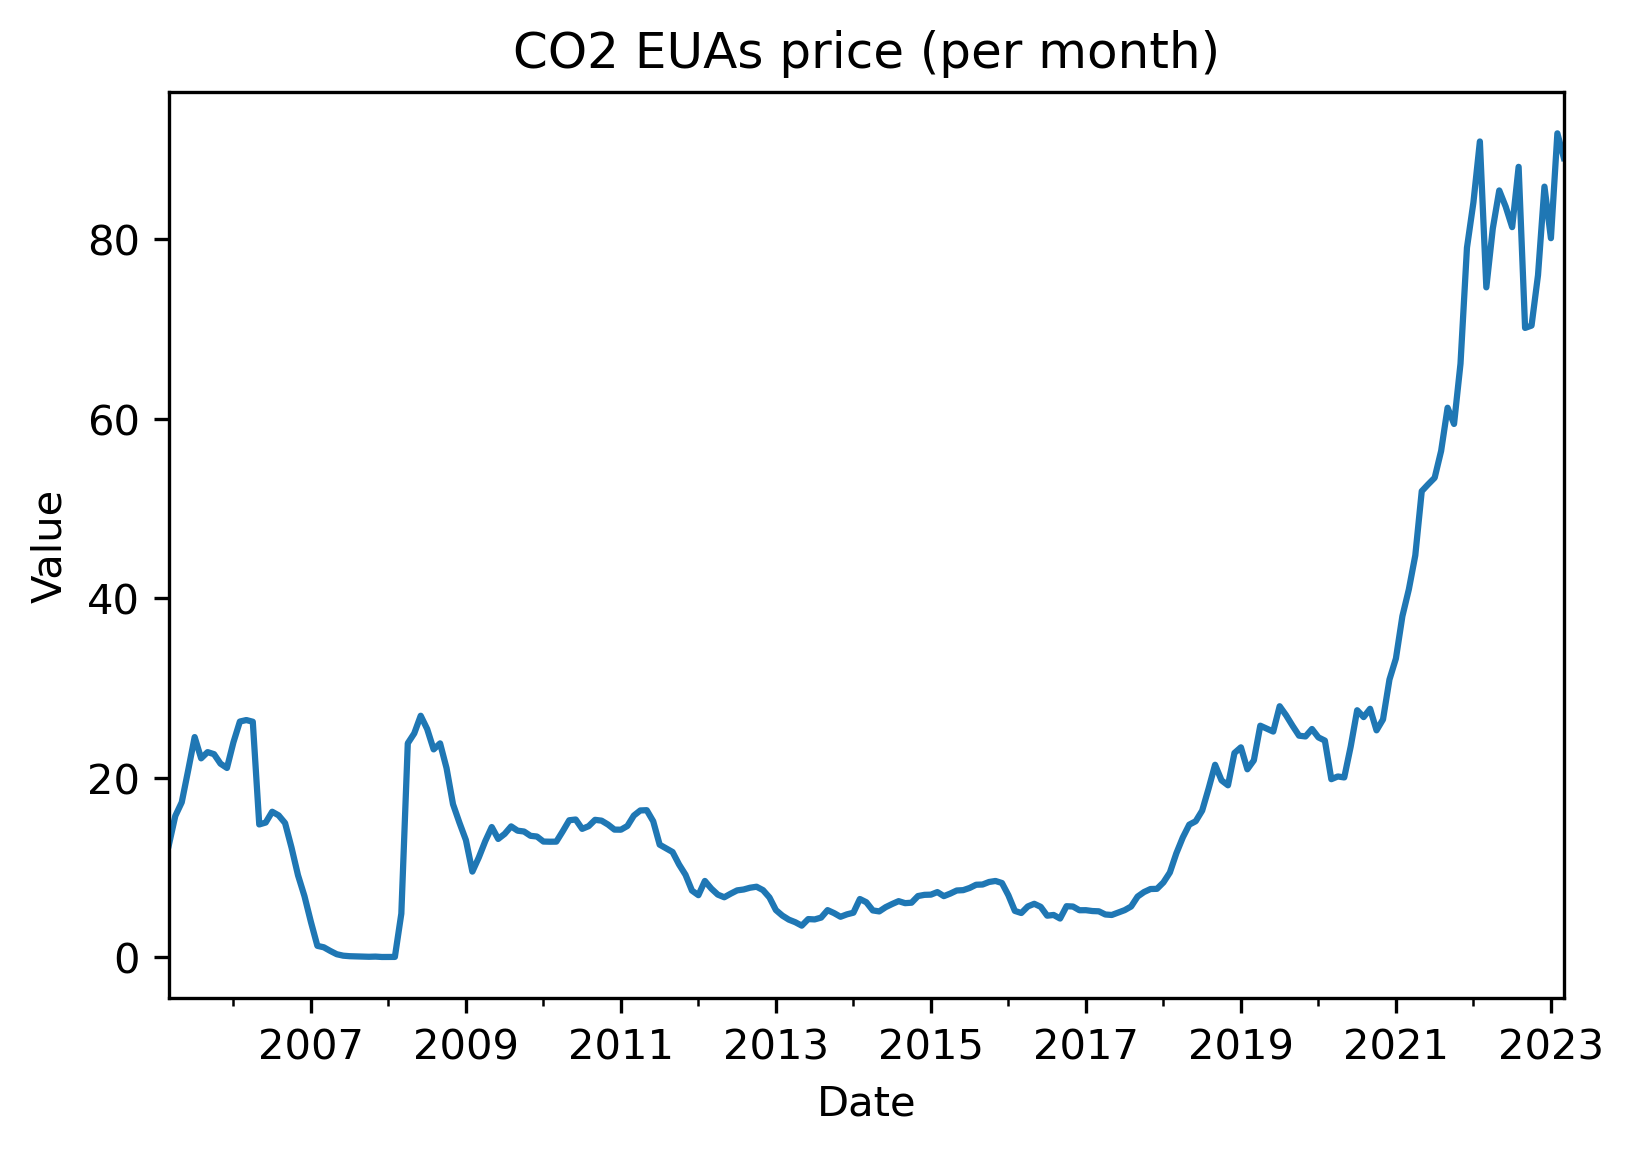
\includegraphics[width=1\linewidth]{images/variable_analysis/co2_m_all}
        \caption{CO2 European Allowances price.}
        \label{fig:c02-euas-series}
    \end{subfigure}
    \begin{subfigure}{.45\textwidth}
        \centering
        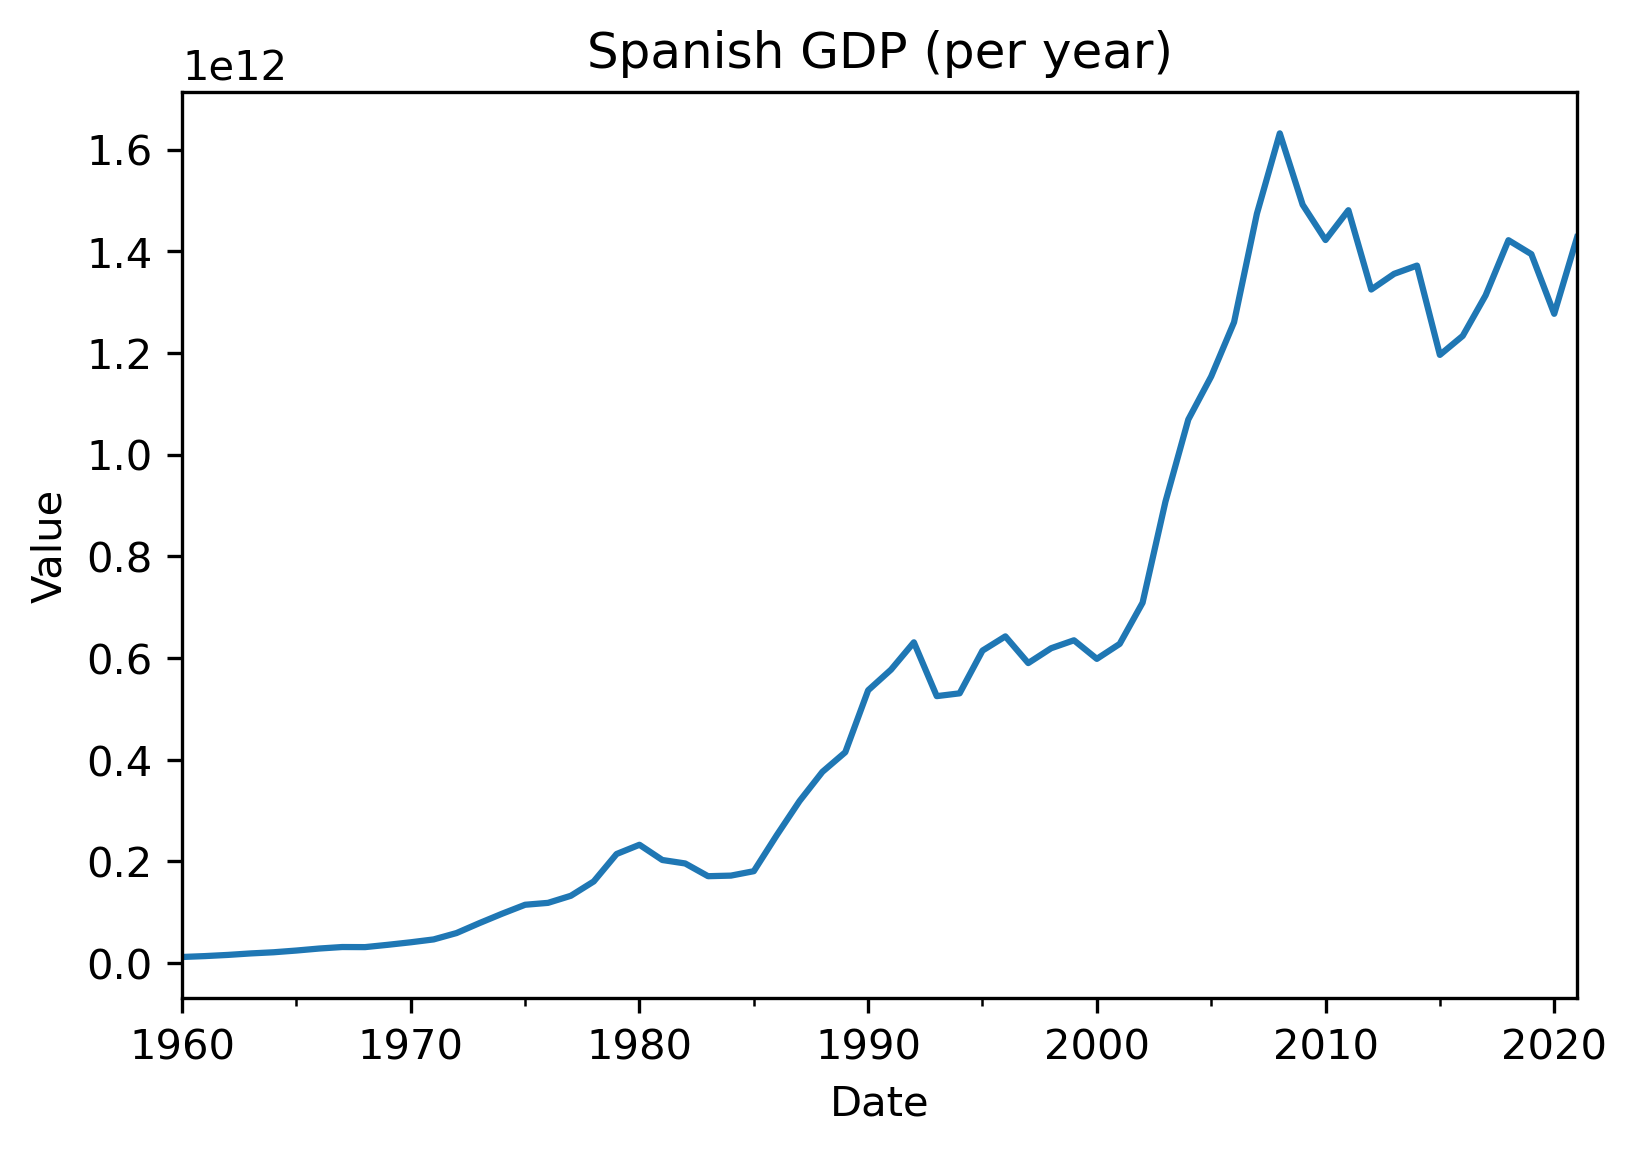
\includegraphics[width=1\linewidth]{images/variable_analysis/gdp_y_all}
        \caption{Spanish GDP.}
        \label{fig:gdp-series}
    \end{subfigure}

    \caption{CO2 EUAs and Spanish GDP series.}
    \label{fig:co2-gdp-analysis}
\end{figure}

\subsection{Time of day/week}
Something to consider is the moment for which the predictions are done.
The price is not the same during the day or night, or in weekdays or weekends.
This is correlated with the demand and the availability of renewable energy generation.

\vspace{1.3cm}

The previous predictors can improve the model capabilities, as they could add extra explicative information about the price.
In the next sections the author will analyze which of them are explaining the most in the specific studied models.


\chapter{Research methodology and implementation}
\label{ch:methodology}
In this chapter the author is designing the methodology to be followed in the experiments. This is an important step, as building it correctly will lead to significant and meaningful results.
We discuss three phases: data acquisition and preprocessing, price forecasting and predictor's importance.

In the first phase, all the necessary data will be downloaded with the finest possible granularity.
When studying broader timespans, it will be aggregated.

In the last two phases the author explains the design of the experiments: the same procedure will be used to analyze in an hourly, daily and monthly fashion, changing the parameters for every case.
On the other hand, for the yearly level, as there is not enough data to perform an statistical study, a descriptive and visual analysis will be performed.

\section{Data acquisition and preprocessing}
TODO

\subsection{ML models need tabular form}
In classical time series models as ARIMA, data can be directly introduced in the model without restructuring it.
But when we use ML-based architectures, data has to be reshaped so the models can recover autocorrelation.
This is why the author arranges it in the tabular form described in Figure \ref{fig:ml-arrangement}.
On it, the response (price) and predictors (as could be demand or generation) are included together with some response lags.

\begin{figure}[H]
\centering
    \caption{Tabular form in which data is disposed for ML models. On it, n is the number of observations in the time series and k is the number of lags in use.}
    \label{fig:ml-arrangement}
    \fbox{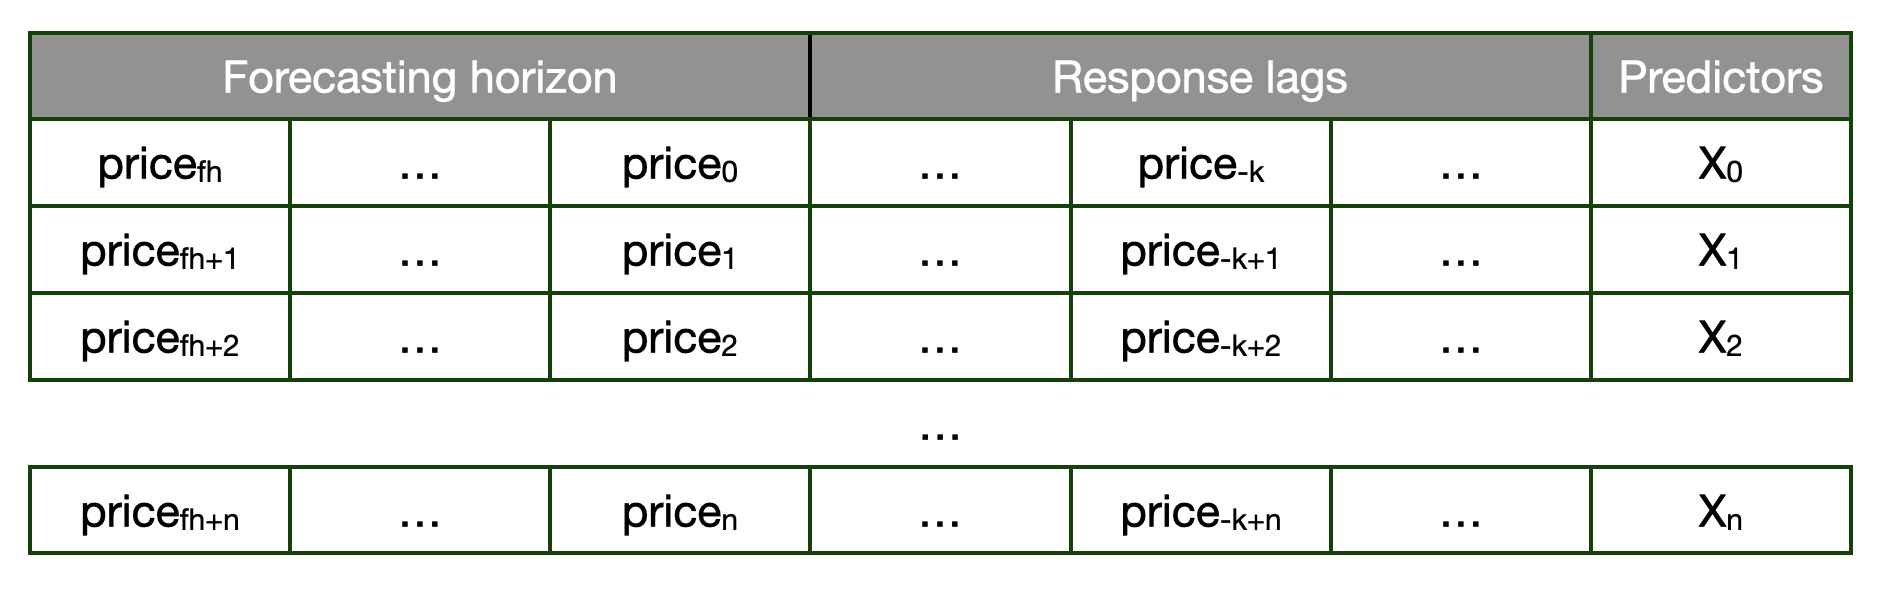
\includegraphics[scale=0.4]{images/methodology/ml_arrangement}}
\end{figure}

The author has decided to implement this table generation manually, to exactly control the lags to use on each case.

\section{Price forecasting}
The library used to perform forecasts is \textit{sktime} \cite{DBLP:journals/corr/abs-1909-07872}: it simplifies the implementation, reducing boilerplate code and making the scripts cleaner.

\subsection{ML models to compare}
We will test different models, analyzing which of them work better:
\begin{itemize}
    \item k-Nearest Neighbors (kNN)
    \item Random Forest (RF)
    \item Gradient Boosted Trees (GBT)
    \item Support Vector Machine (SVM)
    \item Dummy regressor (DR), acting as baseline.
\end{itemize}
All of them are implemented in \textit{scikit-learn} and integrated in \textit{sktime} by the use of \textit{make\_reduction()} function. On it, the parameter \text{strategy} needs to be specified: there are two possible strategies to forecast each value in the forecasting horizon, direct and recursive.

The former creates one model for each value in the forecasting horizon, the latter applies a recursive process in which each new prediction is based on the previous one \cite{direct-recursive-forecasting}, so only one model is created. See Figure \ref{fig:direct-recursive-forecasting}. Direct strategy is what is used on this project, as it is more precise. On the other hand, it is computationally expensive.

\begin{figure}[H]
\centering
    \begin{subfigure}{.45\textwidth}
        \centering
        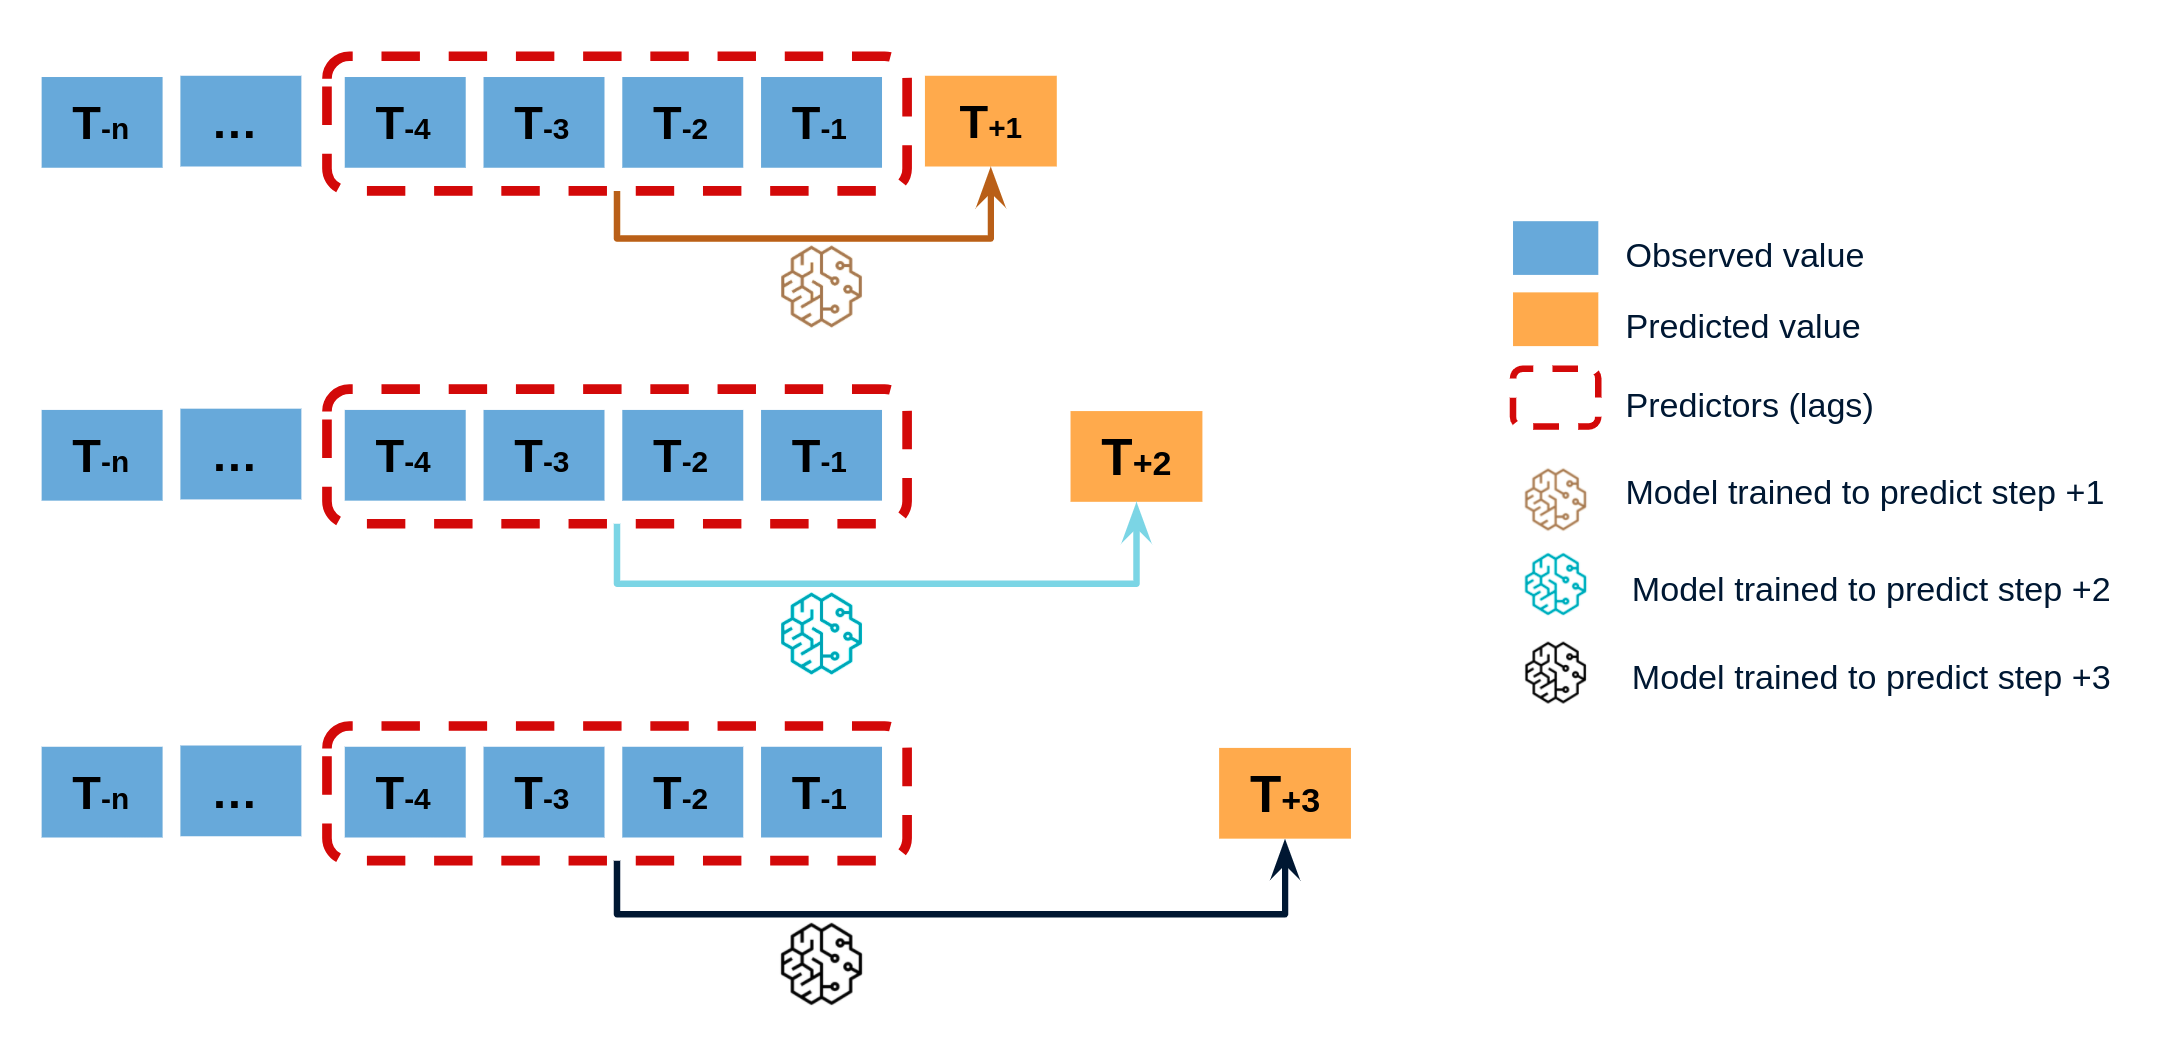
\includegraphics[width=1\linewidth]{images/methodology/direct-multi-step-forecasting}
        \caption{Direct forecasting.}
    \end{subfigure}
    \begin{subfigure}{.45\textwidth}
        \centering
        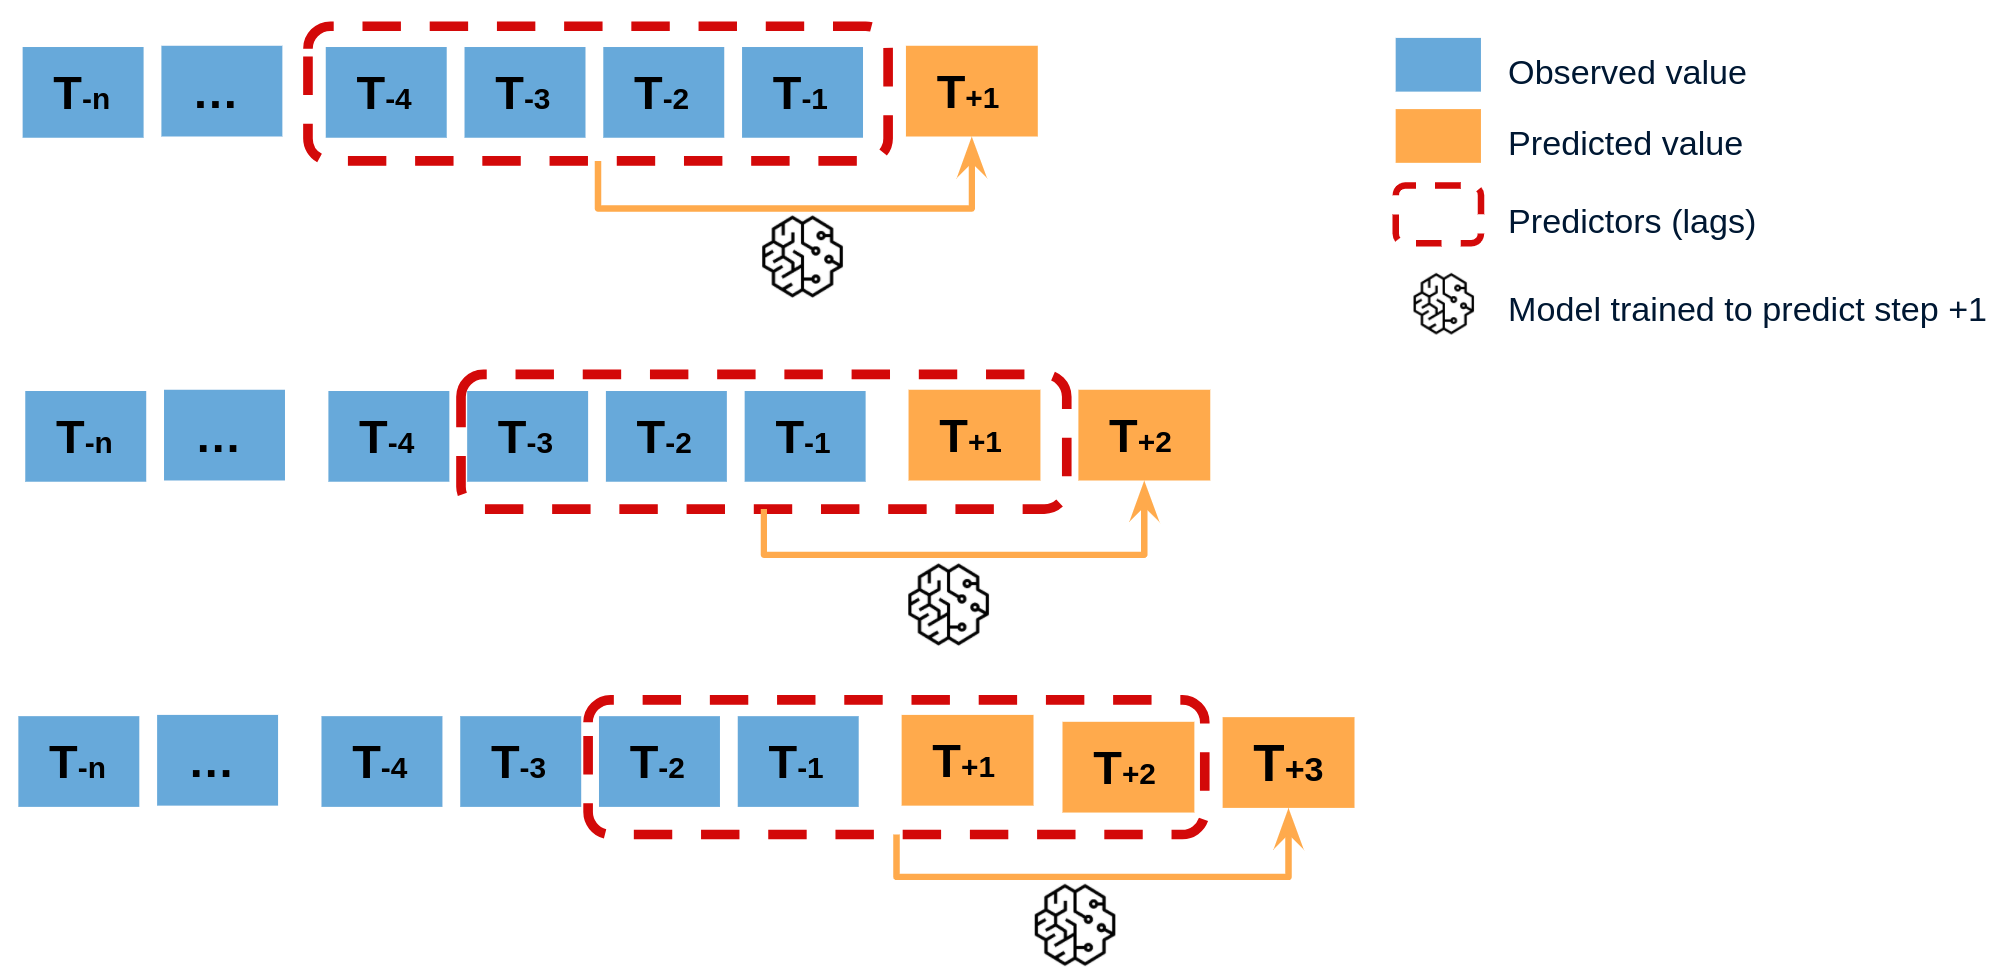
\includegraphics[width=1\linewidth]{images/methodology/recursive-mutistep-forecasting}
        \caption{Recursive forecasting.}
    \end{subfigure}

    \caption{Direct vs recursive forecasting strategies.}
    \label{fig:direct-recursive-forecasting}
\end{figure}

\subsection{Compare ARIMA with ML models}
All the previously mentioned models are ML based. Some as those based on tree ensembles are very powerful, but they come with some drawbacks compared with their purely based on statistics counterparts. For instance, they need more data to be trained.

This is why on the medium and long term forecasts, as we have less datapoints, we are also testing the performance of ARIMA models so we get an idea of how non-ML models can perform in this situation.

In ARIMA (and generally in classical TS models) it is important to treat the window size as an hyperparameter. The performance of these models can change depending on how many datapoints we use to train.

\subsection{Loss function}
To compare the performance between different models, the author will use the Mean Absolute Scaled Error (MASE) loss function described in Equation \ref{eq:mase}:
\begin{equation}
    \label{eq:mase}
    \mathrm{MASE} = \frac{1}{N}\sum_{k=1}^{N}\frac{|p_k-\hat{p}_k|}{\frac{1}{n-1}\sum_{i=2}^{n} |p^\mathrm{in}_i - p^\mathrm{in}_{i-1} |},
\end{equation}

\subsection{Performance evaluation}
This process will be performed in two steps. In the first, we compare the performance of the different models using cross validation. Once we know which returns the higher score, we train it over all the cross-validation data and give a final estimation over a test set. See Figure \ref{fig:cross-train-test}.

\begin{figure}[H]
\centering
    \caption{Data splitting to peform model selection and final model performance estimation.}
    \label{fig:cross-train-test}
    \fbox{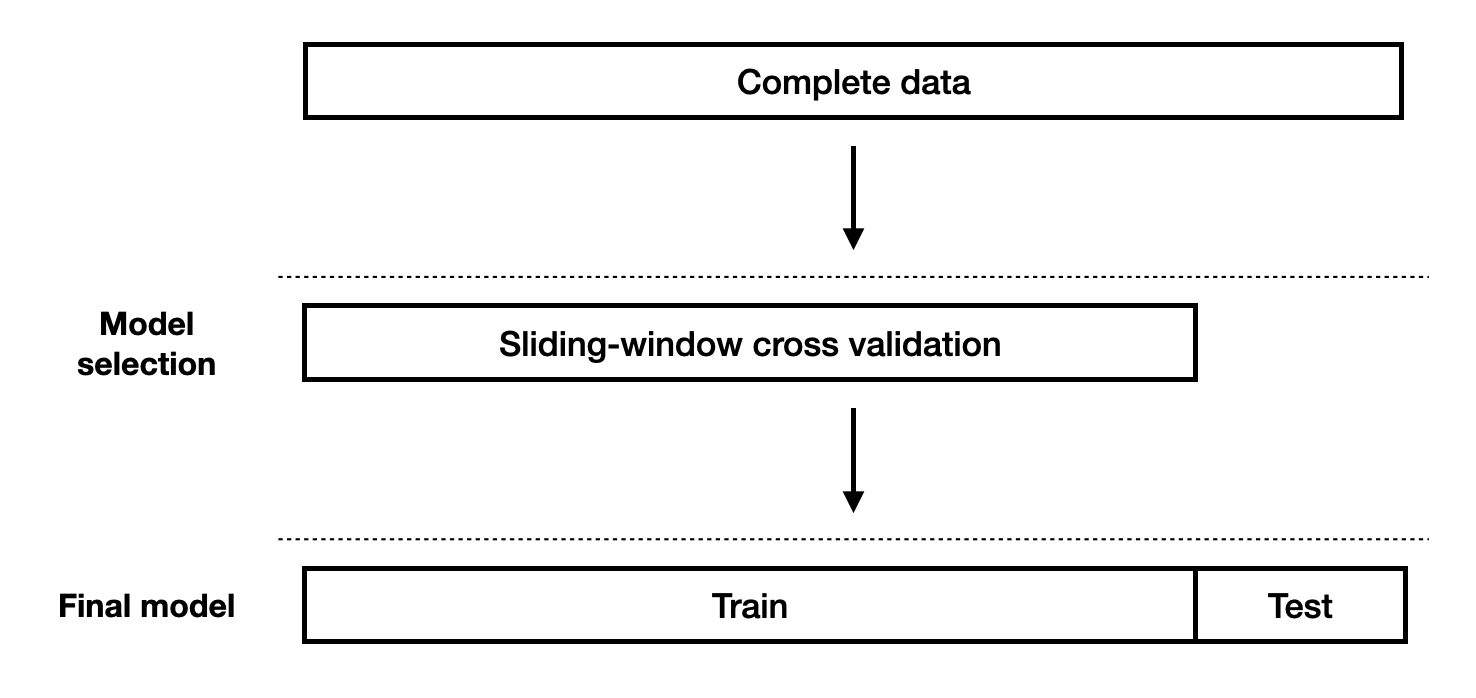
\includegraphics[scale=0.4]{images/methodology/cross_train_test}}
\end{figure}

\subsubsection{Model selection}
Two well known strategies used to divide data to perform model selection are holdout and cross-validation.
In the former, data is partitioned in two splits, train and test, e.g. 80\% train and 20\% test.
The problem with this strategy is that we are only assessing the performance of the model in a reduced portion of data.
On the other hand, if we use cross-validation we divide the data in multiple folds: on an iterative process, one is reserved for testing and the rest for training, changing the test fold on every iteration.
At the end, we manage to assess the performance in the complete dataset.

\noindent But using k-fold cross validation is not suitable for time series forecasting \cite{cross-validation-types}:
\begin{enumerate}
    \item Test data can appear before train data.
    \item Data leakage can happen if test data appears after train folds, as the model knows extra information about the future.
\end{enumerate}

There exist other techniques that solve this problem, for example sliding or expanding window cross validation.
In sliding window splitters, the folds are created by scrolling a window of constant size through data.
This window is divided into train and test, maintaining the size of both partitions on all the windows.

In the case of expanding windows, its size is not constant but it grows. Concretely, the test partition remains the same through different windows and the train one grows collecting all the previous observations.

In Figure \ref{fig:sliding-expanding-windows} the author exposes a comparison between both strategies. For this project we are using sliding windows.

\begin{figure}[H]
\centering
    \caption{Sliding vs expanding windows \cite{sliding-expanding-windows}.}
    \label{fig:sliding-expanding-windows}
    \fbox{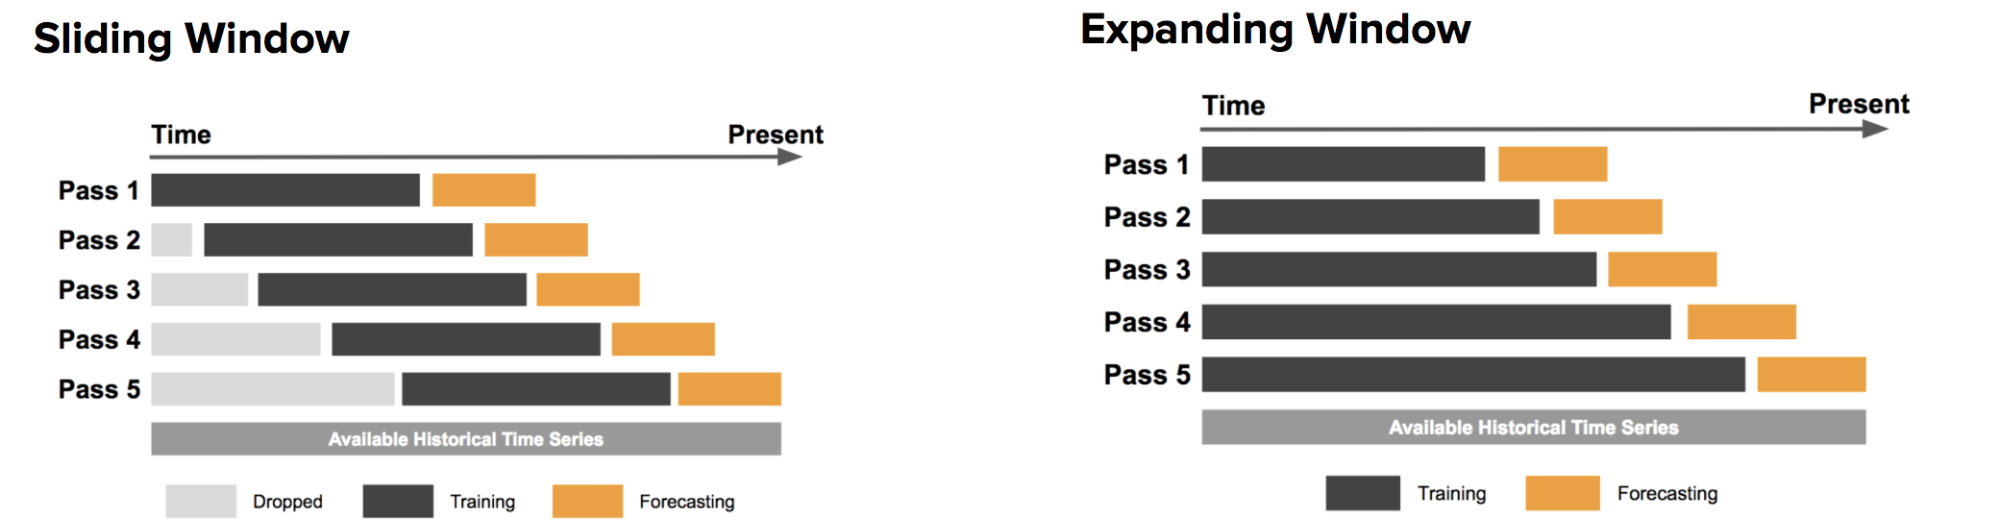
\includegraphics[scale=0.2]{images/methodology/sliding-expanding-windows}}
\end{figure}

Once that the data has been preprocessed and the cross-validation pipeline has been built, is time to run it.
The results will indicate which is the most suitable model on each case.

\subsubsection{Best model forecast}
Now that the most suitable model is known, it is trained over the data used for cross validation and tested  over new data that haven't been used previously.
That data corresponds to the newest values in the series.

This will be the final prediction shown in this report, together with a final performance estimation.

\section{Predictor's importance with SHAP values}
As we studied in Chapter \ref{ch:state-of-the-art}, SHAP values are a state-of-the-art way of explaining predictor's importance in ML models. Unluckily, the existing implementations are not compatible with \textit{sktime}. On the other hand, the implementation in \cite{shap-package} works with \textit{scikit-learn} models.

To study which variables affect the electricity price, a different strategy to what is done in forecasting is followed. Instead of training a model for each point in the forecasting horizon, we only create for the first and last values. Over the results of this two models we will apply the SHAP computation.

The study is performed in this way because interpreting SHAP values for each individual forecast horizon point is not viable. Another option would be to average the SHAP values for all the points, but the author thinks that this will make the results less interpretable.

The architecture used for the two models is the one that returned the best result in forecasting. They work over tabular data disposed like in Figure \ref{fig:shap-arrangement}. Once tabulated, data is divided into train and test (Figure \ref{fig:shap-train-test}): the train split is used to train the models and the test partition is the one over the SHAP value are computed.

Nevertheless, there is one exception: if the best performing model is ARIMA, the SHAP values are computed over the best ML model, not over ARIMA. This is because the SHAP package is not directly compatible with ARIMA implementation.

\begin{figure}[H]
\centering
    \begin{subfigure}{.95\textwidth}
        \centering
        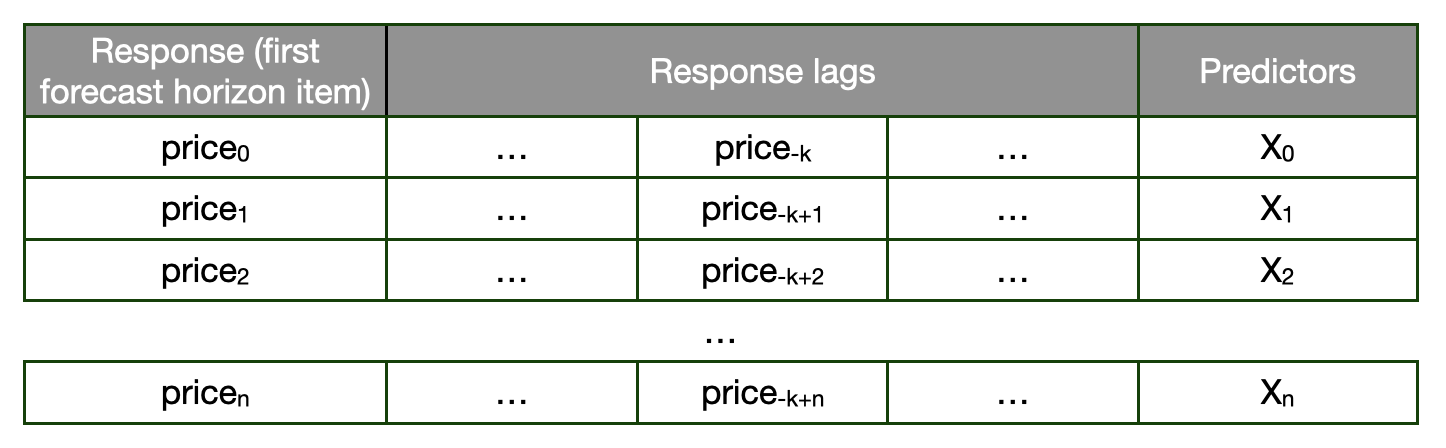
\includegraphics[width=1\linewidth]{images/methodology/shap_arrangement_first}
        \caption{Disposition for the first value case in the forecasting horizon.}
        \label{fig:shap-arrangement-first}
    \end{subfigure}
    \vspace{0.3cm}
    \begin{subfigure}{.95\textwidth}
        \centering
        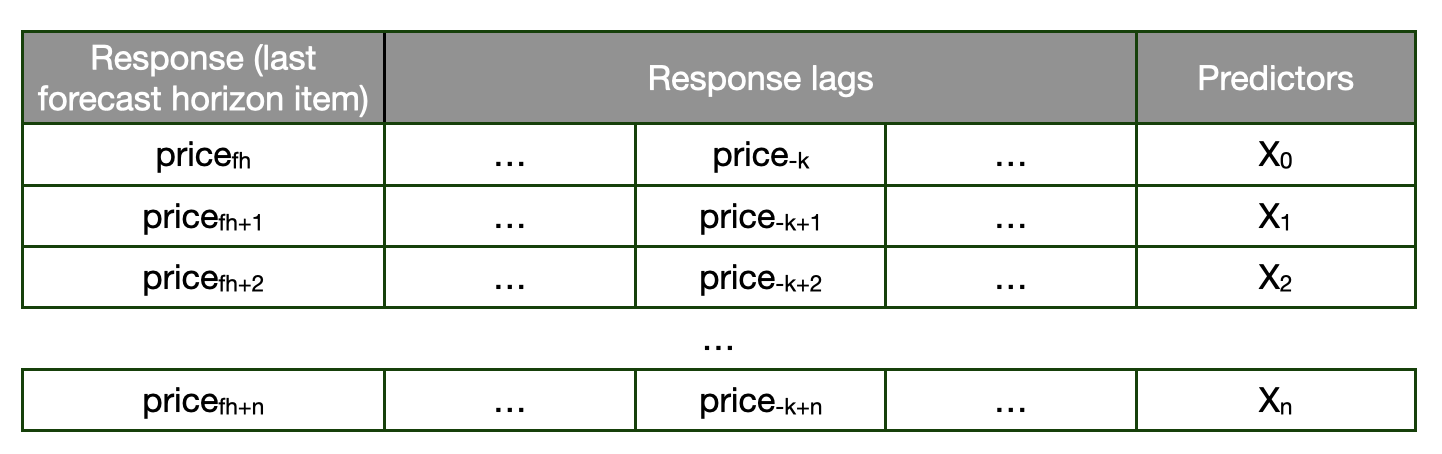
\includegraphics[width=1\linewidth]{images/methodology/shap_arrangement_last}
        \caption{Disposition for the last value case in the forecasting horizon.}
        \label{fig:shap-arrangement-last}
    \end{subfigure}

    \caption{Data disposition to evaluate the influence of predictors.}
    \label{fig:shap-arrangement}
\end{figure}

\begin{figure}[H]
\centering
    \caption{Train/test split of the tabular data used to compute the SHAP values.}
    \label{fig:shap-train-test}
    \fbox{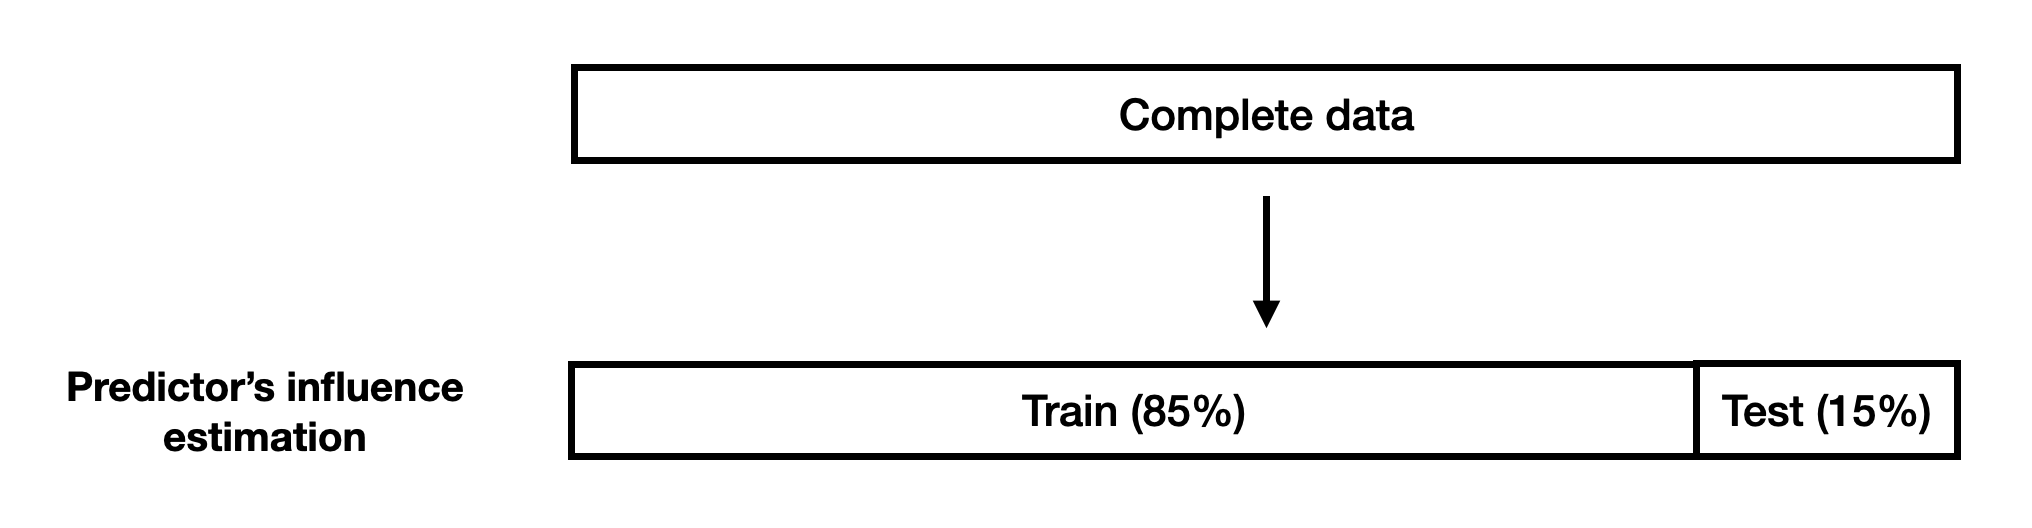
\includegraphics[scale=0.38]{images/methodology/shap_train_test}}
\end{figure}


%\section{Yearly forecasting}
%Judgmental forecasting
%\chapter{Analisys and result discussion}
In the previous section the author has explained the steps followed to forecast electricity prices and explore the different predictors' influence. We are now discussing the configuration fixed for the hourly, daily, monthly and yearly setups, and the results obtained on each case.

The length of the time series to be used, the forecasting horizon, the number of lags and the predictors to be included have to be selected for each specific scenario. They have been chosen with the help of a topic expert, concretely my Thesis' Supervisor.

For the hourly and daily levels, the pre-pandemic and post-war markets are being studied.

\section{Hourly analysis}
In this case the author is working with a 6 months data window. It has been decided to make 168 hours ahead forecasts (1 week). The lags in use try to model the autocorrelation, and are the following: 1, 2, 12, 23, 24, 36, 71, 72, 167 and 168. Apart, other predictors are included to add extra information to the model:

\begin{itemize}
    \item \textbf{Date predictors:} Hour, day and day of week.
    \item \textbf{Demand:} The total energy demand.
    \item \textbf{Generation:} Wind, hydropower, nuclear, solar, combined cycle and coal generation technologies measurements.
\end{itemize}

Cross validation is applied using 15 windows, with step size of 191.

As the author mentioned, the energy market should have changed due to the Covid pandemic and specially to the war in Ukraine. These differences between current and past market will be analyzed.

\subsection{Pre-pandemic scenario}
The data used for the pre-pandemic scenario experiments goes from 2018-10-01 to 2019-03-31, before the increase in energy prices shown in Figure \ref{fig:spot-price-series-month}. In Table \ref{tab:cv-hourly-prep} you can find the performance of different models for the cross validation phase. The best one is a Random Forest, it is the one the author will use to make the final forecast.

\begin{table}[H]
\centering
\begin{tabular}{@{}l|l|l@{}}
\toprule
Model & MASE  & Modelling time (s)  \\ \midrule
RF    & 1.196 & 192.24              \\
GBT   & 1.264 & 113.17              \\
kNN   & 1.919 & 97.52               \\ \bottomrule
\end{tabular}
\caption{Model performance comparison trained over the hourly pre-pandemic energy price.}
\label{tab:cv-hourly-prep}
\end{table}

The final forecast is generated as explained in Chapter \ref{ch:methodology}, using the train split to build the model and the test to give a final estimation of the performance. The forecast is shown in Figure \ref{fig:forecast-hourly-pre}, obtaining a MASE of 1.18.

\begin{figure}[H]
\centering
    \caption{Final forecasting of hourly pre-pandemic energy price.}
    \label{fig:forecast-hourly-pre}
    \fbox{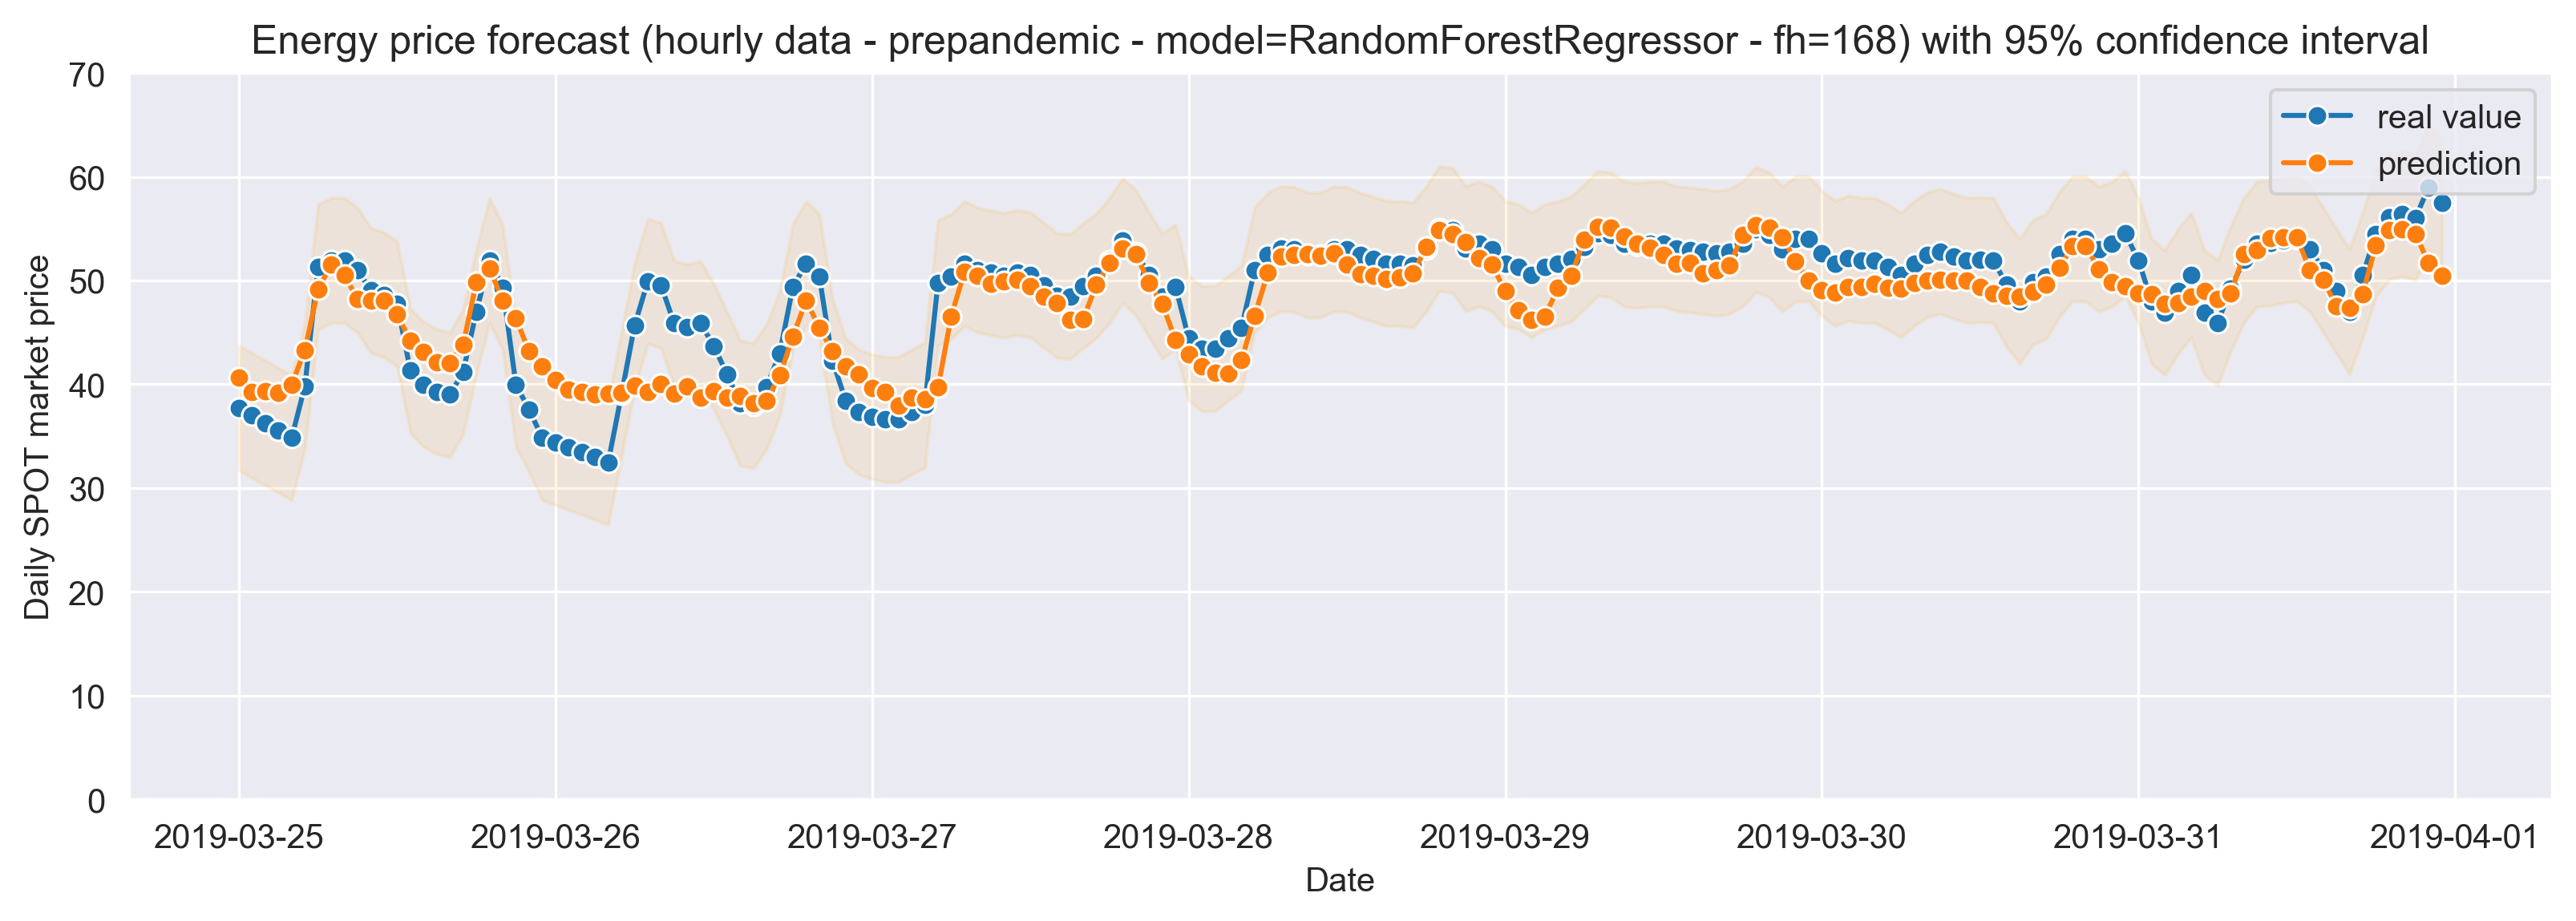
\includegraphics[scale=0.4]{images/analysis/forecast-hourly-pre}}
\end{figure}

Which are the predictors that are specially influencing this forecast? If lags are included in the SHAP study, see Figure \ref{fig:shap-hourly-pre-lags}, the first lag has a lot of importance. Concretely, if the lag takes a low value (blue color), the response value will tend to be low too, and vice-versa. Lag two has also some importance, but in this case a low value in the lag means a higher value in the response and vice-versa. The third lag with more importance is 167, specially in the positive side, when it takes a high value the output does the same.

About the rest of predictors, combined cycle generation and hour seem to have some importance. If the generation by combined cycle is high, the price goes up and vice-versa. The price in earlier hours is usually cheaper than in the end of the day: this makes sense, being correlated with the demand which is lower during the night.

Let's now train the same model without lags to see the predictor's importance more clearly (Figure \ref{fig:shap-hourly-pre-nolags}). Again, combined cycle generation and hour are between the most influential predictors. Others such as coal, nuclear and hydropower generation appear in the top too. For the nuclear case, the more generation the lower the energy price: as explained in Chapter \ref{ch:electricity-market}, nuclear plants can't be stopped, so they always bet for very low prices. The more nuclear generation, the higher the chances of getting a low price.

\begin{figure}[H]
\centering
    \begin{subfigure}[t]{.45\textwidth}
        \centering
        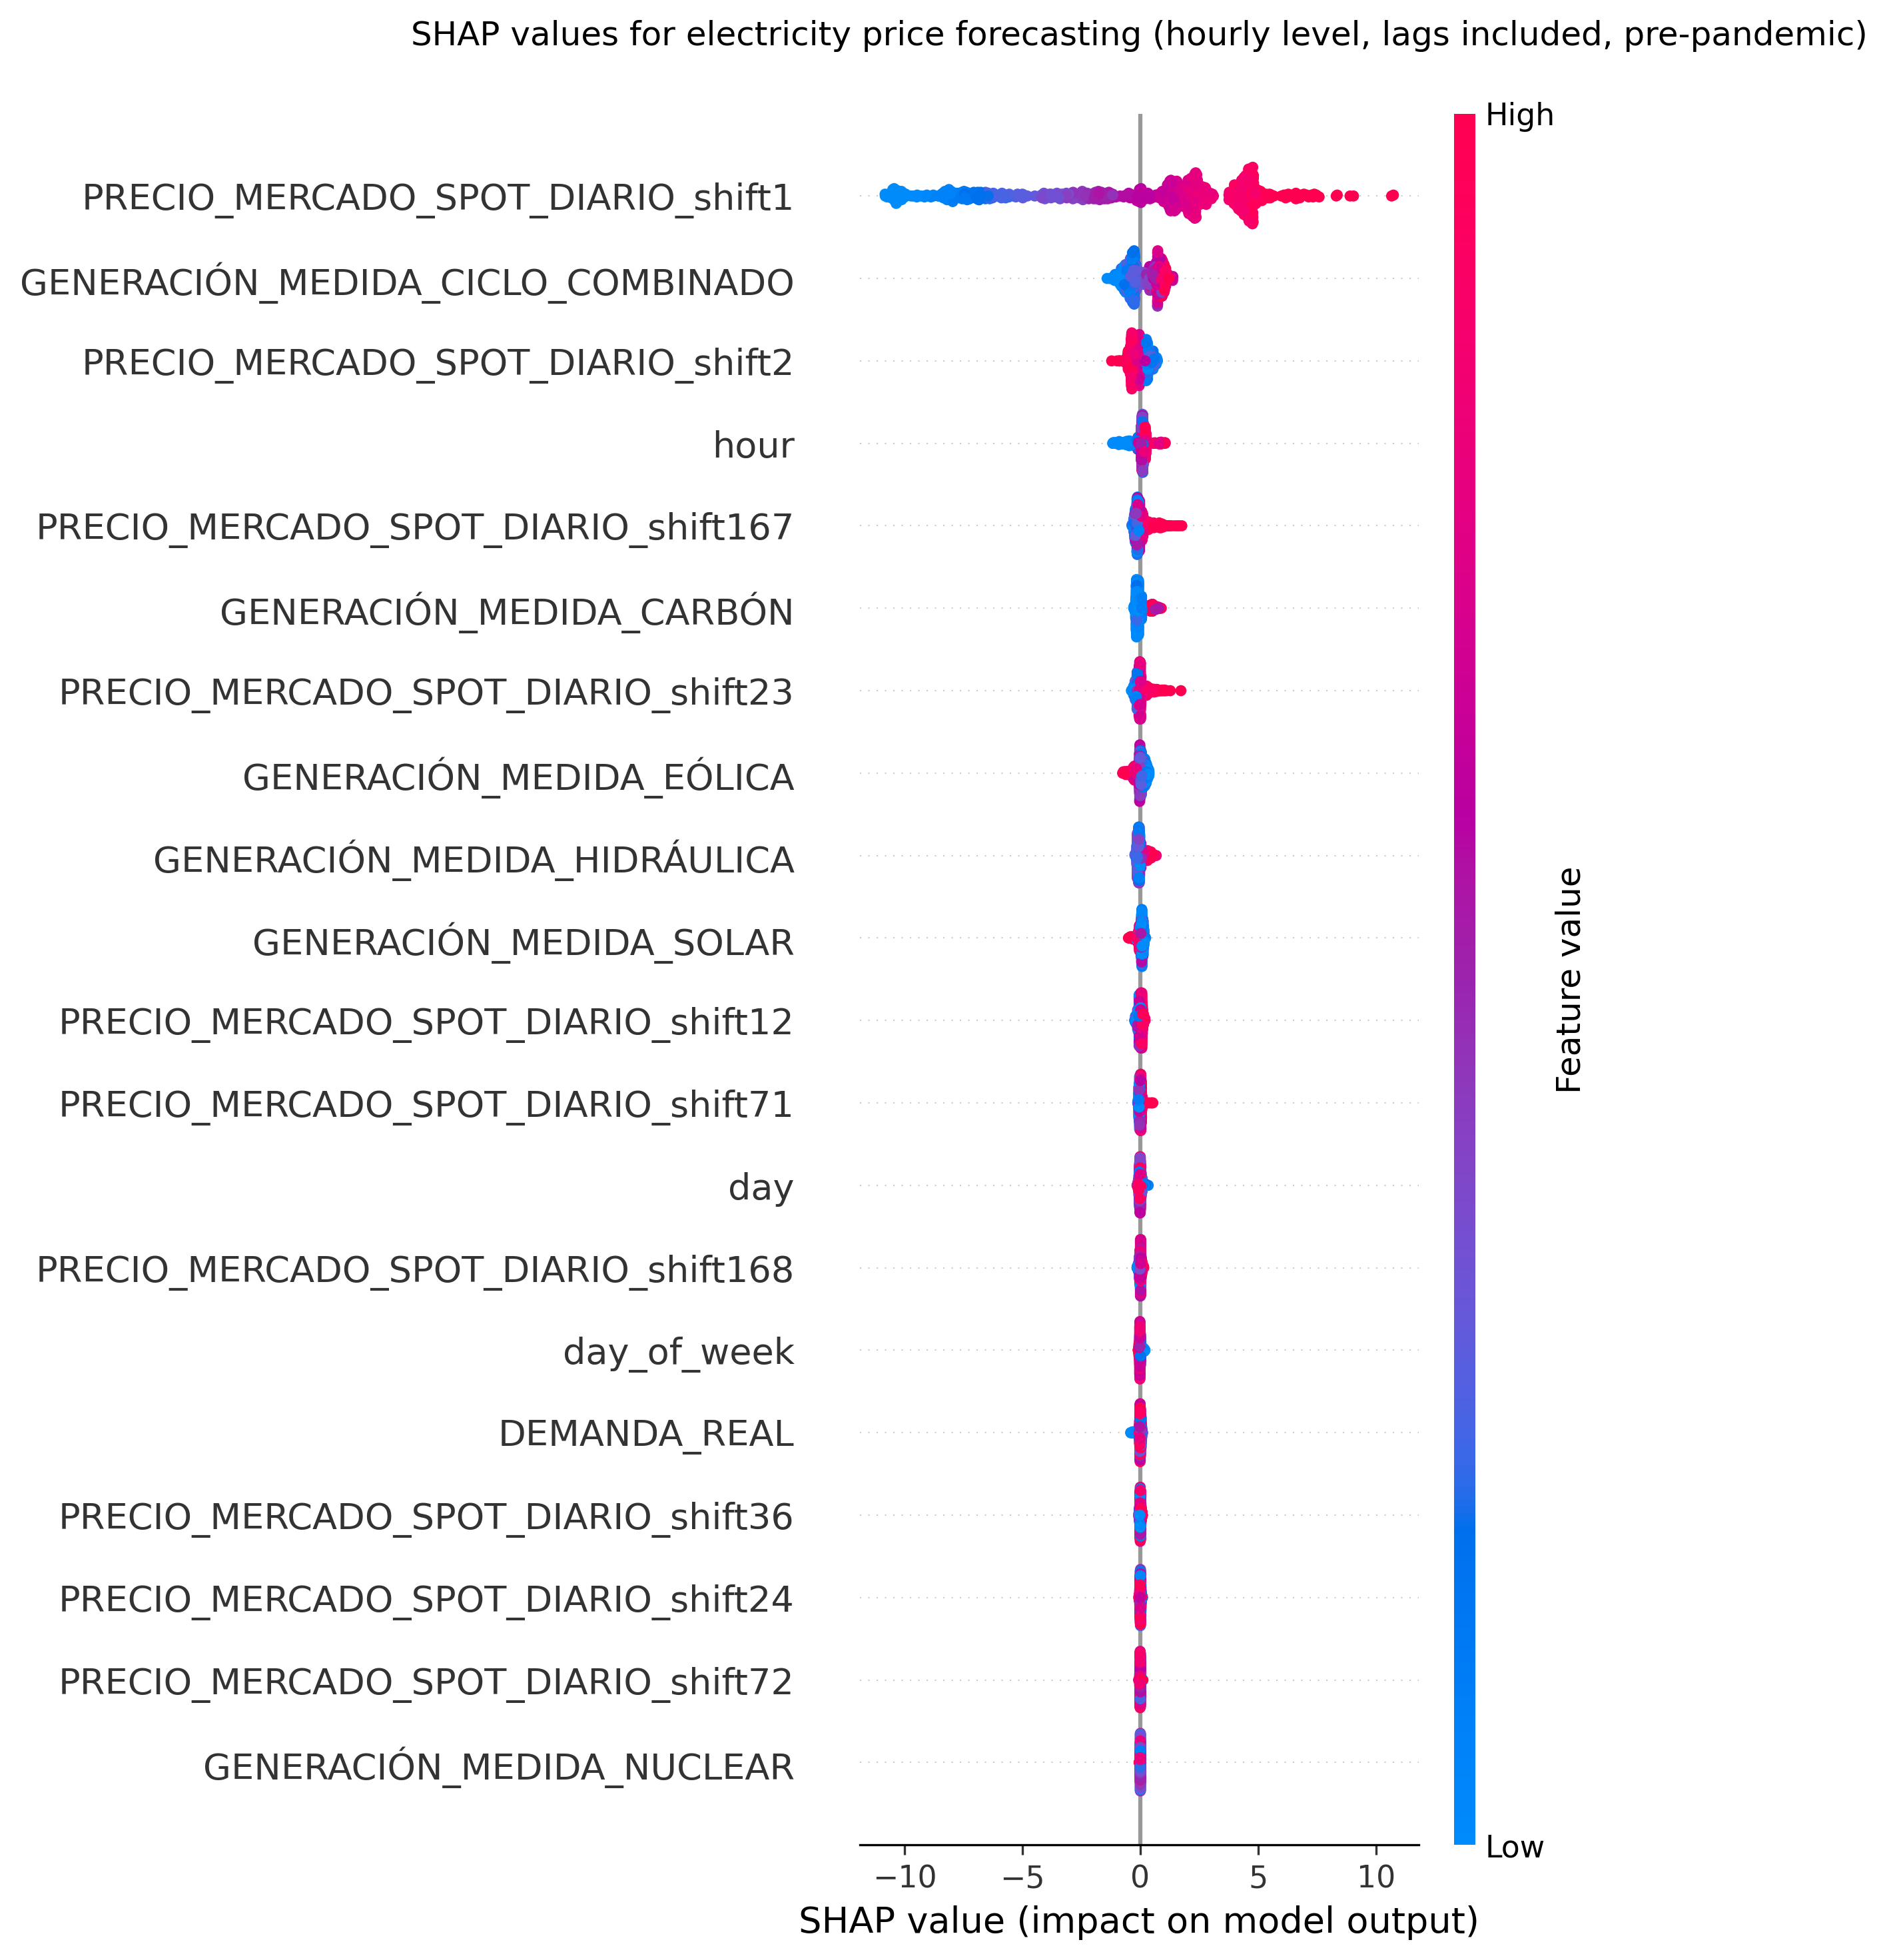
\includegraphics[width=1\linewidth]{images/analysis/shap-hourly-pre}
        \caption{SHAP values including lags.}
        \label{fig:shap-hourly-pre-lags}
    \end{subfigure}
    \begin{subfigure}[t]{.45\textwidth}
        \centering
        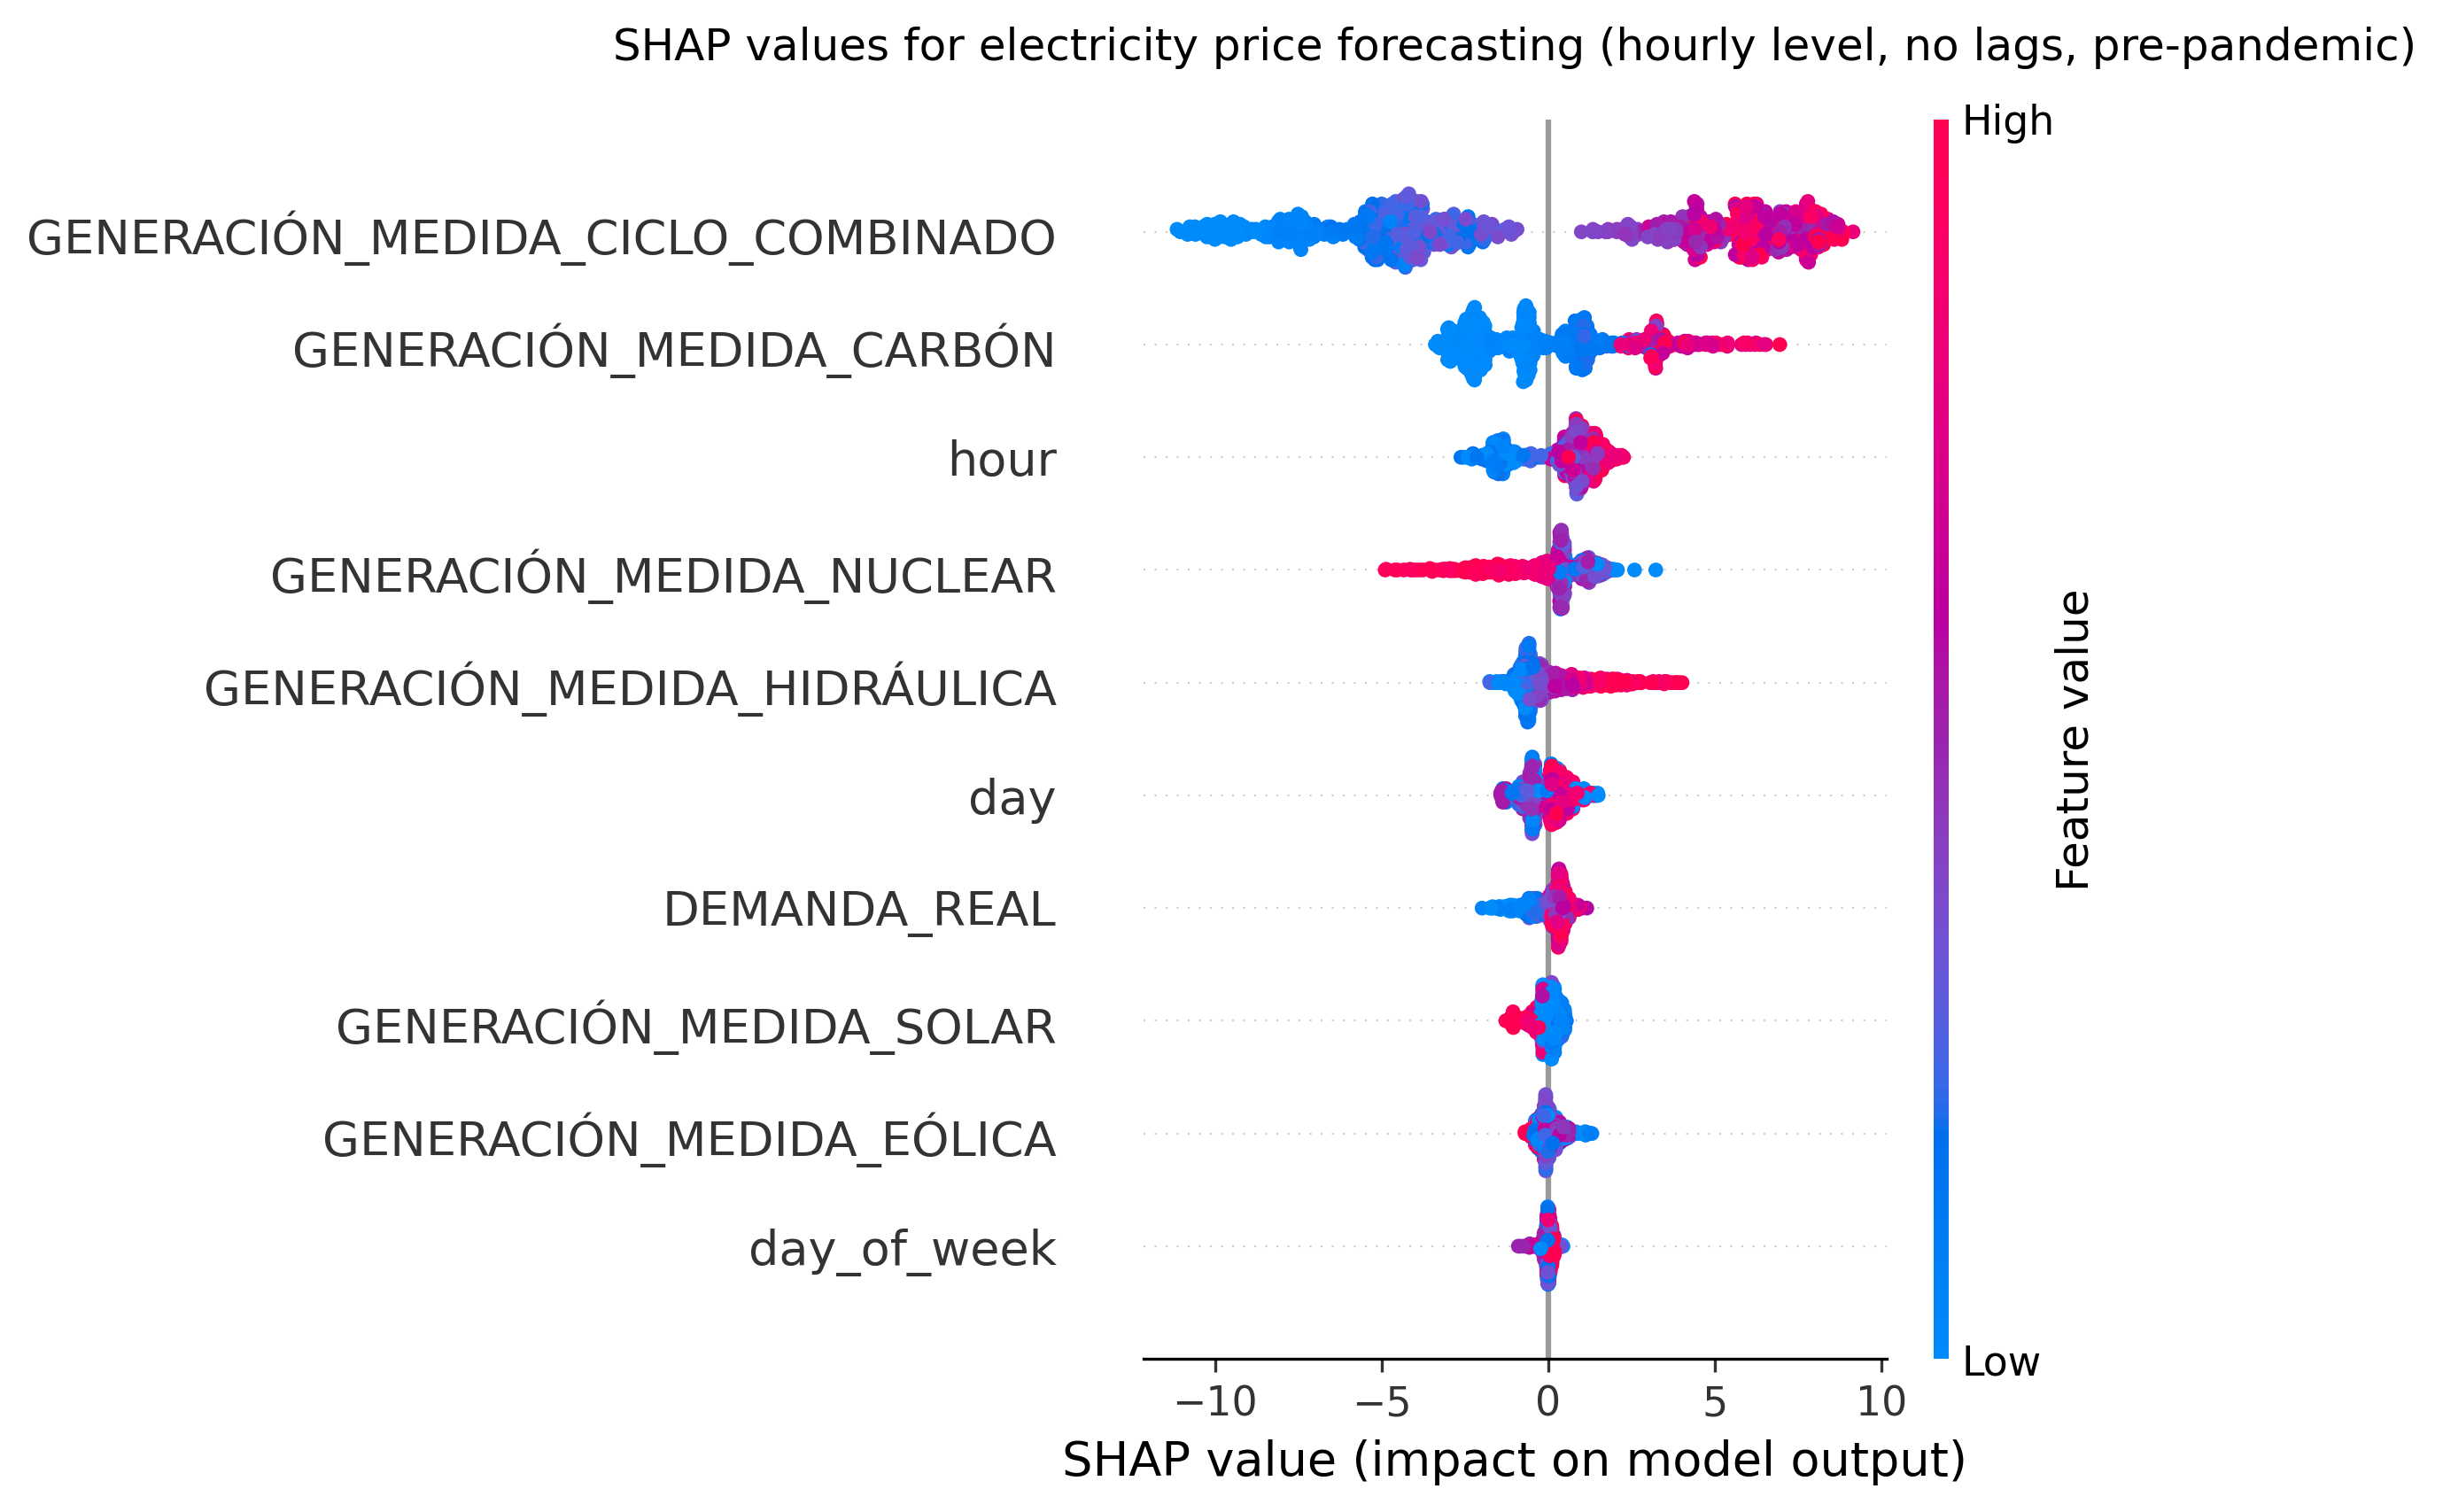
\includegraphics[width=1\linewidth]{images/analysis/shap-hourly-pre-nolags}
        \caption{SHAP values not including lags.}
        \label{fig:shap-hourly-pre-nolags}
    \end{subfigure}

    \caption{SHAP values for the hourly pre-pandemic energy price forecasting.}
    \label{fig:shap-hourly-pre}
\end{figure}

\subsection{Post-Ukraine war scenario}
The data in use goes from 2022-10-01 to 2023-03-31. In the model selection stage the author obtains the results described in Table \ref{tab:cv-hourly-post}.

% Please add the following required packages to your document preamble:
% \usepackage{booktabs}
\begin{table}[H]
\centering
\begin{tabular}{@{}l|l|l@{}}
\toprule
Model & MASE  & Modelling time (s)  \\ \midrule
RF    & 1,964 & 98.63               \\
GBT   & 2.081 & 67.17               \\
kNN   & 4.014 & 111.84              \\ \bottomrule
\end{tabular}
\caption{Model performance comparison trained over the hourly post-Ukraine war energy prices.}
\label{tab:cv-hourly-post}
\end{table}

The best-performing model, in this post-war scenario, is again the one based on Random Forests (RF). The final forecast is shown in Figure \ref{fig:forecast-hourly-post}: a final MAE of 1.702 has been obtained over the test partition. It can be checked how the model is correctly capturing the cyclicity in the data.

\begin{figure}[H]
\centering
    \caption{Final forecasting of hourly post-war energy price.}
    \label{fig:forecast-hourly-post}
    \fbox{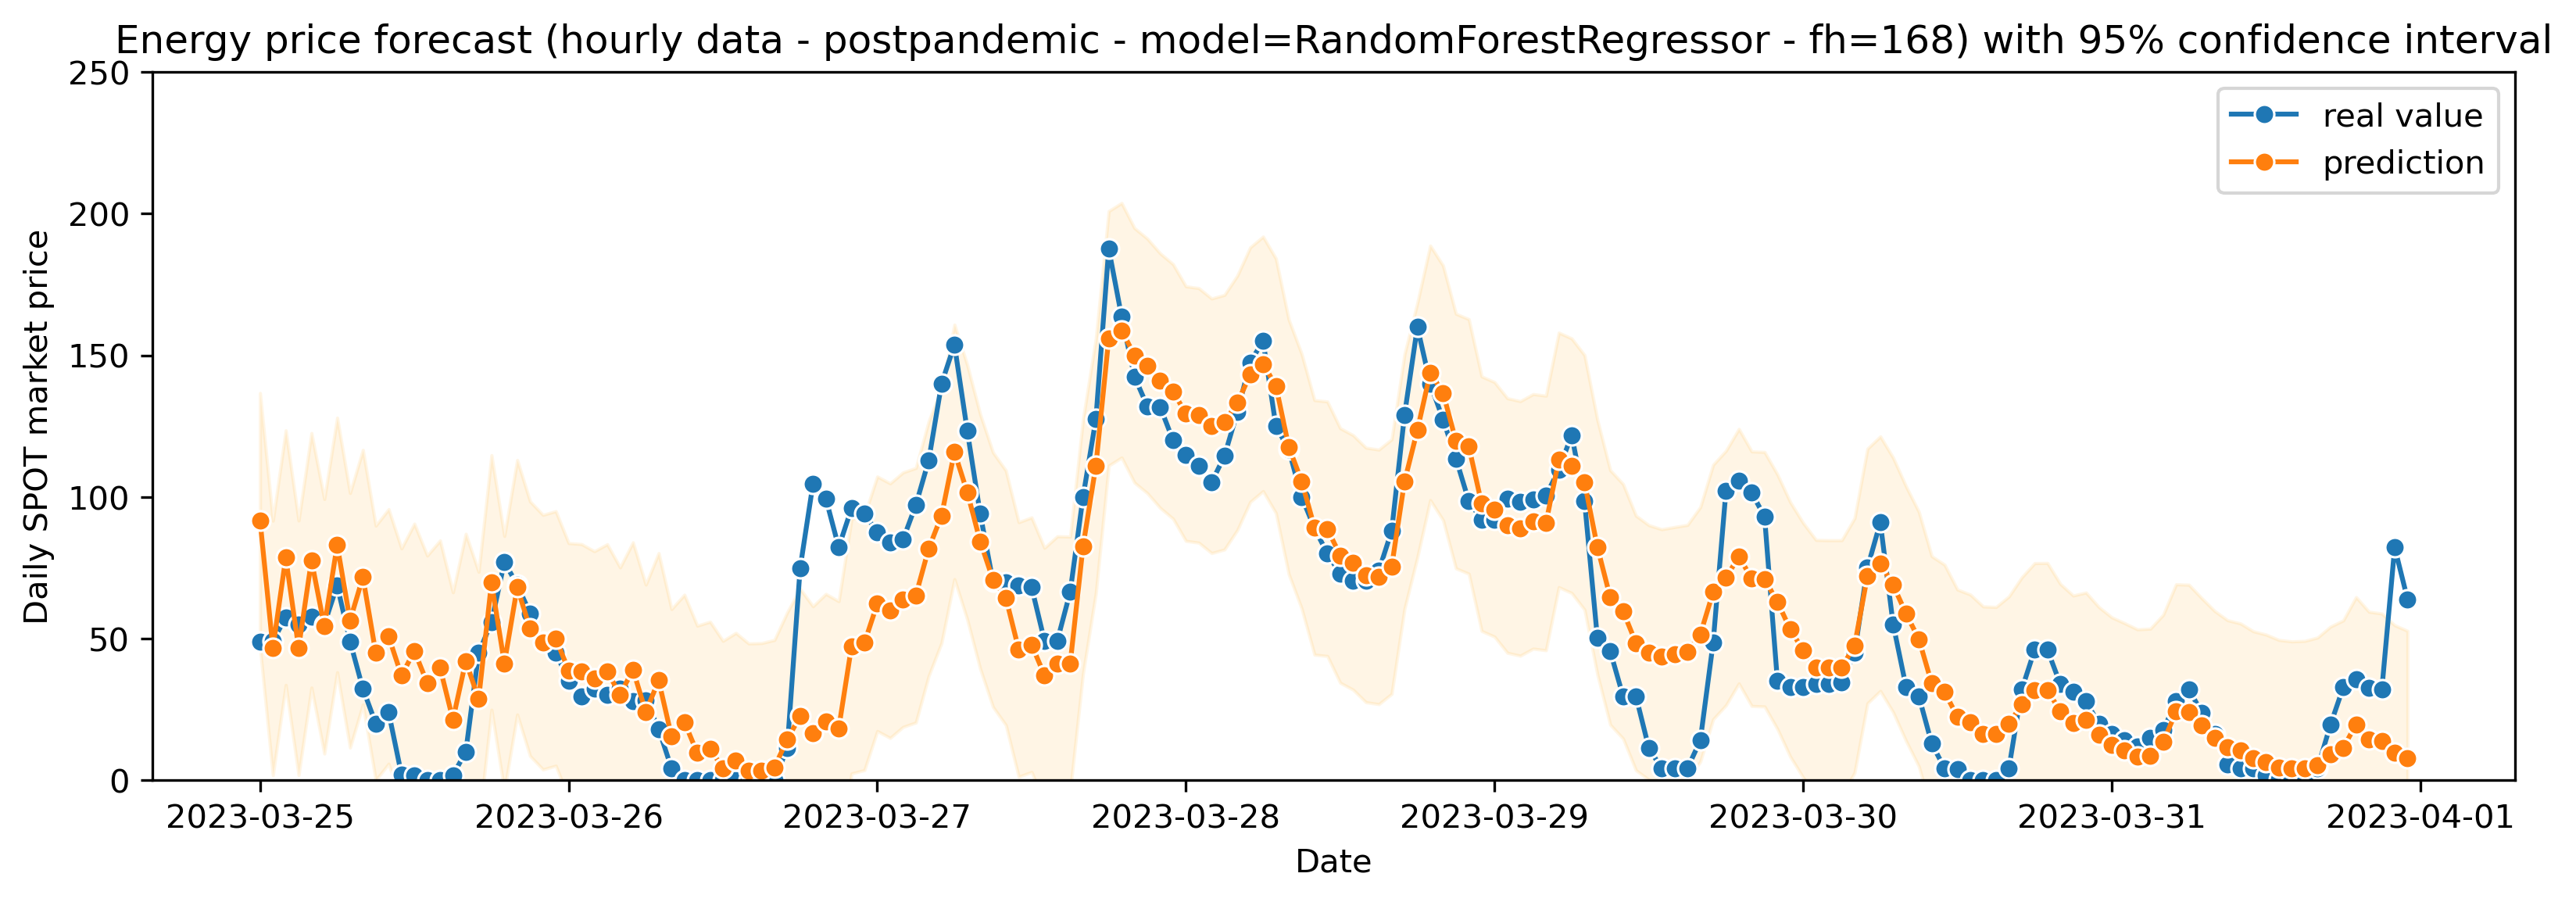
\includegraphics[scale=0.4]{images/analysis/forecast-hourly-post}}
\end{figure}

In this case, the most important predictors are shown in Figure \ref{fig:shap-hourly-post}. Compared with the pre-pandemic series, we find similar predictors. A lag which seems more important than before is 23, but in general everything is similar.

If the model without using lags is studied, the most influential variable is again combined cycle generation. It seems to be more influential than before, relatively comparing with other predictors' importance. Date predictors such as day, day or week or hour are also relevant and others such as demand, hydropower and nuclear generation.

An interesting point here is how coal generation has lost importance compared to previous years: this makes sense, as coal is less and less used as it is highly polluting. Check Figure \ref{fig:coal-series} and see how is almost irrelevant from 2019 onwards.

\begin{figure}[H]
\centering
    \begin{subfigure}{.45\textwidth}
        \centering
        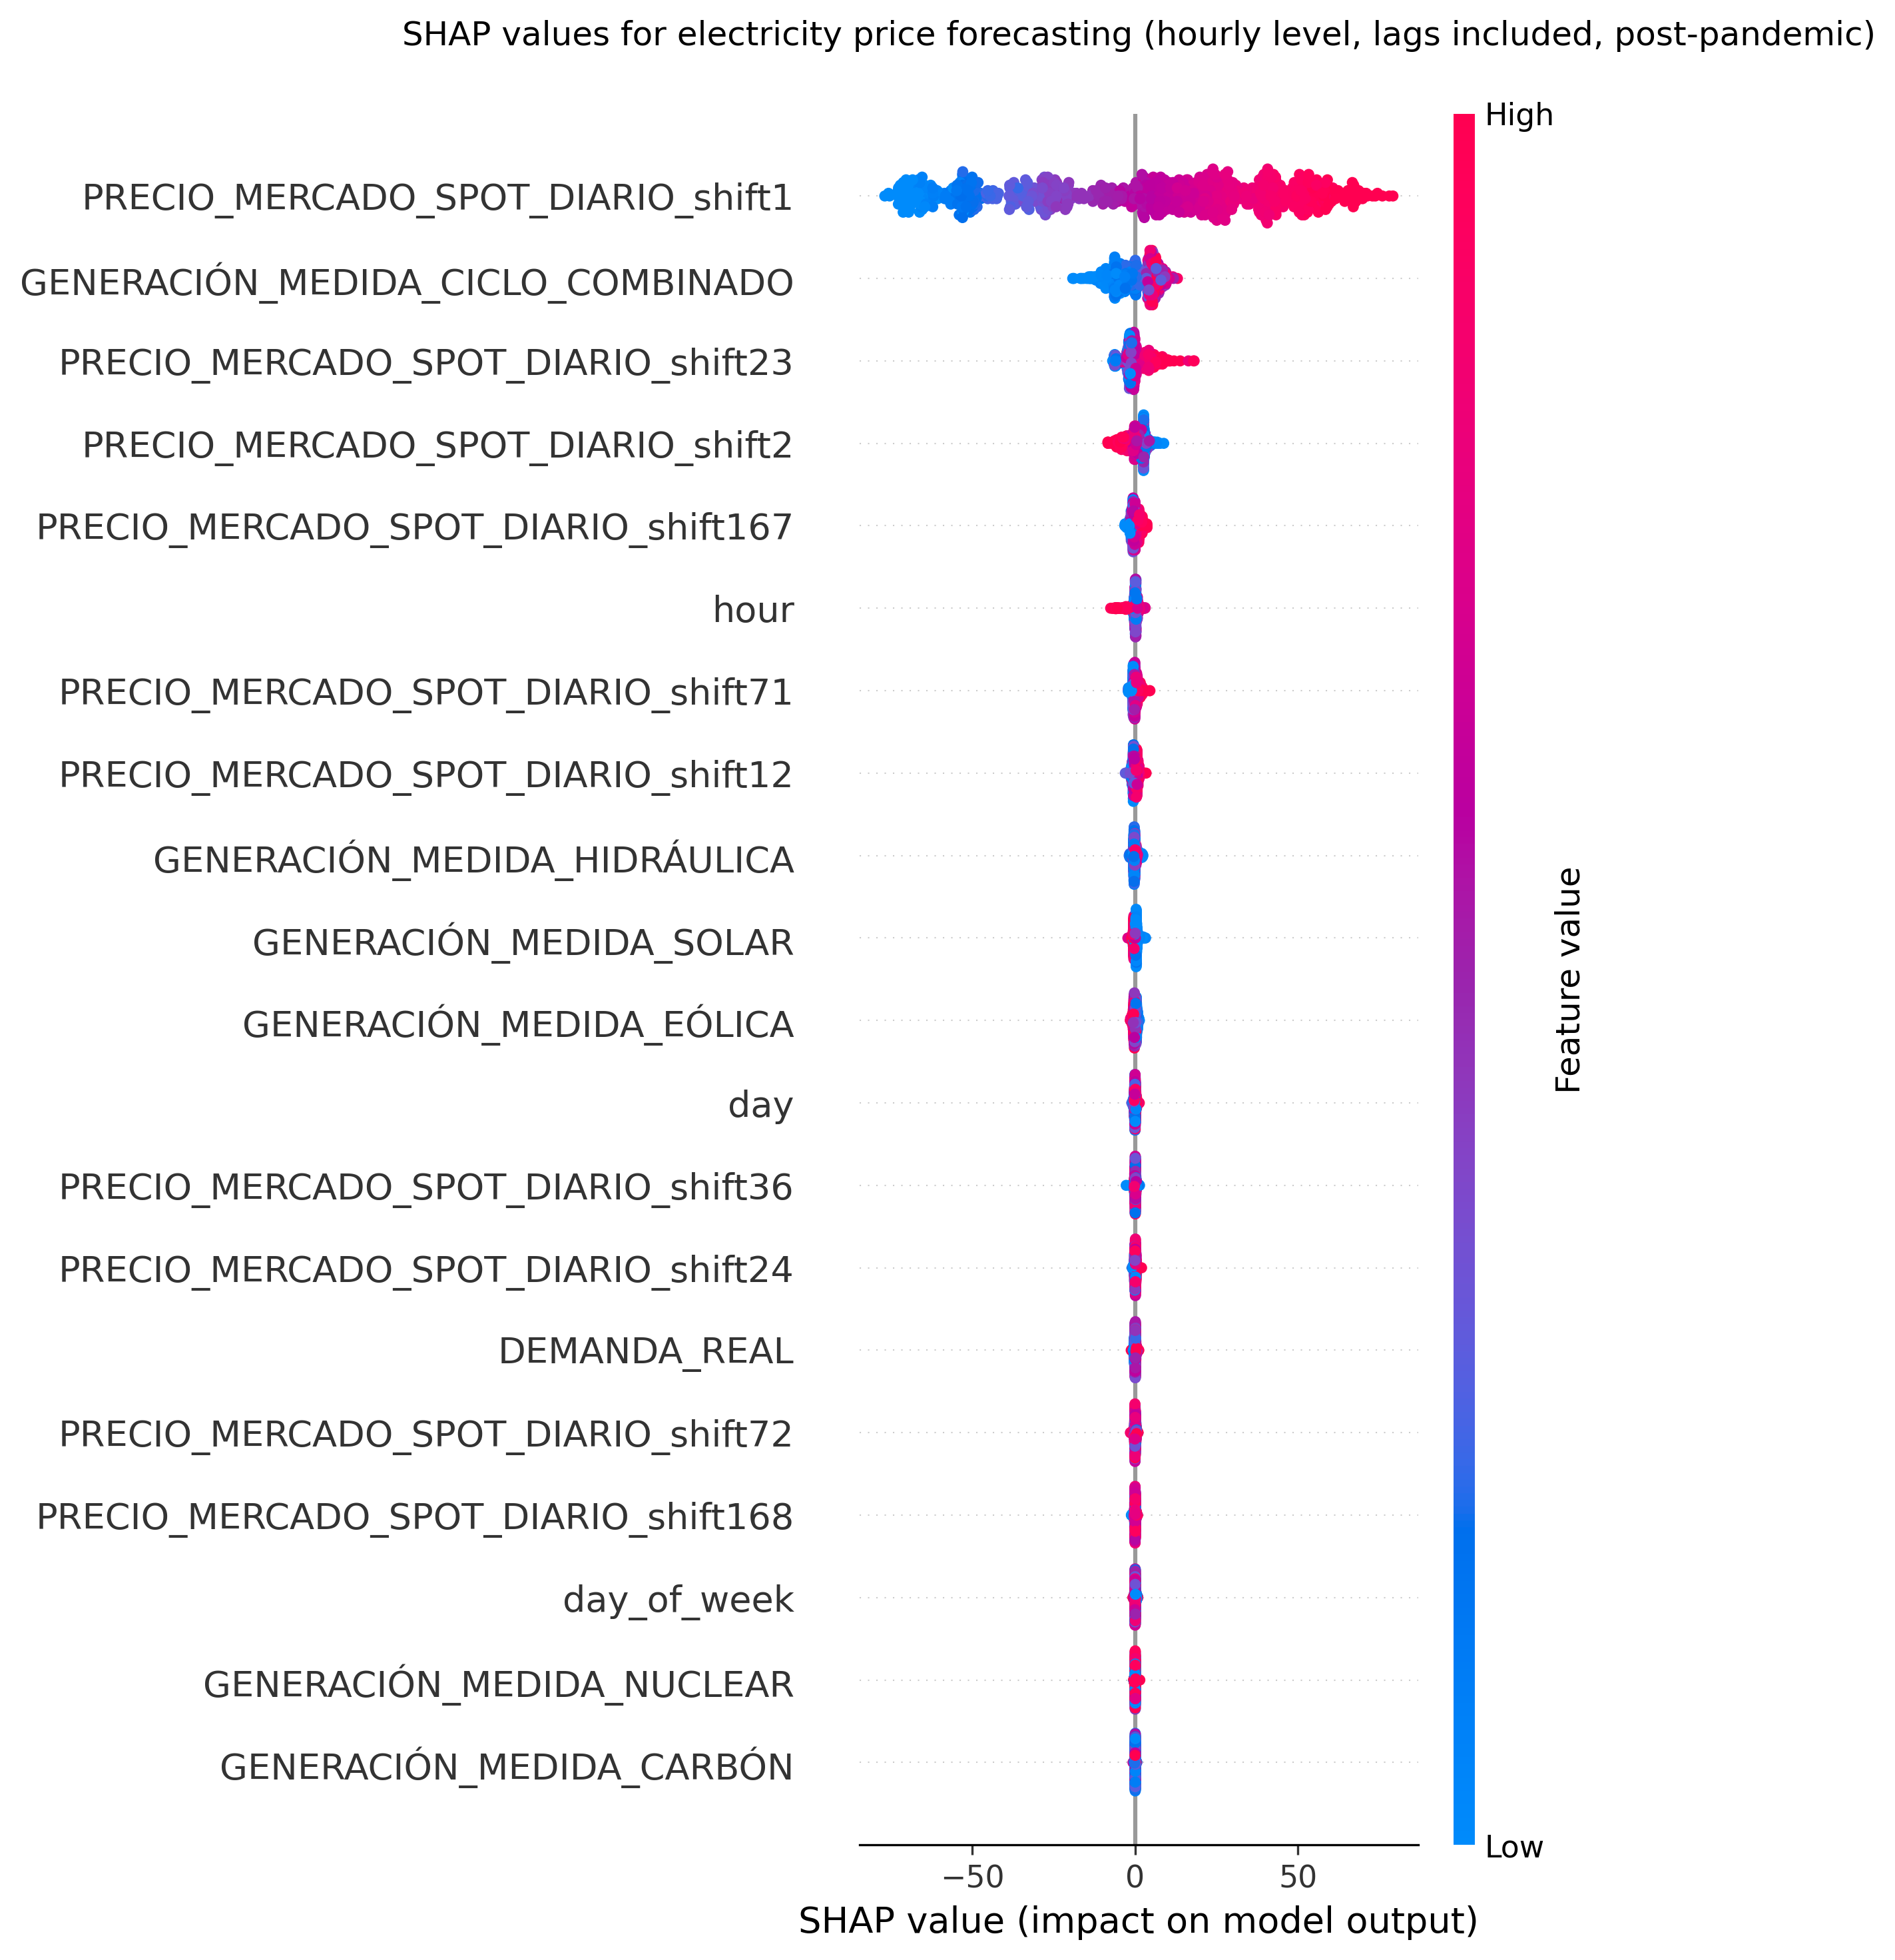
\includegraphics[width=1\linewidth]{images/analysis/shap-hourly-post}
        \caption{SHAP values including lags as predictors.}
        \label{fig:shap-hourly-post-lags}
    \end{subfigure}
    \begin{subfigure}{.45\textwidth}
        \centering
        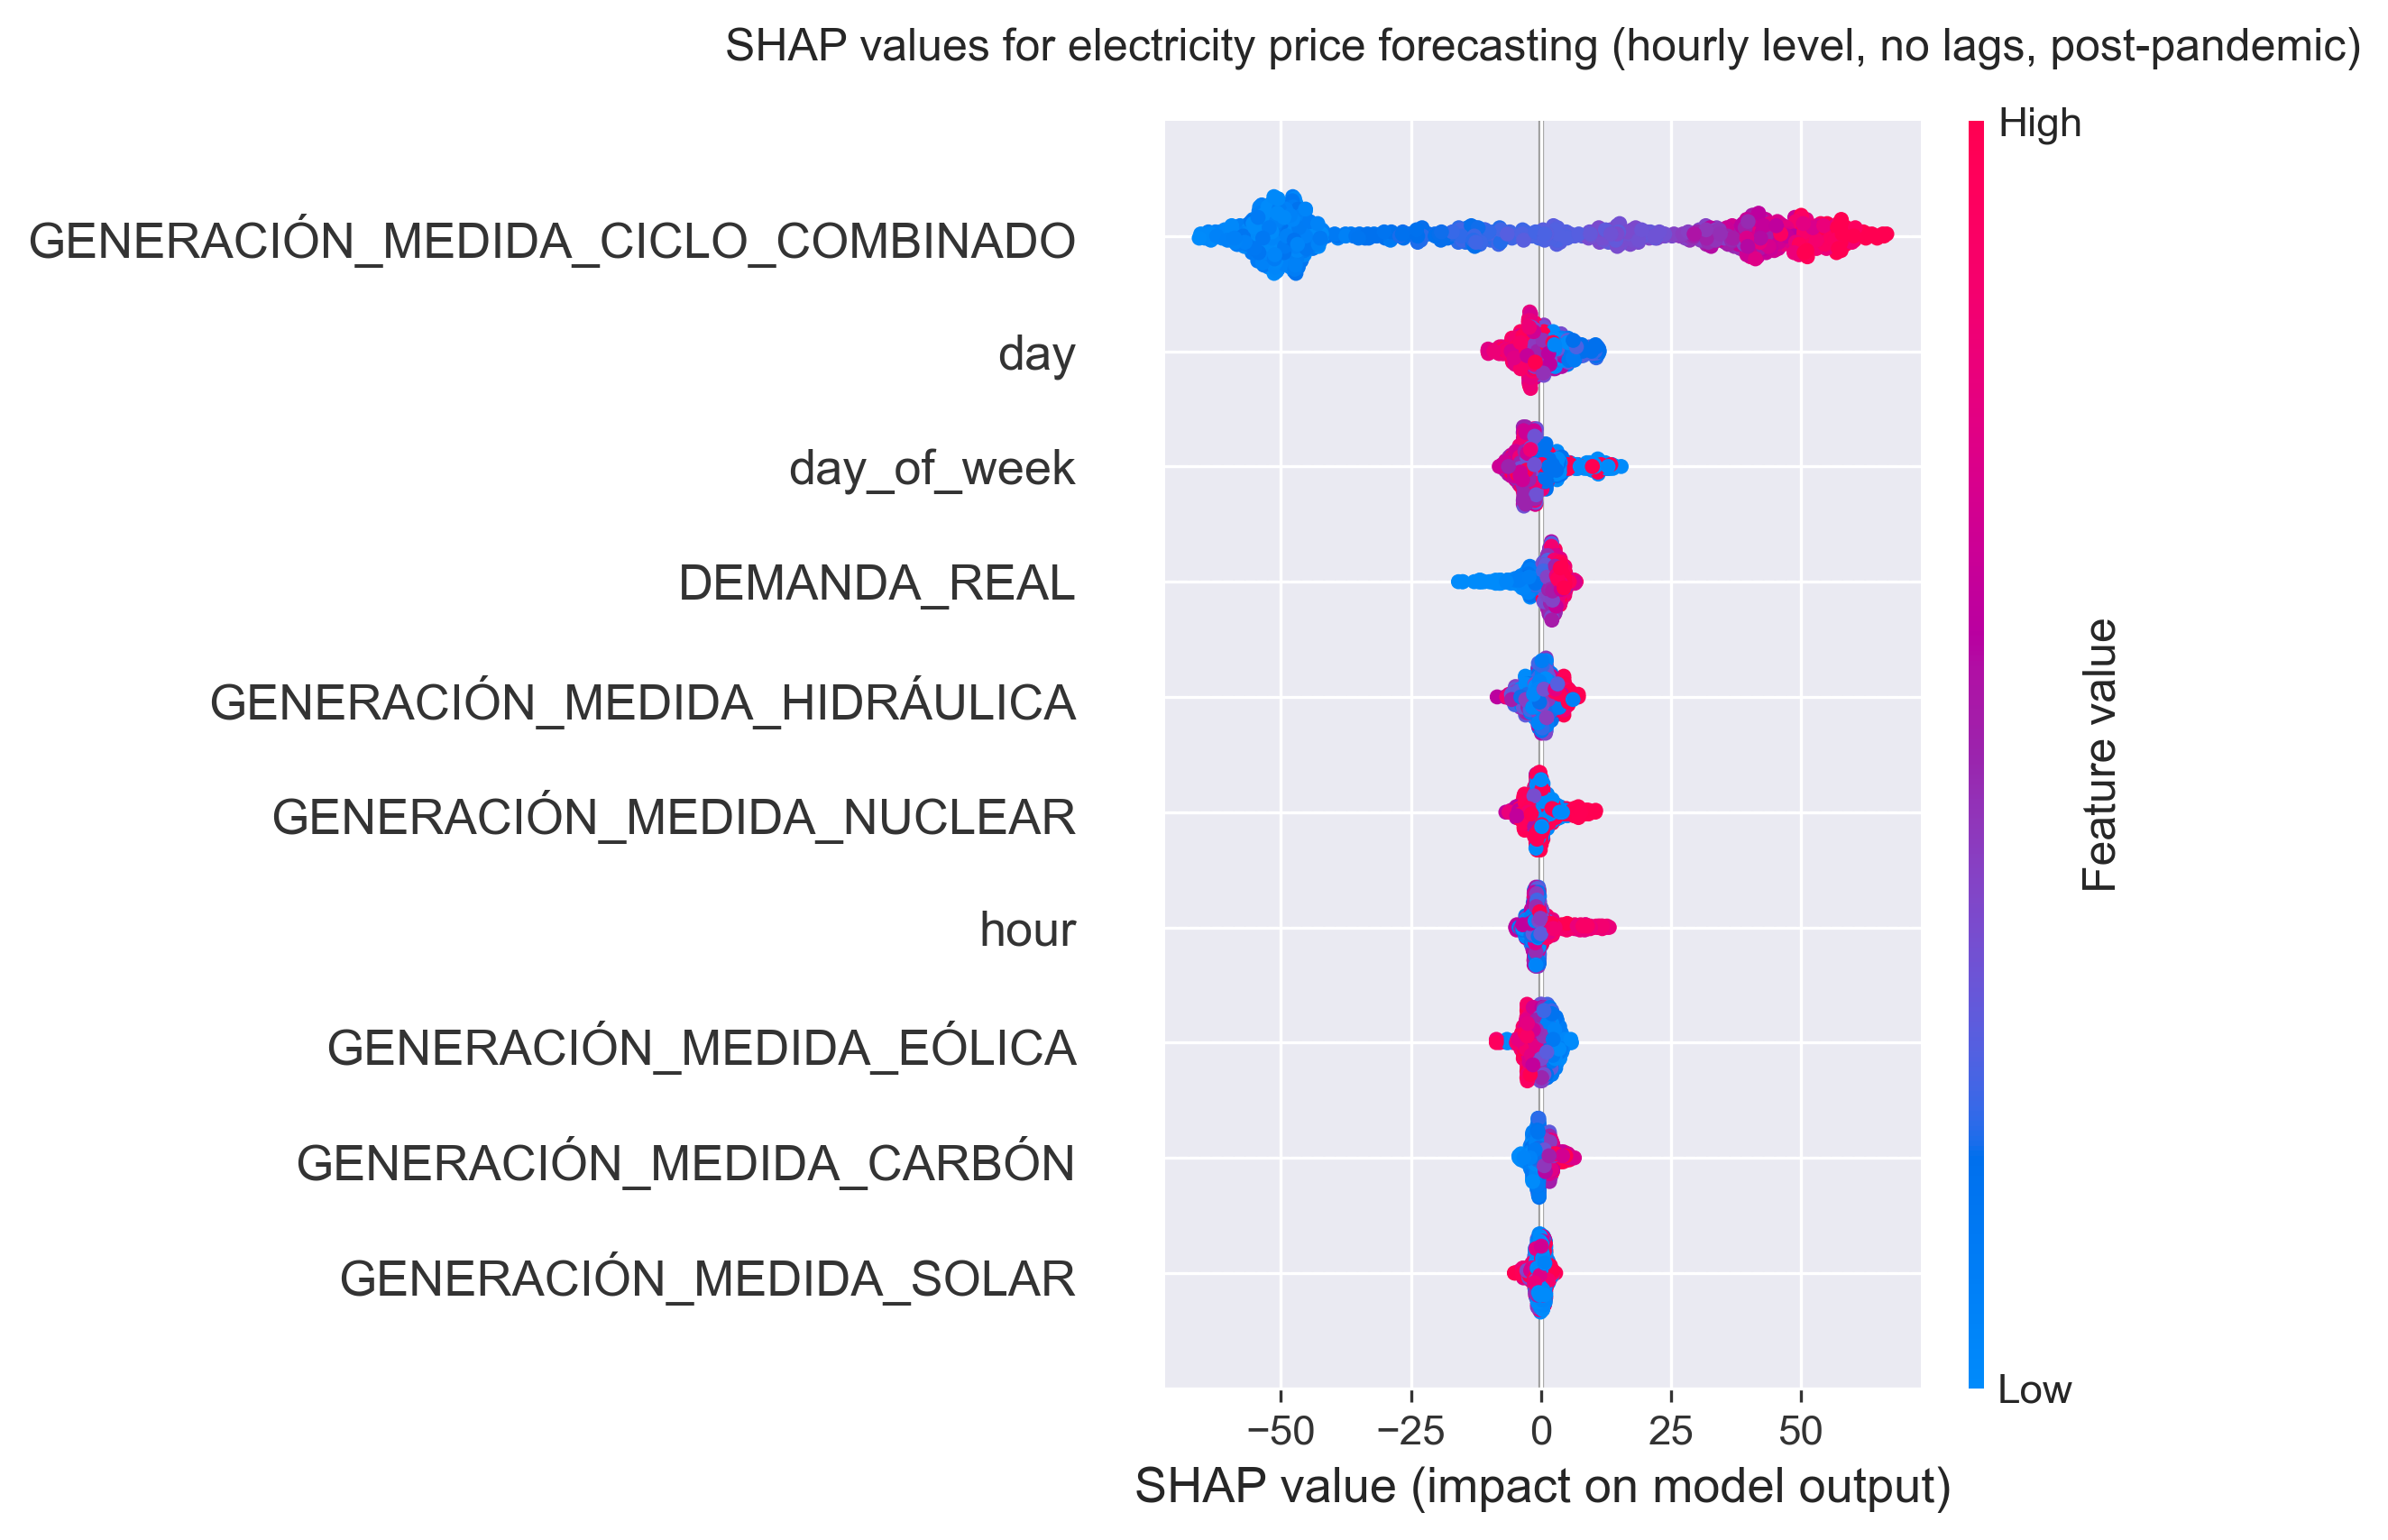
\includegraphics[width=1\linewidth]{images/analysis/shap-hourly-post-nolags}
        \caption{SHAP values not including lags as predictors.}
        \label{fig:shap-hourly-post-nolags}
    \end{subfigure}

    \caption{SHAP values for the hourly post-pandemic energy price forecasting.}
    \label{fig:shap-hourly-post}
\end{figure}

\subsection{Result discussion}
Both for the pre-pandemic and post-war scenarios the best performing models are Random Forests. Looking at the forecasts graphs, they are correctly capturing the cyclicity present in data.

An important conclusion on this study is that combined cycle generation is a relevant predictor to model hourly prices. This makes sense, because as described in Chapter \ref{ch:electricity-market}, the commodity-based technologies normally set the energy price. In the post-war market it has even gained more importance. Also, it can be seen how coal generation has lost importance in the past years, to the extent that it is hardly used today.


\newpage
\section{Daily analysis}
For the daily aggregation analysis 2 years of data are used, producing 30 days ahead forecasts. The lags added as predictors are 1, 2, 6, 7, 13, 14, 28, 30 and 31, apart we use the following new predictors:

\begin{itemize}
    \item \textbf{Date predictors:} Day, day of week, week of the year and month.
    \item \textbf{Gas price}
    \item \textbf{Coal price}
    \item \textbf{EU $CO_2$ allowances price}
\end{itemize}

\noindent Cross validation is applied again using 15 windows, but in this case the step size is 13.

\subsection{Pre-pandemic scenario}
The data used for the pre-pandemic scenario experiments ranges from 2018-04-01 to 2020-03-31. The model which performed the best was based on Gradient Boosting Trees (GBT), obtaining 1.044 as MASE, as can be seen in Table \ref{tab:cv-daily-prep}.

\begin{table}[H]
\centering
\begin{tabular}{@{}l|l|l@{}}
\toprule
Model & MASE  & Modelling time (s)  \\ \midrule
GBT   & 1.394 & 110.12 \\
RF    & 1.579 & 99.21  \\
kNN   & 1.965 & 156.20 \\ \bottomrule
\end{tabular}
\caption{Model performance comparison trained over the daily pre-pandemic energy price.}
\label{tab:cv-daily-prep}
\end{table}

The final forecast generated using GBT over holdout returns a MASE score of 1.043. The result can be visualized in Figure \ref{fig:forecast-daily-pre}: most of the true values remain inside the confidence interval generated during the forecast.

\begin{figure}[H]
\centering
    \caption{Final forecasting of daily pre-pandemic energy price.}
    \label{fig:forecast-daily-pre}
    \fbox{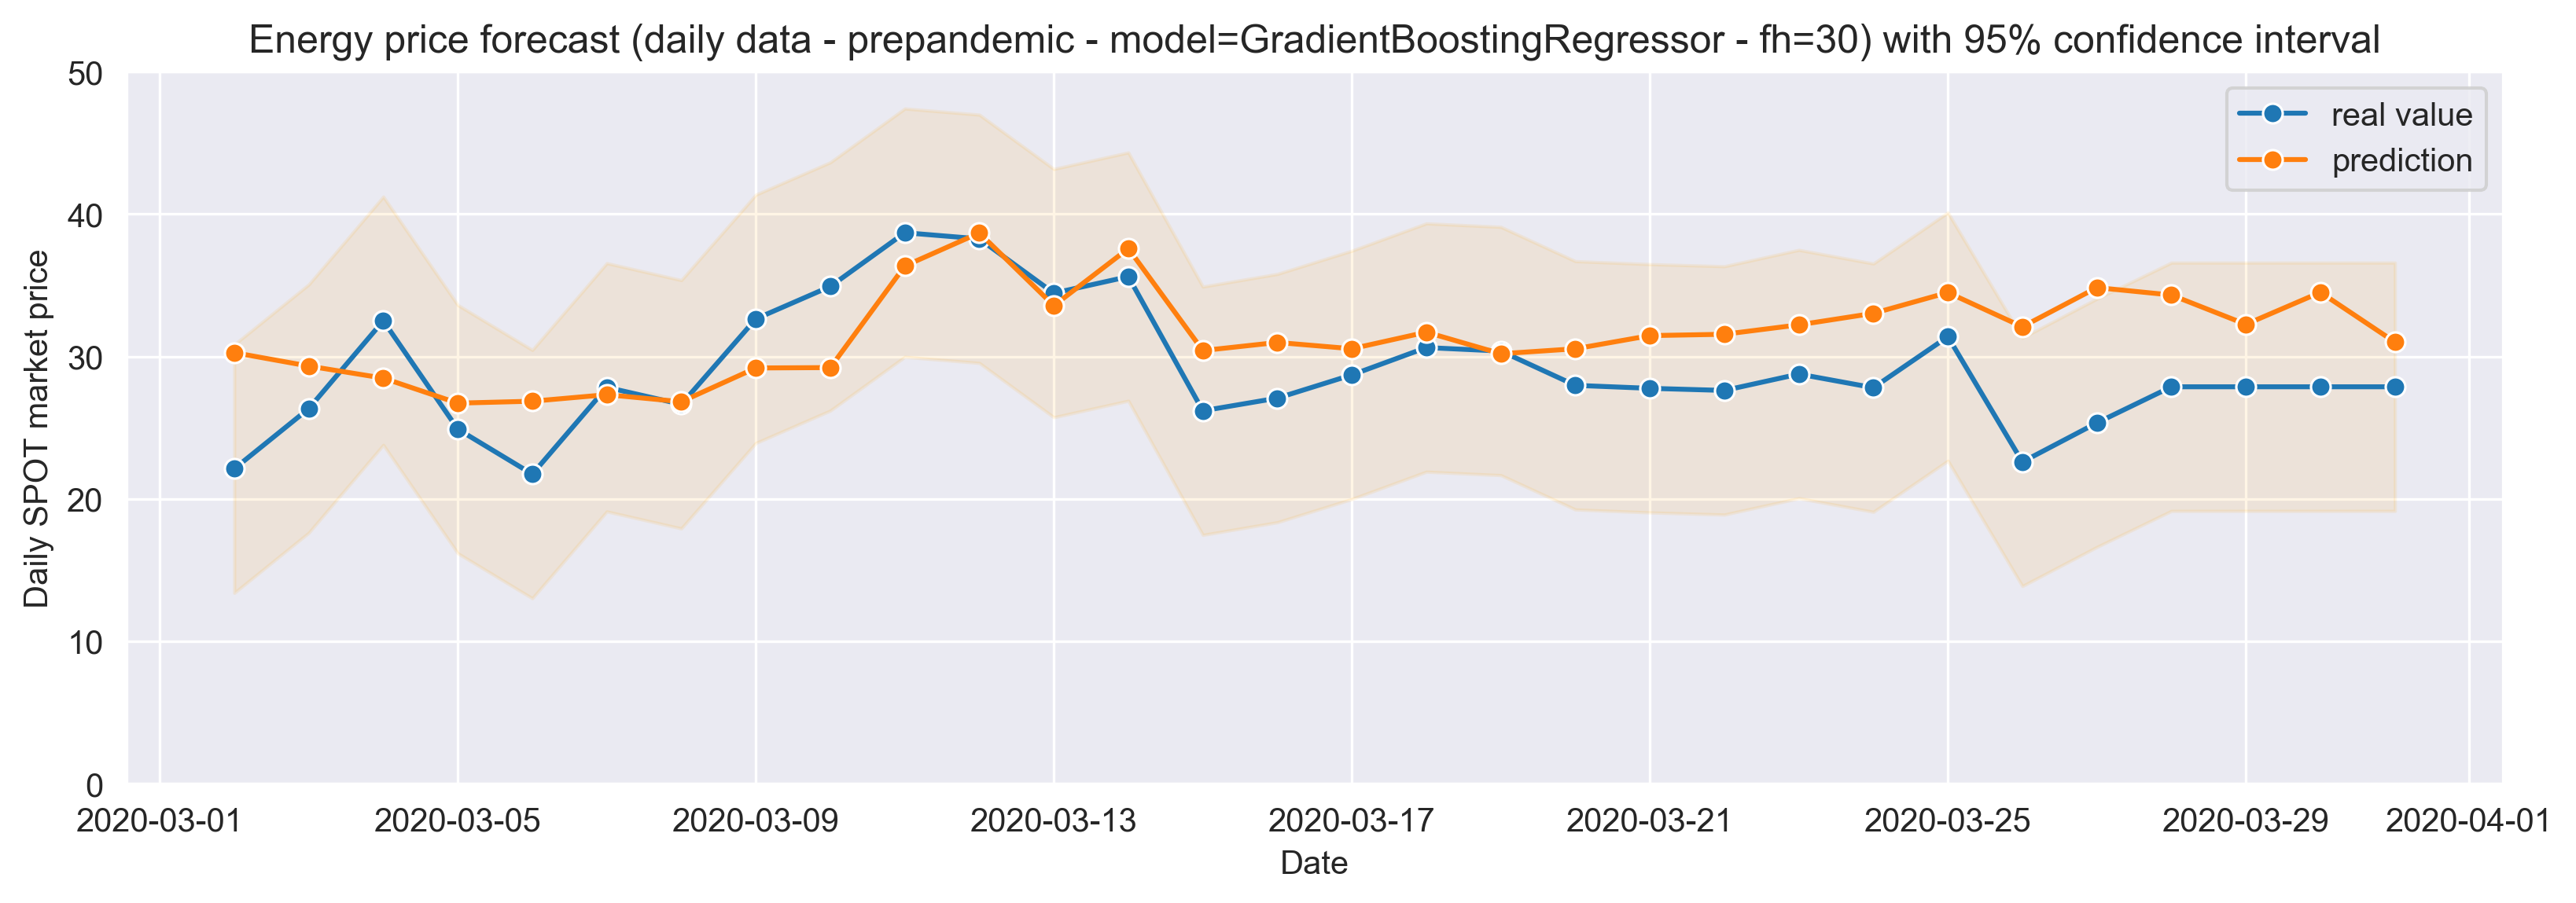
\includegraphics[scale=0.4]{images/analysis/forecast-daily-pre}}
\end{figure}

Let's now compute the SHAP values for this model. Again, we will analyze the case in which we use all the predictors (including lags) and the situation in which lags are excluded.

\begin{figure}[H]
\centering
    \begin{subfigure}{.45\textwidth}
        \centering
        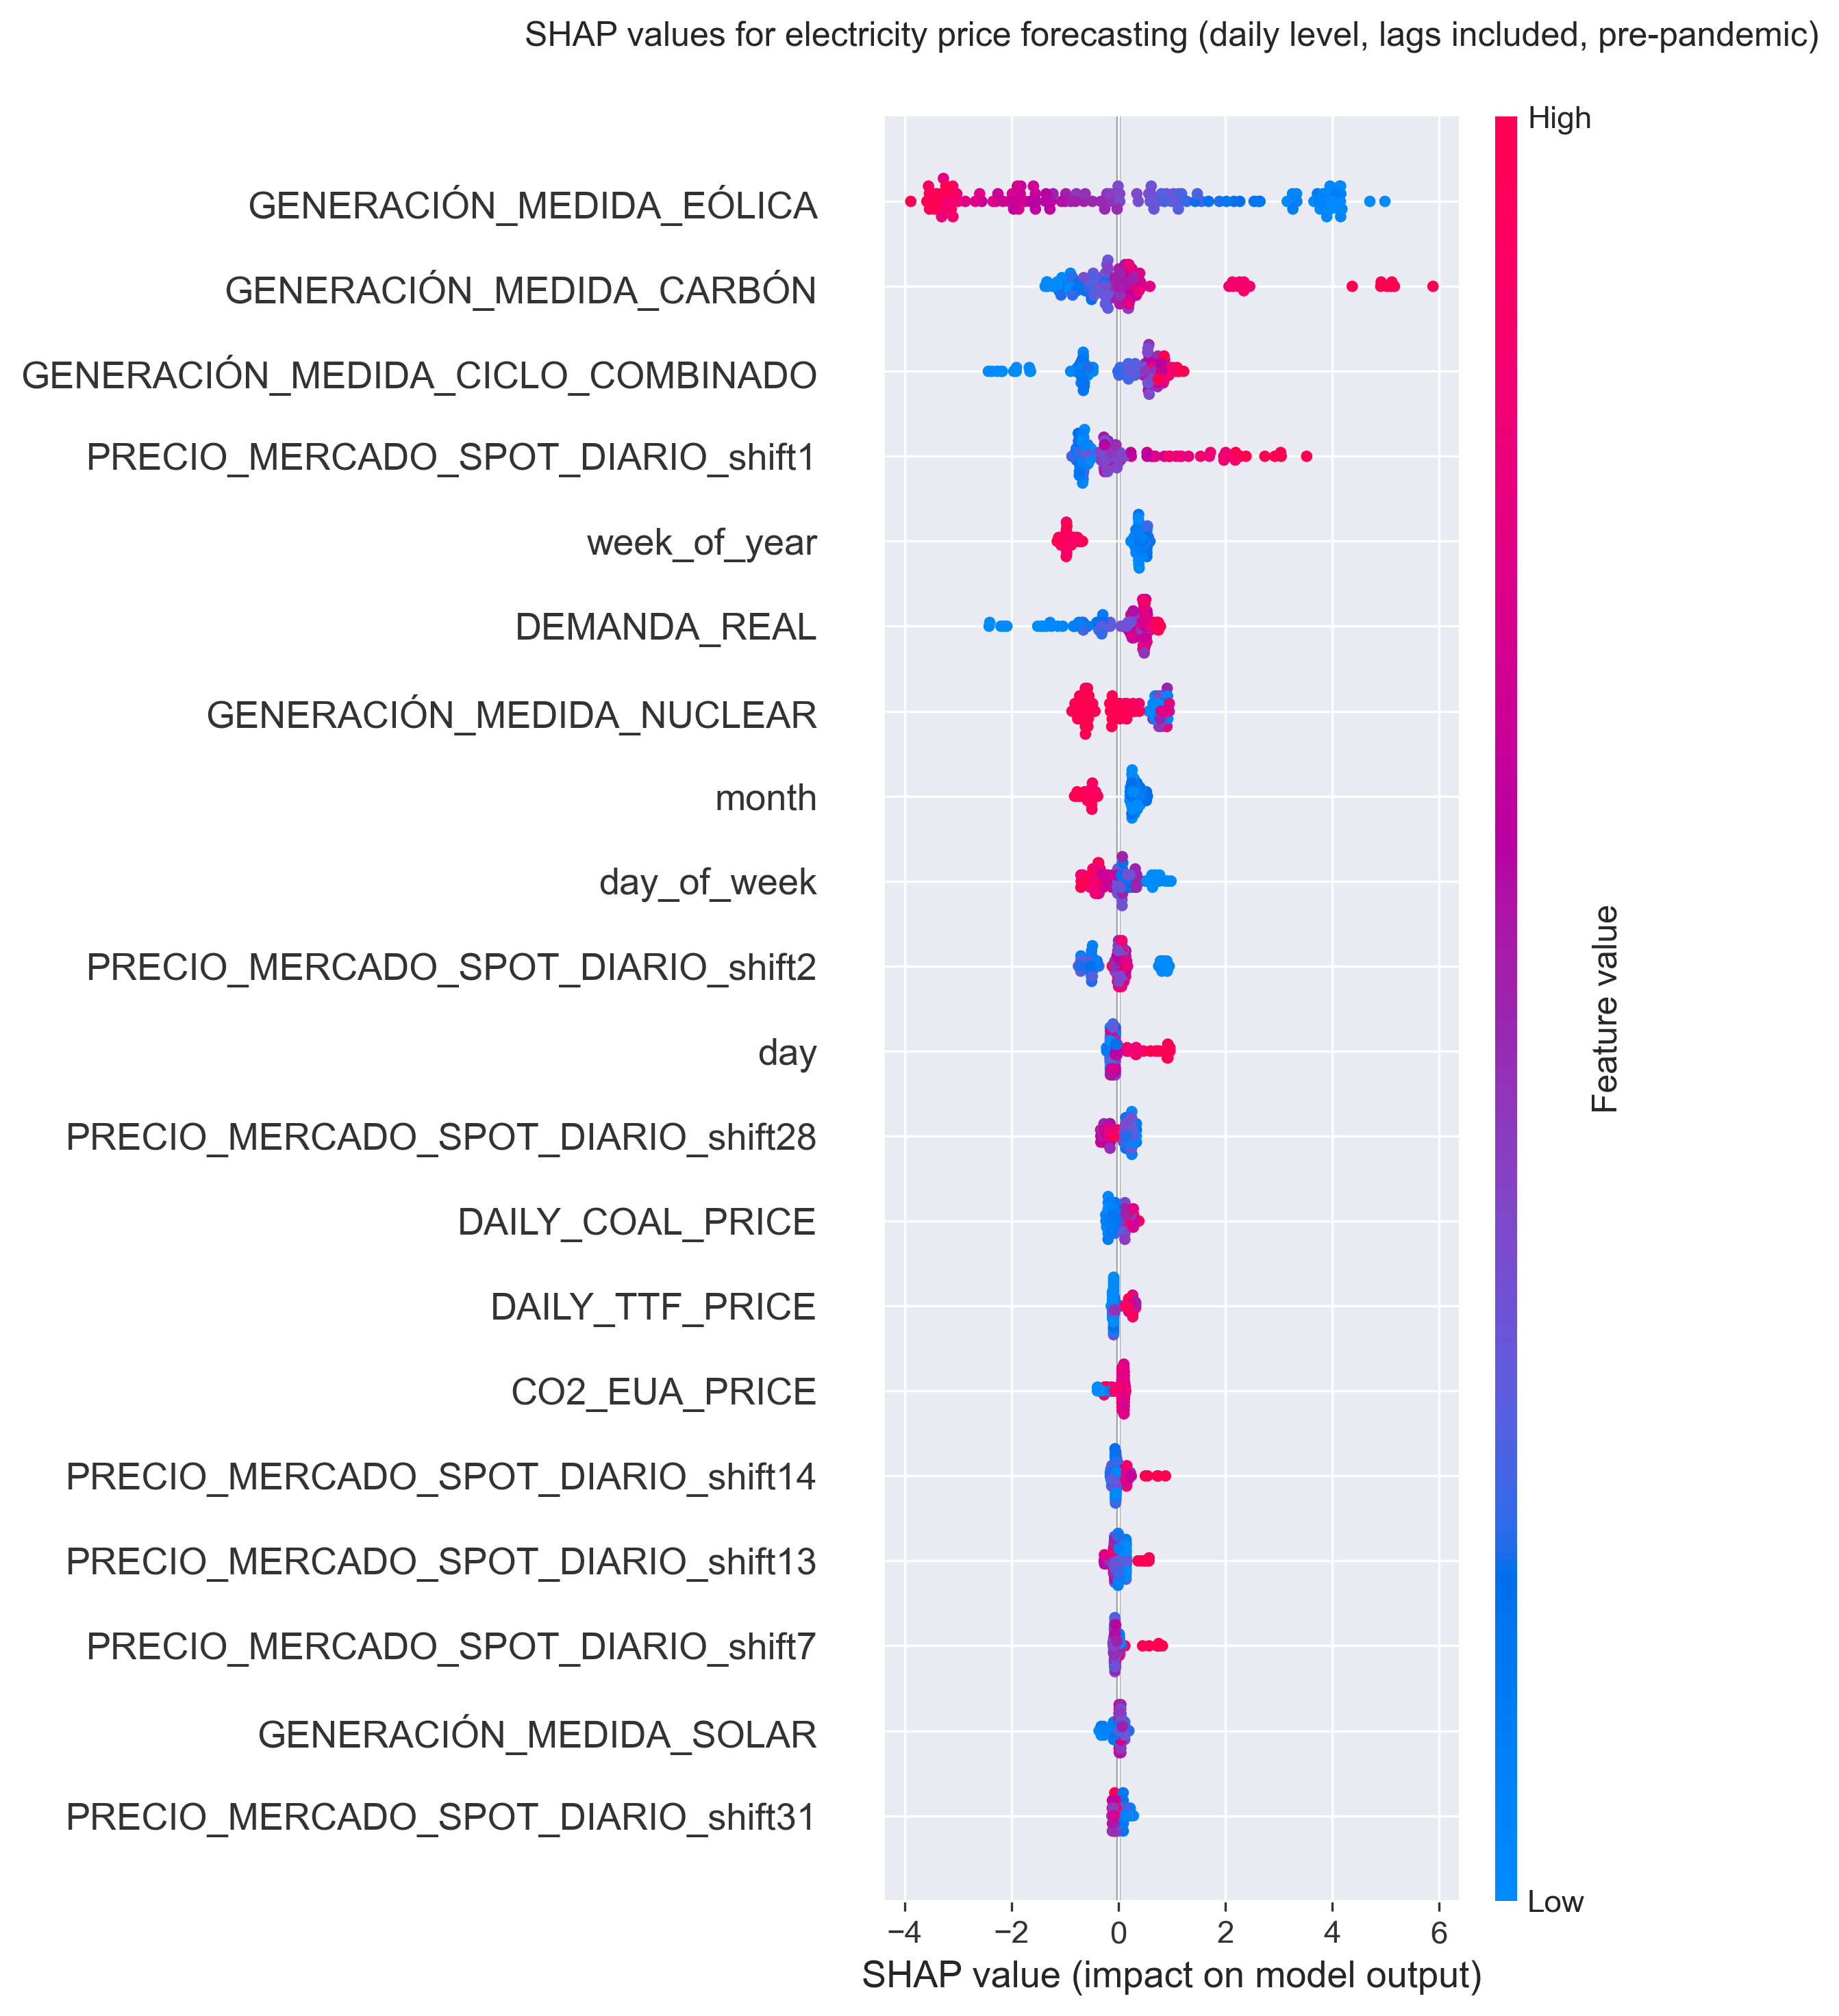
\includegraphics[width=1\linewidth]{images/analysis/shap-daily-pre}
        \caption{fh=1}
    \end{subfigure}
    \begin{subfigure}{.45\textwidth}
        \centering
        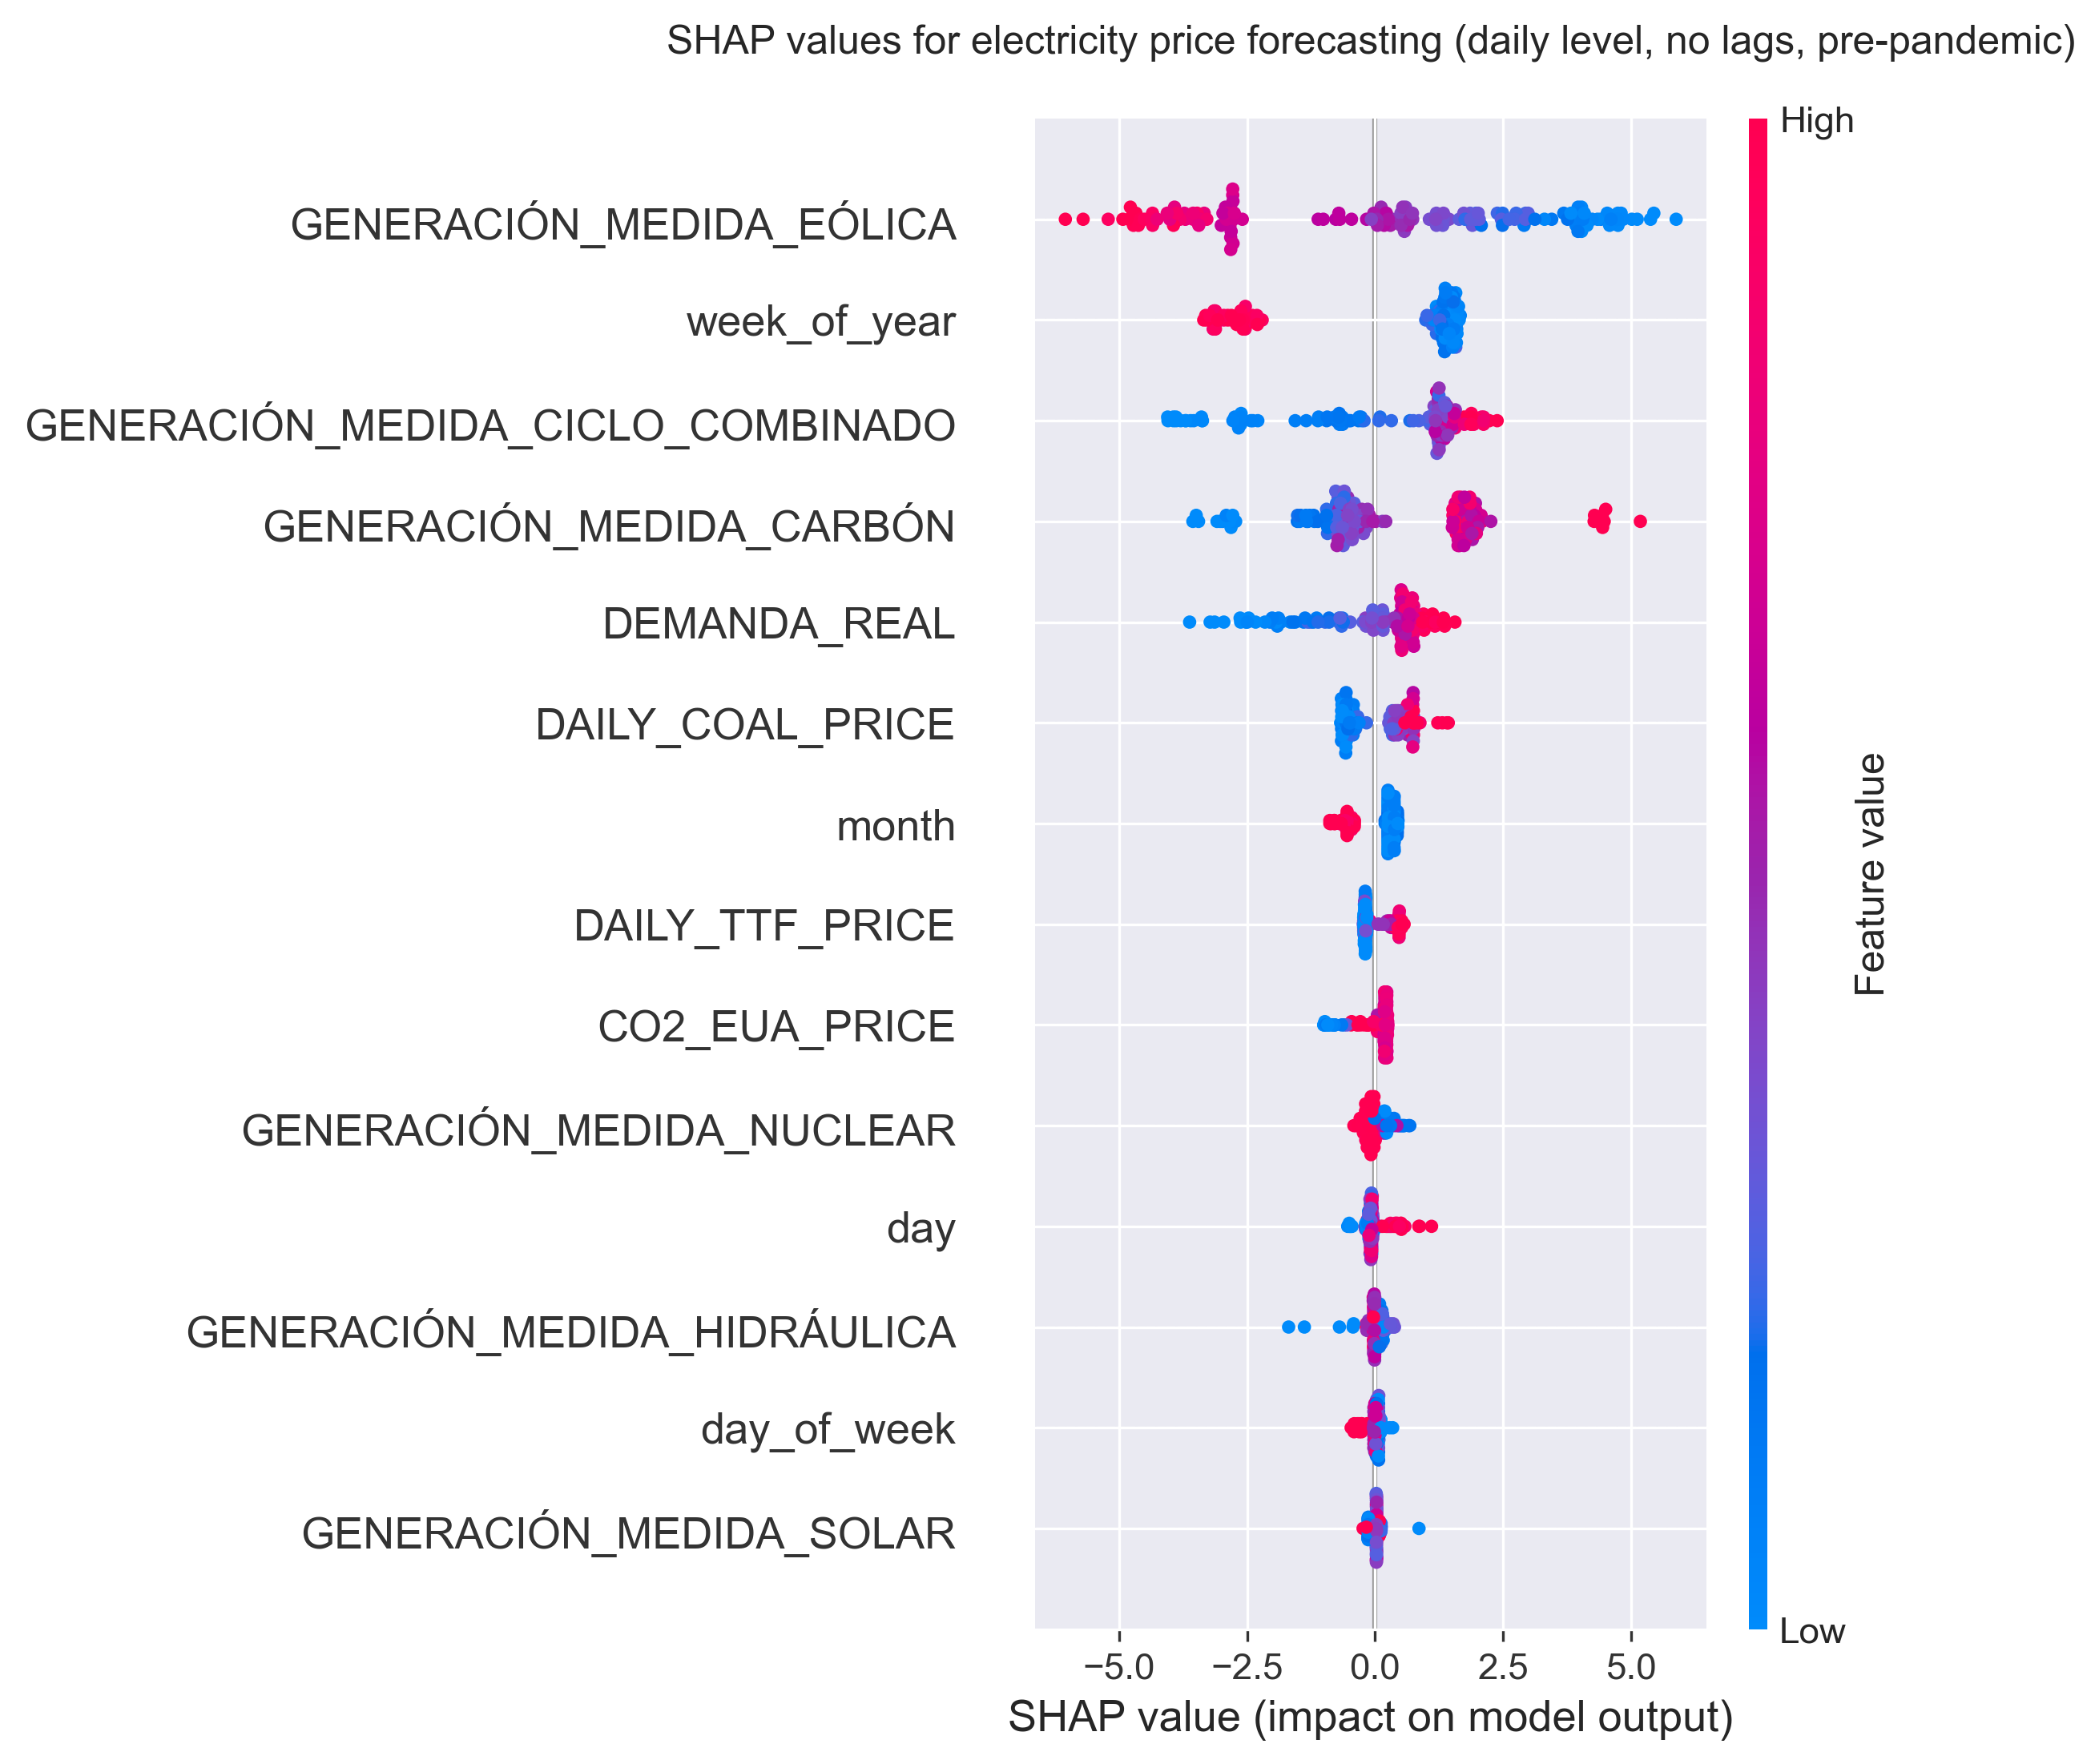
\includegraphics[width=1\linewidth]{images/analysis/shap-daily-pre-nolags}
        \caption{fh=30}
    \end{subfigure}

    \caption{SHAP values for the daily pre-pandemic energy price forecasting.}
    \label{fig:shap-daily-pre}
\end{figure}

We see how wind power, coal and combined cycle generation are the predictors influencing the forecast the most. As can be checked, high levels of wind power generation tend to lower the electricity price, while high level of combined cycle or coal generation tend to increase it. Between the date predictors, the one which stands out the most is the week of the year. Finally, the most important lag is 1, something that makes sense as is the closest to the response.

\subsection{After-Unkraine war scenario}
Let's now explore the after-war scenario. Data in use ranges from 2021-04-01 to 2023-03-31, and the best performing model changes to RF as seen in Table \ref{tab:cv-daily-post}.

\begin{table}[H]
\centering
\begin{tabular}{@{}l|l|l@{}}
\toprule
Model & MASE  & Modelling time (s)  \\ \midrule
RF    & 1.936 & 104.51  \\
GBT   & 2.153 & 67.30   \\
kNN   & 2.334 & 140.16  \\ \bottomrule
\end{tabular}
\caption{Model performance comparison trained over the daily post-war energy price.}
\label{tab:cv-daily-post}
\end{table}

After training RF with the complete cross-validation data and assessing the performance over the test partition, the MASE obtained is of 1.585. The result is shown in Figure \ref{fig:forecast-daily-post}.

\begin{figure}[H]
\centering
    \caption{Final forecasting of daily post-war energy price.}
    \label{fig:forecast-daily-post}
    \fbox{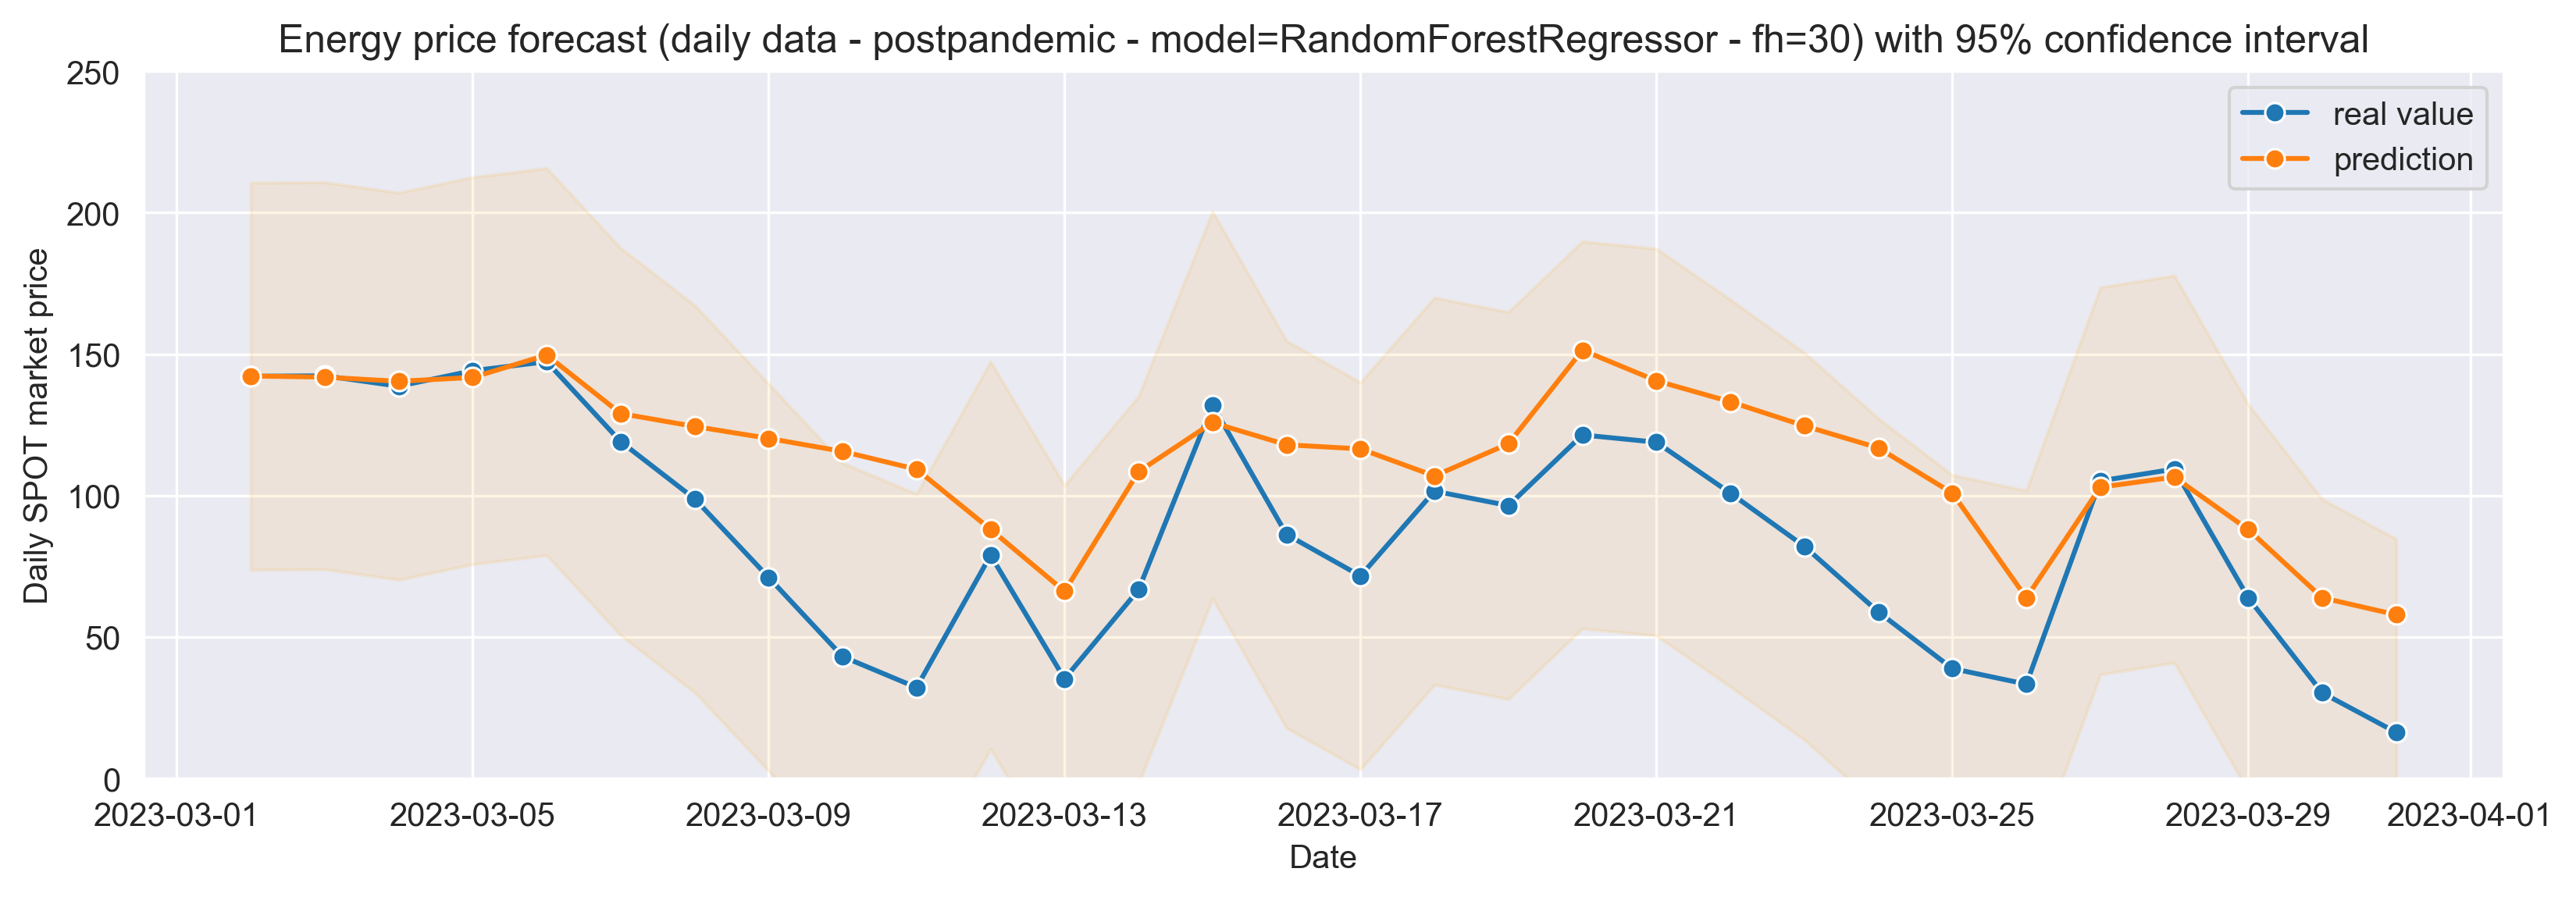
\includegraphics[scale=0.4]{images/analysis/forecast-daily-post}}
\end{figure}

Finally, let's compute the SHAP values.
%Looking at SHAP values we see similar tendencies to what seen in the pre-pandemic situation. Clean energies tend to reduce price while commodity-based generation technologies increase it. Nevertheless, the impact on the model output in the post-war situation is generally higher because the SHAP values show also larger values.
%
\begin{figure}[H]
\centering
    \begin{subfigure}{.45\textwidth}
        \centering
        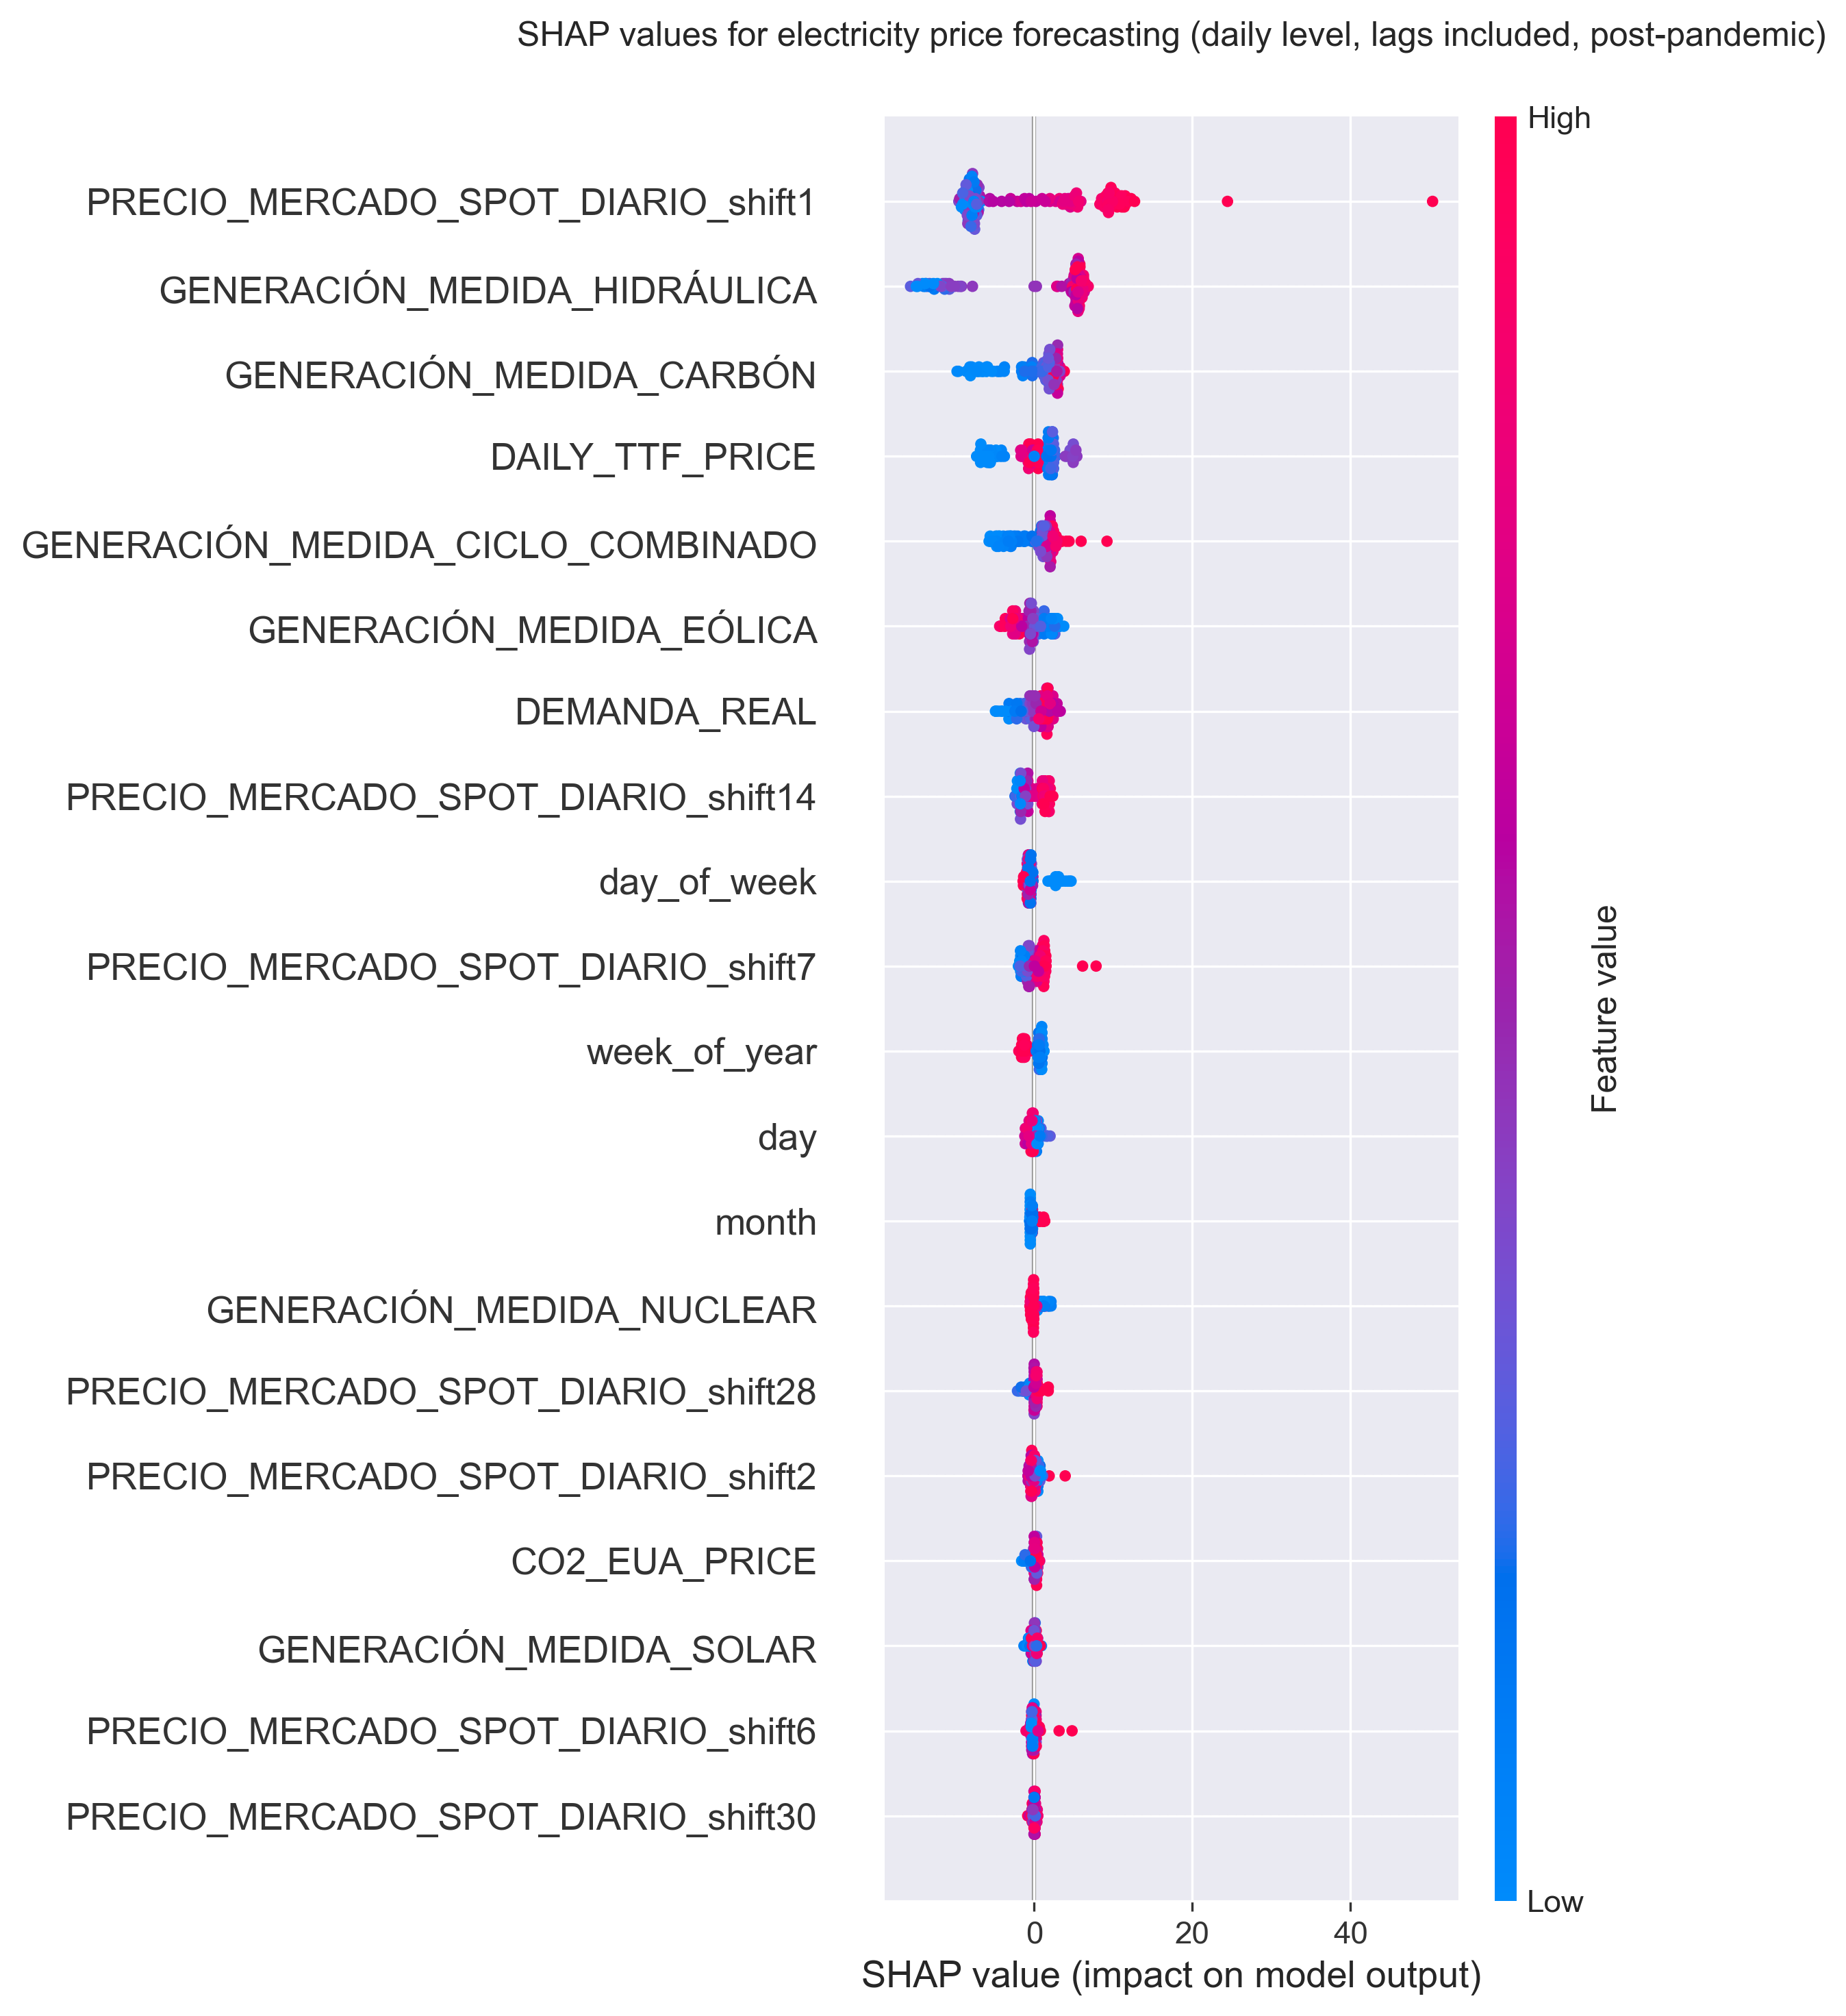
\includegraphics[width=1\linewidth]{images/analysis/shap-daily-post}
        \caption{fh=1}
    \end{subfigure}
    \begin{subfigure}{.45\textwidth}
        \centering
        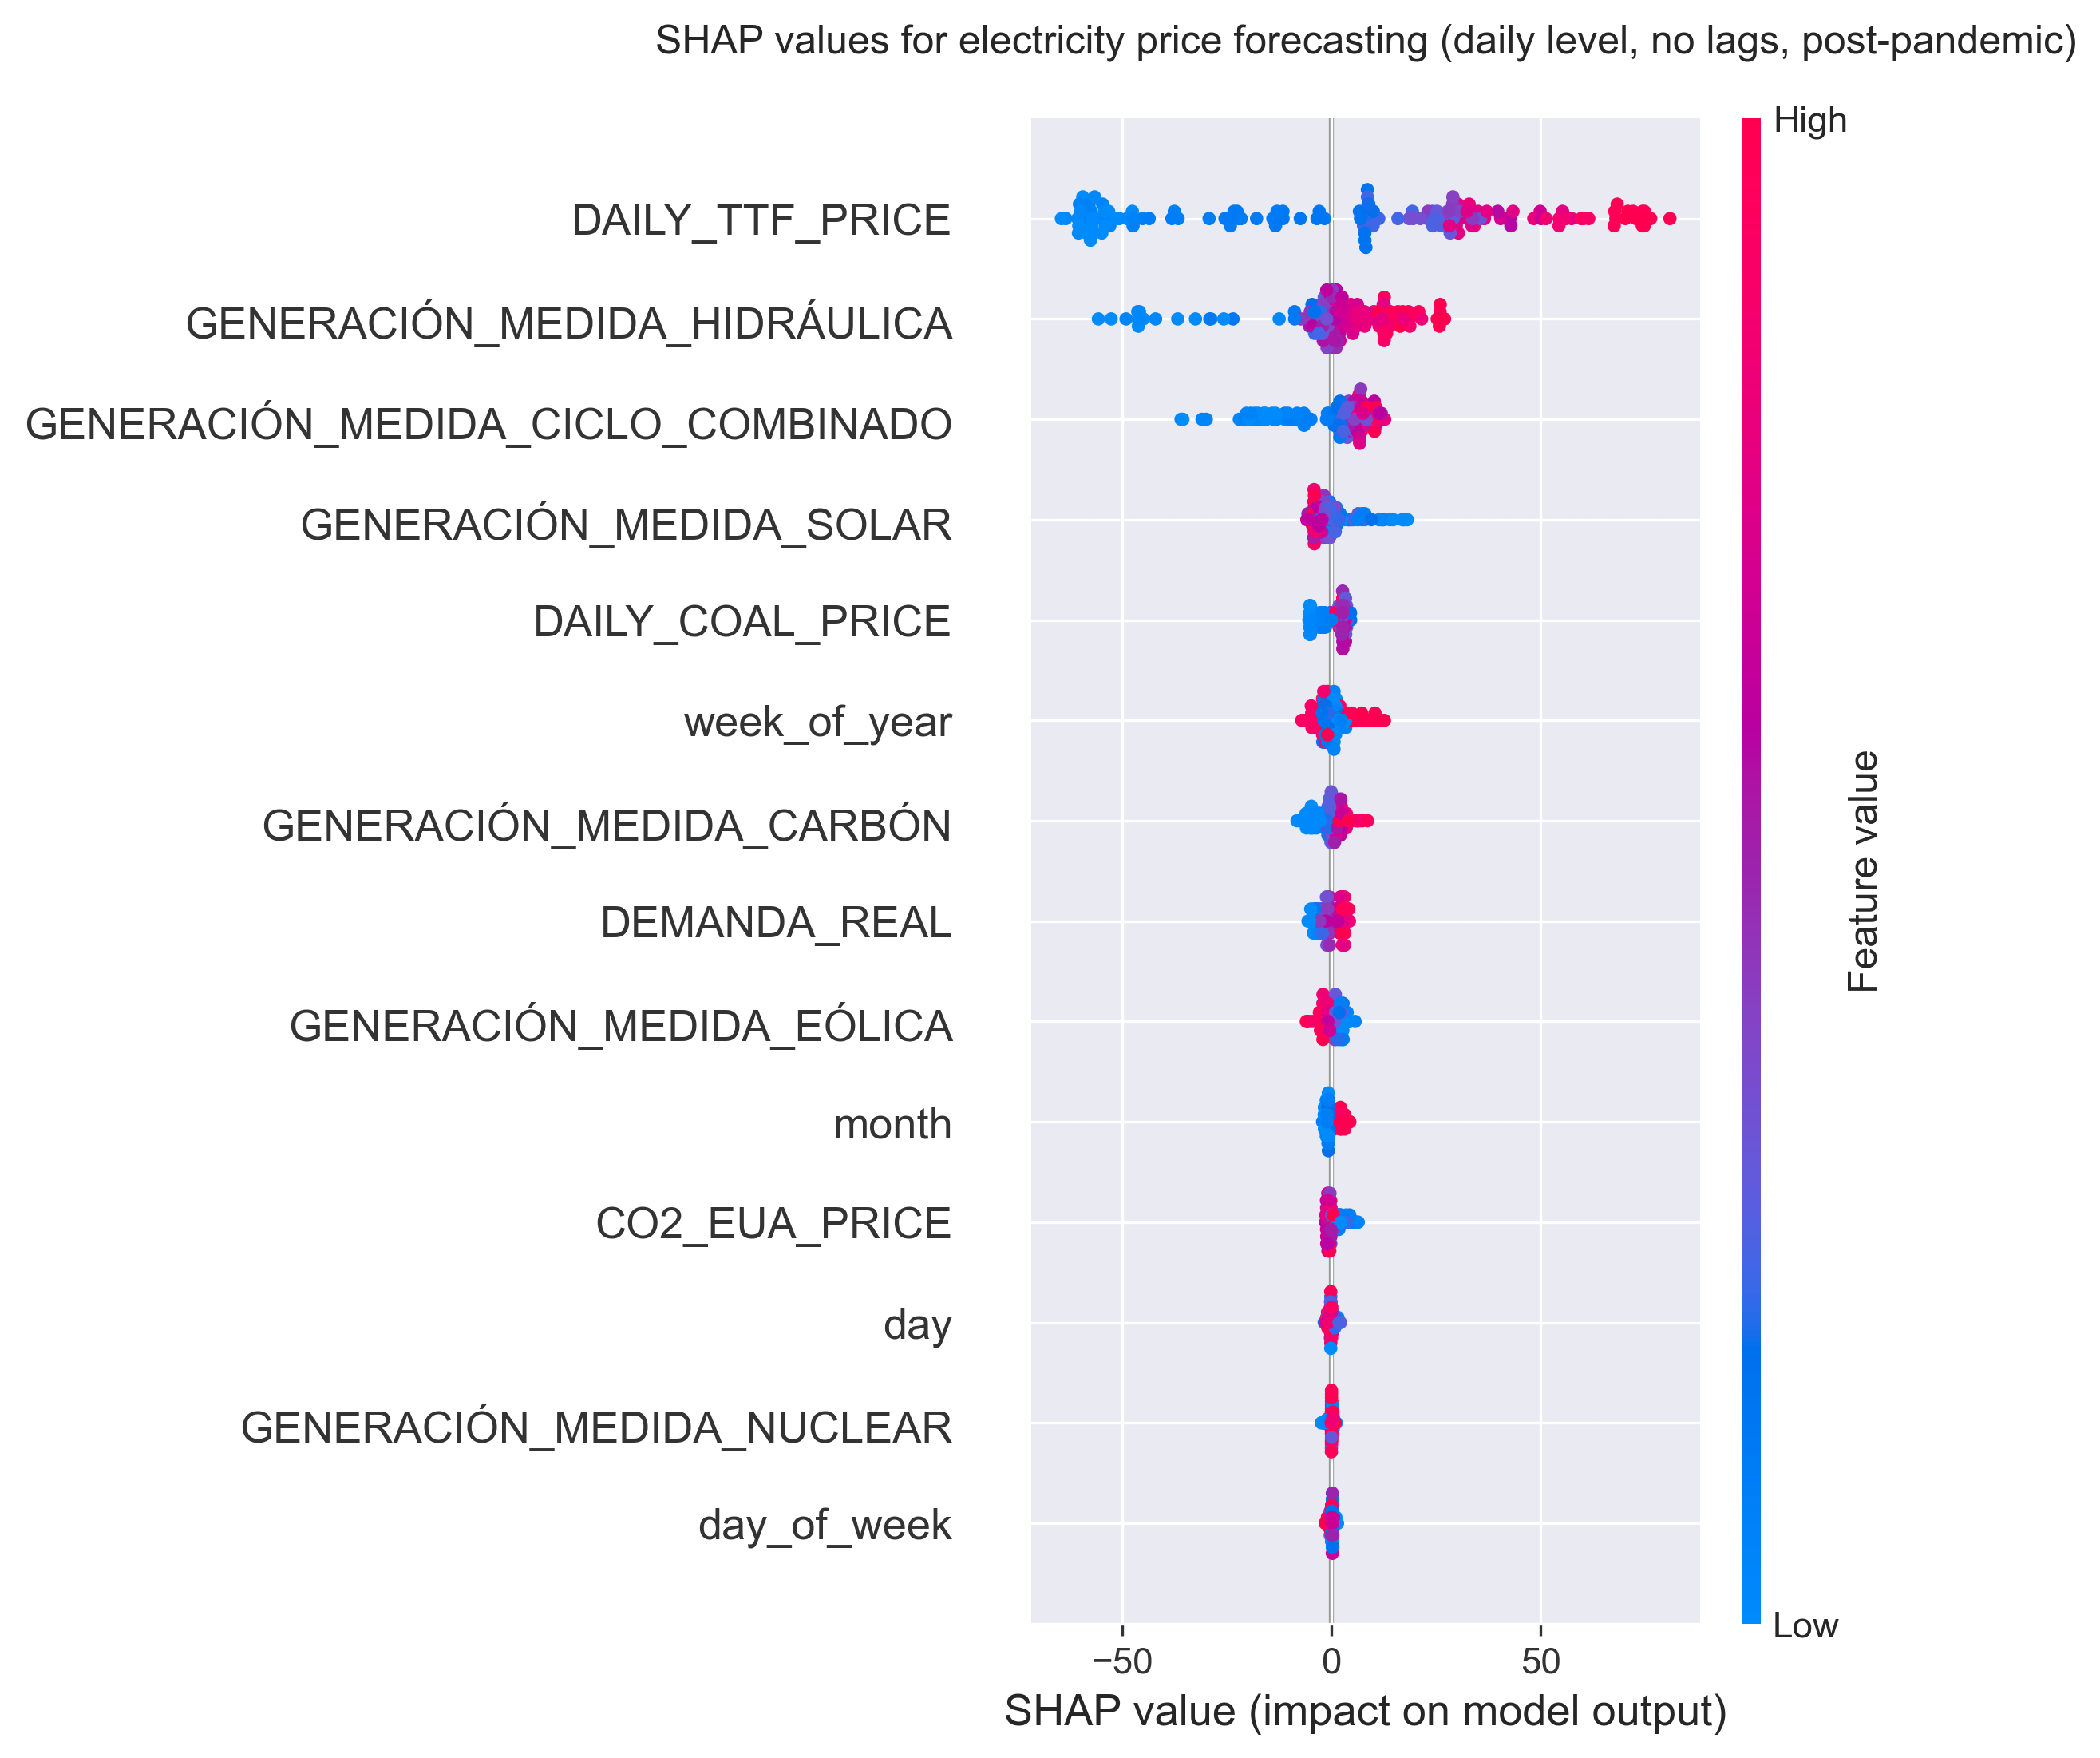
\includegraphics[width=1\linewidth]{images/analysis/shap-daily-post-nolags}
        \caption{fh=30}
    \end{subfigure}

    \caption{SHAP values for the daily post-war energy price forecasting.}
    \label{fig:shap-daily-post}
\end{figure}

Again, lag 1 is the most influencing lag. Before, the renewable technology most influencing the price was wind power, but now it changes to hydropower. Coal and combined cycle are

\subsection{Result discussion}



\section{Monthly analysis}
In the monthly level the author won't compare pre-pandemic with post-war markets as there are no enough datapoints. He will perform the study over the complete series, with data from 2014-01 to 2023-03.

The same predictors as before are used, except those related with date, which change:
\begin{itemize}
    \item \textbf{Date predictors:} Month and year.
\end{itemize}

%The best model now is the one based on Support Vector Machine

\begin{table}[H]
\centering
\begin{tabular}{@{}l|l|l@{}}
\toprule
Model & MASE  & Modelling time (s)  \\ \midrule
GBT   & 1.690  & 84.55    \\
RF    & 1.749  & 117.03   \\
kNN   & 2.662  & 108.33   \\ \bottomrule
\end{tabular}
\caption{}
\label{tab:cv-daily}
\end{table}

\begin{figure}[H]
\centering
    \caption{Final forecasting of monthly energy price.}
    \label{fig:forecast-monthly}
    \fbox{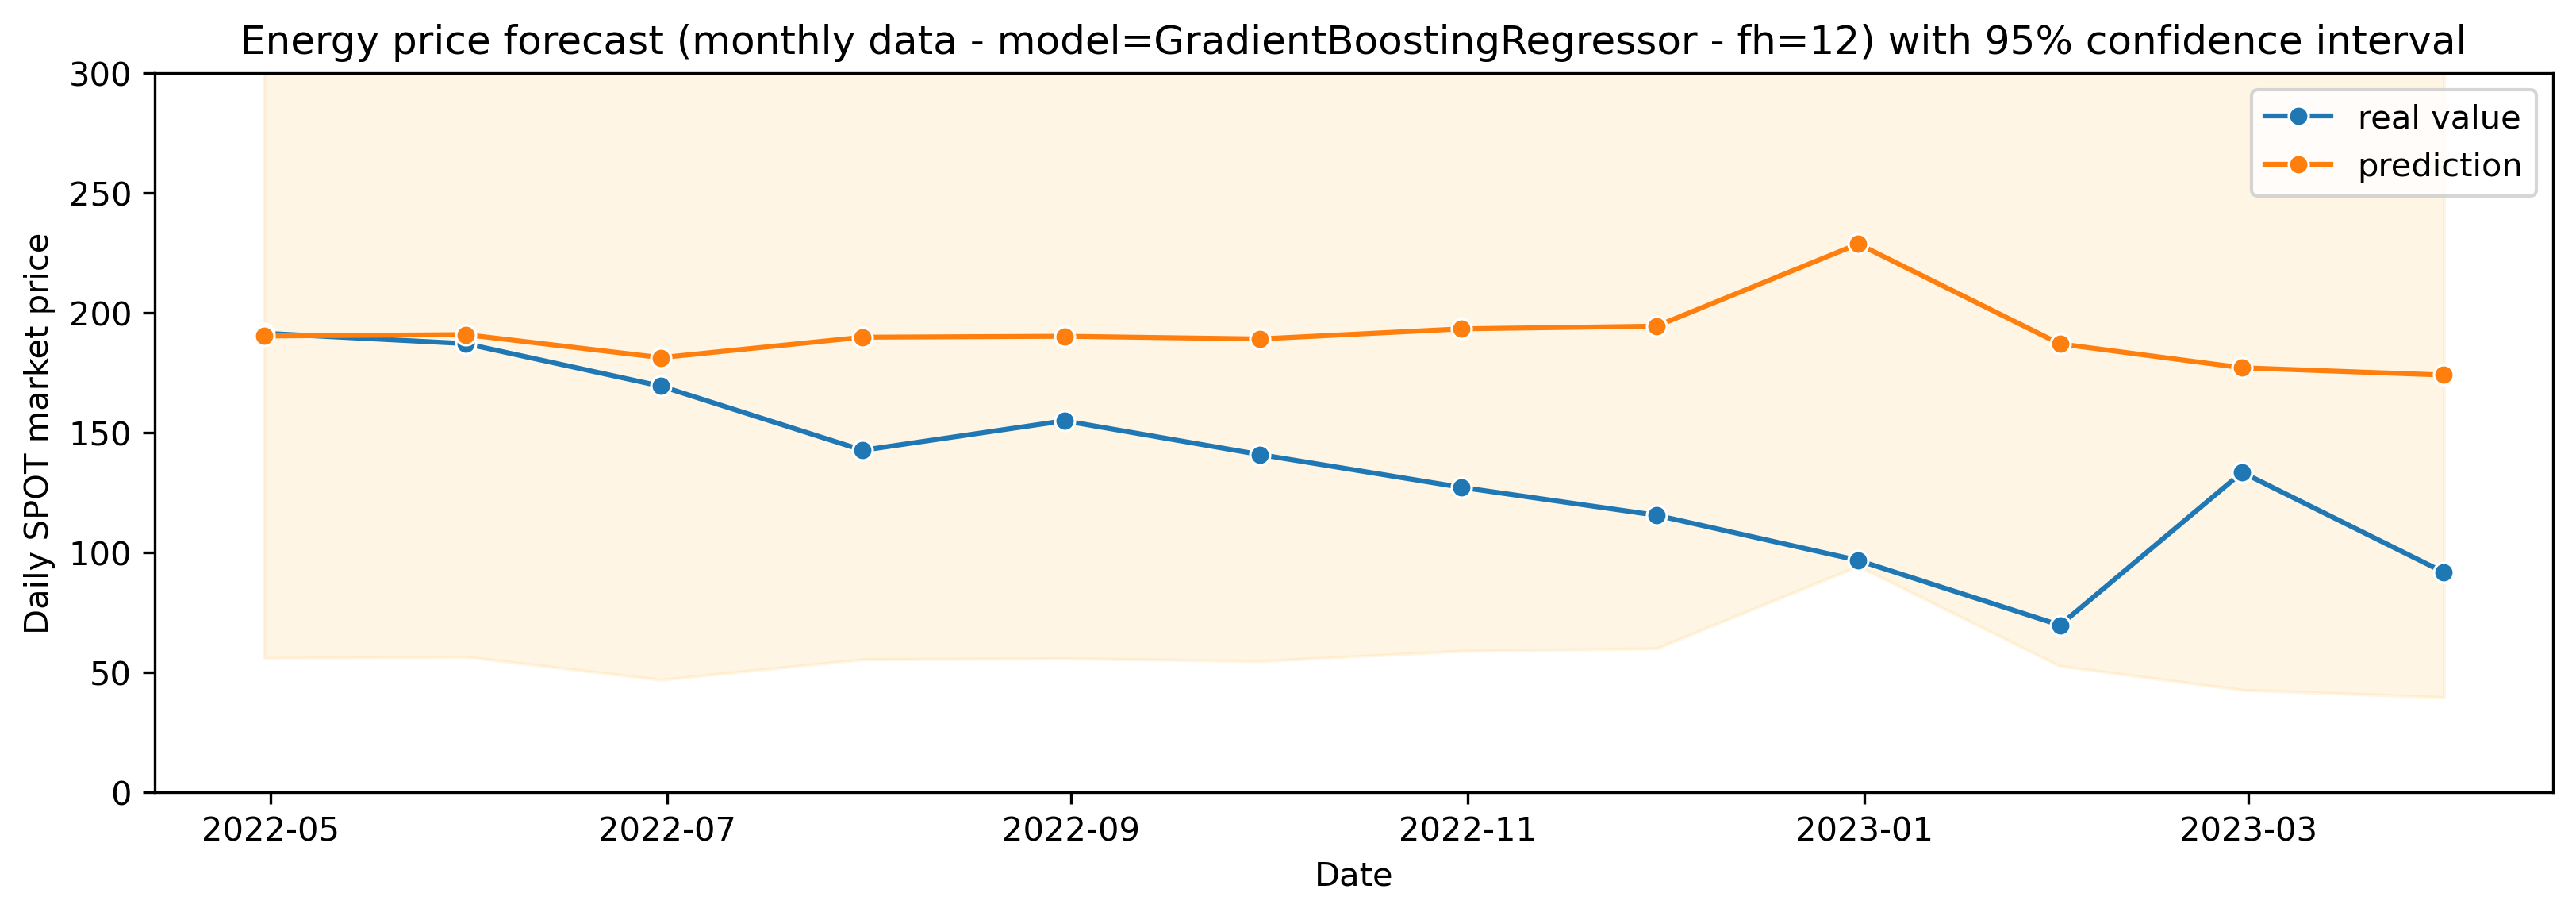
\includegraphics[scale=0.4]{images/analysis/forecast-monthly}}
\end{figure}

\begin{figure}[H]
\centering
    \begin{subfigure}{.45\textwidth}
        \centering
        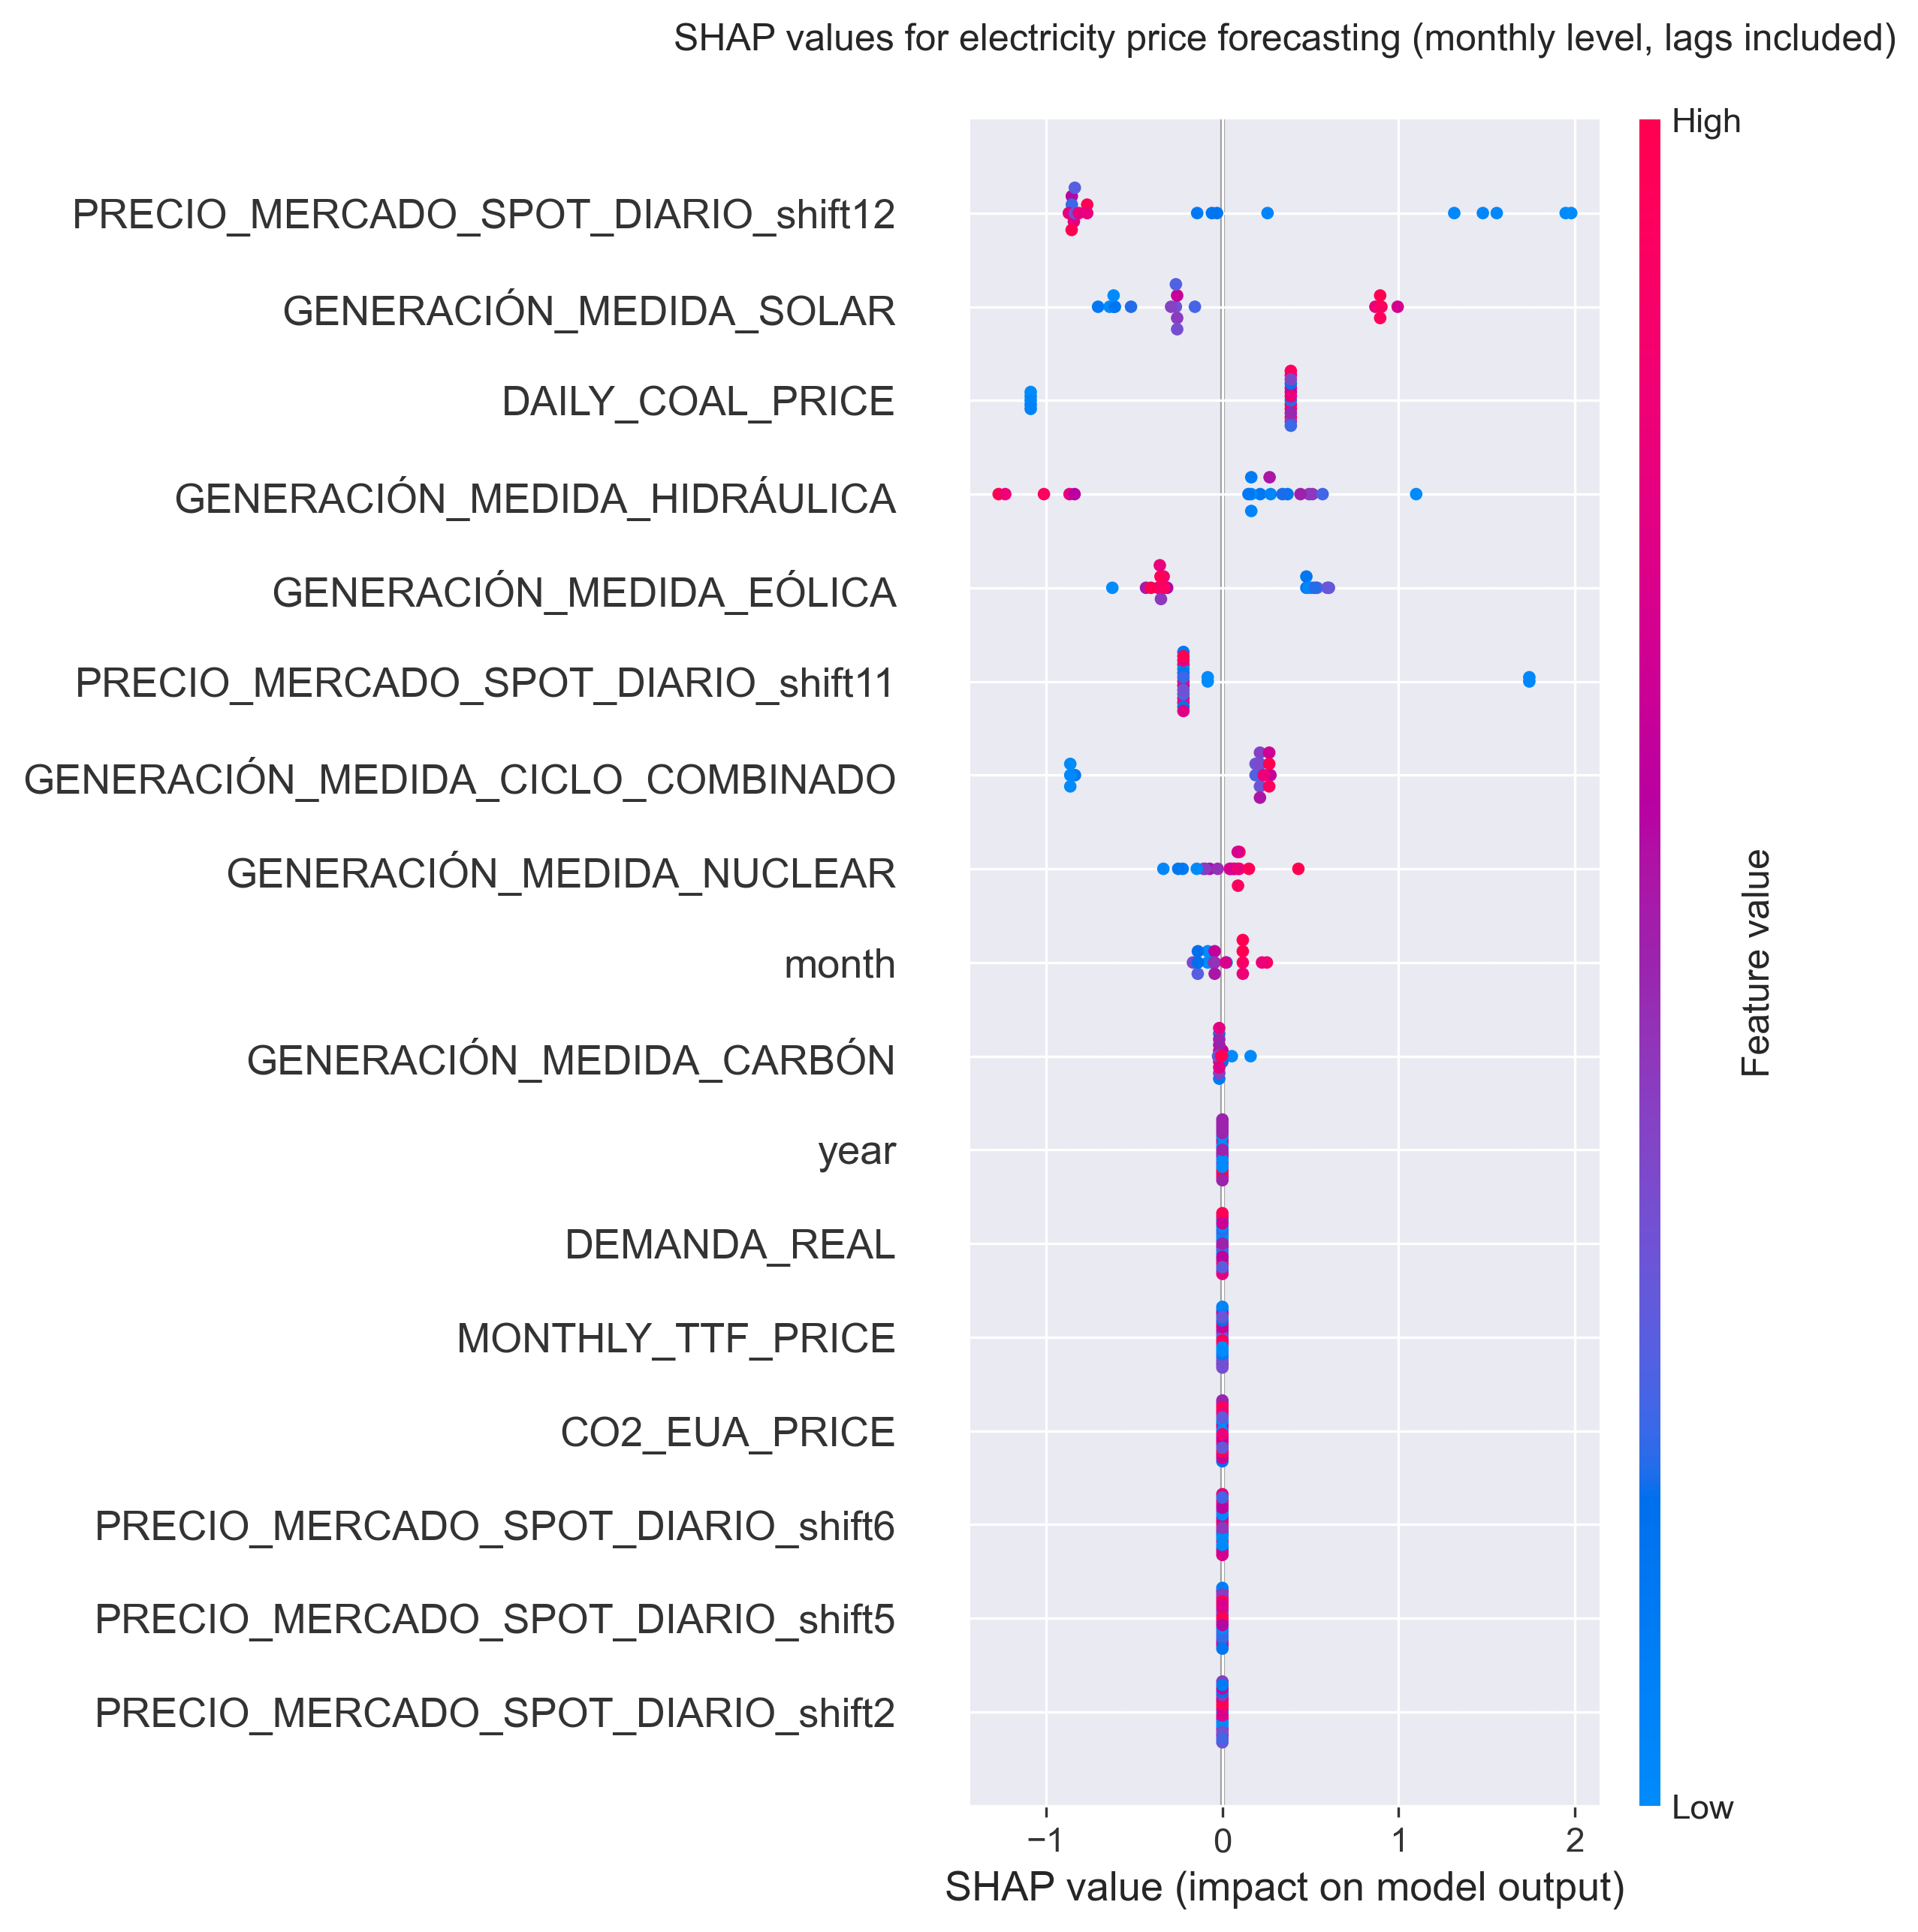
\includegraphics[width=1\linewidth]{images/analysis/shap-monthly}
        \caption{fh=1}
    \end{subfigure}
    \begin{subfigure}{.45\textwidth}
        \centering
        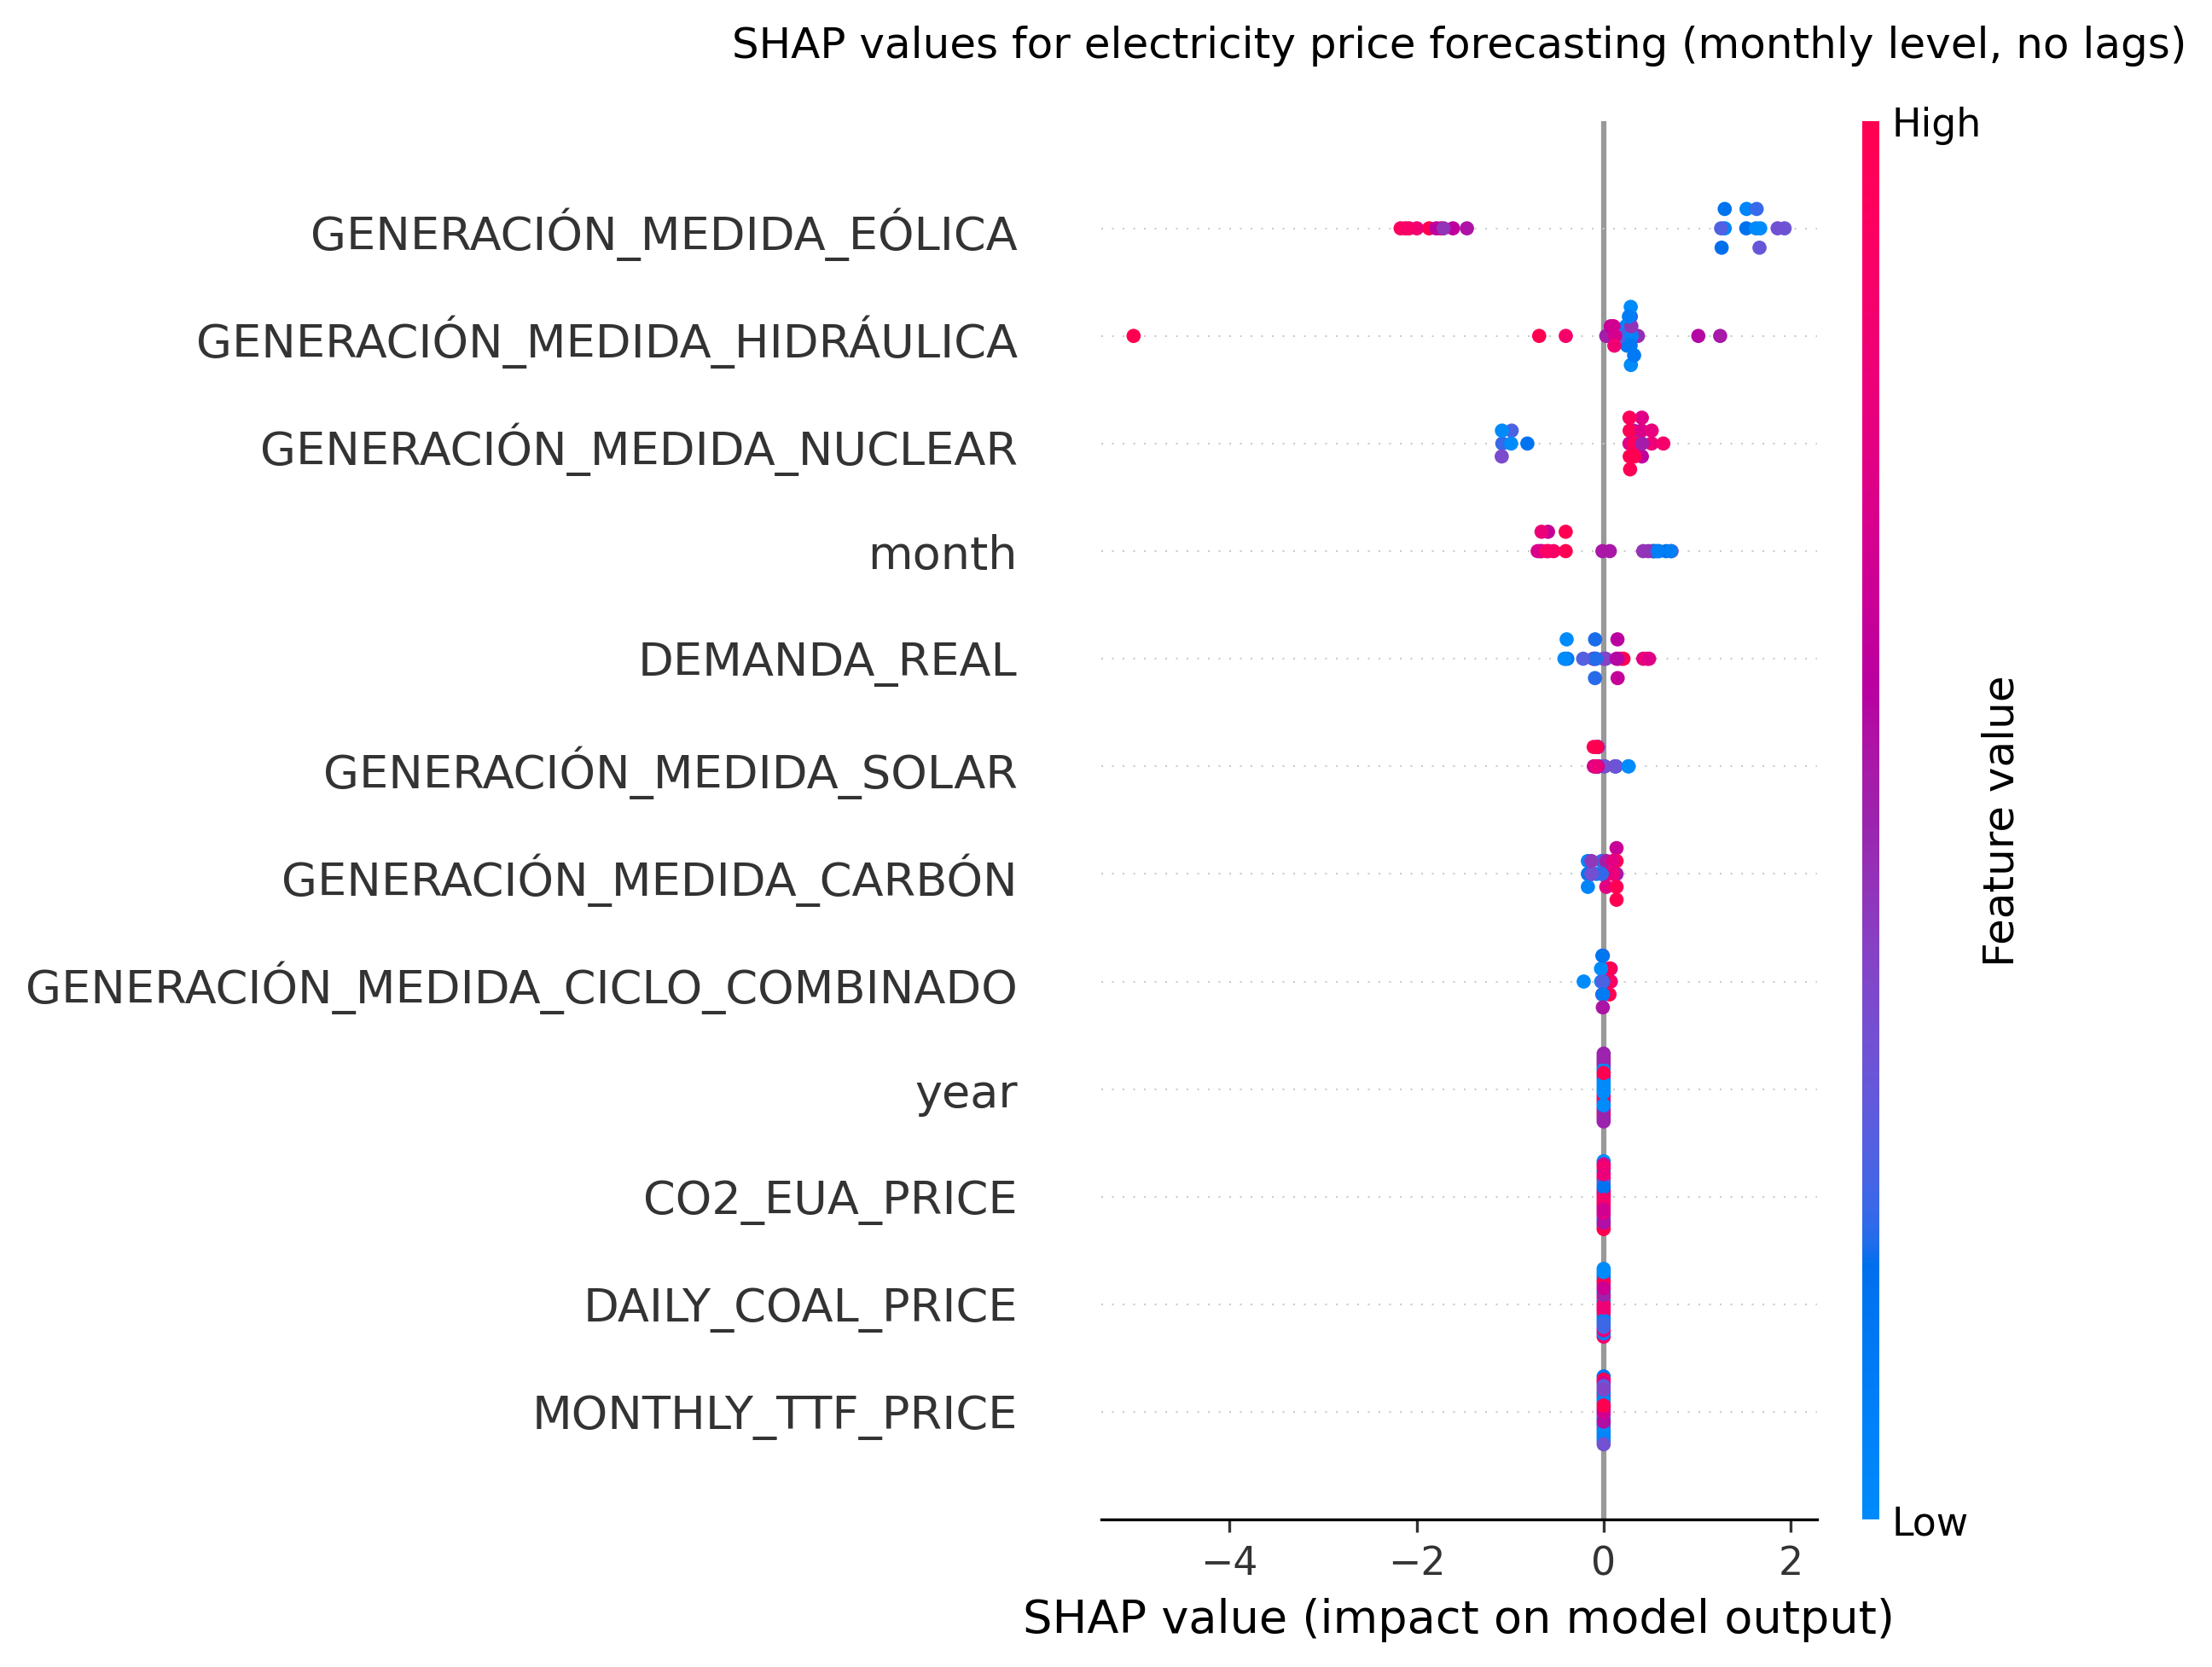
\includegraphics[width=1\linewidth]{images/analysis/shap-monthly-nolags}
        \caption{fh=12}
    \end{subfigure}

    \caption{SHAP values for the monthly energy price forecasting.}
    \label{fig:shap-monthly}
\end{figure}



\section{Yearly analysis}
\chapter{Conclusions}
In this Master Thesis, the author has forecasted electricity prices and analyzed which variables are influencing the prediction. This analysis has been done in an hourly, daily (short term), monthly (medium term) and yearly  (long term) fashion, as each aggregation has different properties. This project has not only helped the author to begin to understand the electricity market, but to learn how to work with time series.

About the results obtained in the forecasts it can be seen how tree based algorithms performed the best, compared with distance based ones. Apart, modeling the short term has been easier than forecasting the medium, probably due to the higher number of datapoints in the former or the patterns in the series that make it more modelable. The MASEs obtained in the medium term are higher and the prediction intervals are broader, compared with those in the short term forecasts.

The results show that the probably most important predictor in the short term forecast is combined cycle generation: when predicting in an hourly fashion, it's the one that always appears in the top, together with some lags. In the daily aggregation this predictor still appears, but others related with renewable technologies such as wind power or hydropower also are important, apart from coal generation. The use of wind power seems to reduce electricity price, while the others contribute to increase it. In the monthly aggregation, results are not conclusive, probably due to the lack of datapoints.

About pre-covid and post-war markets, in hourly and daily aggregations, the MASE obtained in post-war is always higher. This is probably due to the higher uncertainty on this period. About predictor importance, the tendencies in both periods are similar.

The yearly analysis has been done not analytically but in a descriptive way, due to the lack of data. On it, commodity prices seem to be the main driver of electricity price. The increase in solar and wind power generation could help to reduce their influence in the following years.

Finally, by conducting this Thesis, the author has discovered the state of the art in time series. He has learned how to work with the main libraries in Python, downloading and managing data retrieved from an API.

%----------
%	BIBLIOGRAFÍA
%----------	

%\nocite{*} % Si quieres que aparezcan en la bibliografía todos los documentos que la componen (también los que no estén citados en el texto) descomenta está lína

\clearpage
\addcontentsline{toc}{chapter}{Bibliography}
\printbibliography



%----------
%	ANEXOS
%----------	

% Si tu trabajo incluye anexos, puedes descomentar las siguientes líneas
%\chapter* {Annexes x}
%\pagenumbering{gobble} % Las páginas de los anexos no se numeran



\end{document}